% Minimal sebenta template generated automatically
\documentclass[11pt,a4paper]{article}
\usepackage[utf8]{inputenc}
\usepackage[T1]{fontenc}
\usepackage{lmodern}
\usepackage{geometry}
\usepackage{fancyhdr}
\usepackage{hyperref}
\usepackage{graphicx}
\usepackage{float}
\usepackage{placeins}
\usepackage{bookmark}
\usepackage{booktabs}
\usepackage{amsmath,amssymb}
\usepackage{csquotes}
\usepackage{enumitem}
\usepackage{tikz}
\IfFileExists{pgfplots.sty}{\usepackage{pgfplots}\pgfplotsset{compat=1.17}}{}

\geometry{margin=2.5cm}

% Try to include project-specific style macros (containing \exercicio, \subexercicio, etc.)
% Try multiple relative locations to be robust across different generated output paths
\IfFileExists{../../../../Teste_modelo/config/style.tex}{% Sistema de exercícios com contadores automáticos
\newcounter{exerciciocount}          % Contador principal dos exercícios
\newcounter{subexerciciocount}       % Contador dos subexercícios
\newcounter{optioncount}             % Contador das opções

% Control whether the macro prints the automatic "Exercício N." heading.
% Default: show the heading. Call \showexerciciotitlefalse to suppress.
\newif\ifshowexerciciotitle
\showexerciciotitletrue

% Macro para exercício principal
\newcommand{\exercicio}[1]{%
        \par\vspace{1.5em}% Espaçamento antes
        \refstepcounter{exerciciocount}% Incrementa contador principal
        \setcounter{subexerciciocount}{0}% Reseta contador de subexercícios
        \setcounter{optioncount}{0}% Reseta contador de opções
        % Only print the automatic heading if the flag is true
        \ifshowexerciciotitle
            \noindent\textbf{Exercício~\theexerciciocount.}\space #1\par\vspace{0.5em}%
        \else
            % When suppressed, just print the content without the heading
            #1\par\vspace{0.5em}%
        \fi
}

% Macro para subexercício
\newcommand{\subexercicio}[1]{%
    \par\vspace{0.8em}% Espaçamento menor para subexercícios
    \refstepcounter{subexerciciocount}% Incrementa contador de subexercícios
    \noindent\textbf{\theexerciciocount.\thesubexerciciocount.} #1\par\vspace{0.3em}%
}

% Macro para opção
\newcommand{\option}[1]{%
    \par
    \refstepcounter{optioncount}%
    \noindent(\alph{optioncount}) #1%
}

% Título e informações do exame
\title{1ª Questão de aula do Módulo A10: Otimização}
\author{EPRALIMA - Escola Profissional Alto Lima}

\date{}

% Cabeçalho completo do teste dentro de uma caixa simples
\newcommand{\espacoAluno}{%
    \vspace{0.5cm}
    \fbox{%
        \parbox{\textwidth}{%
            \noindent\textbf{Nome do Aluno:} \underline{\hspace{7cm}} \textbf{Turma:} \underline{\hspace{1cm}}\\[0.5cm]
            \noindent\textbf{Assinatura do Professor:} \underline{\hspace{3cm}} \hfill \textbf{Nota:} \underline{\hspace{2cm}}\\[0.5cm]
            \noindent\textbf{Assinatura do Encarregado de Educação:} \underline{\hspace{3cm}}
        }%
    }
    \vspace{1cm}
}}{%
  \IfFileExists{../../../Teste_modelo/config/style.tex}{% Sistema de exercícios com contadores automáticos
\newcounter{exerciciocount}          % Contador principal dos exercícios
\newcounter{subexerciciocount}       % Contador dos subexercícios
\newcounter{optioncount}             % Contador das opções

% Control whether the macro prints the automatic "Exercício N." heading.
% Default: show the heading. Call \showexerciciotitlefalse to suppress.
\newif\ifshowexerciciotitle
\showexerciciotitletrue

% Macro para exercício principal
\newcommand{\exercicio}[1]{%
        \par\vspace{1.5em}% Espaçamento antes
        \refstepcounter{exerciciocount}% Incrementa contador principal
        \setcounter{subexerciciocount}{0}% Reseta contador de subexercícios
        \setcounter{optioncount}{0}% Reseta contador de opções
        % Only print the automatic heading if the flag is true
        \ifshowexerciciotitle
            \noindent\textbf{Exercício~\theexerciciocount.}\space #1\par\vspace{0.5em}%
        \else
            % When suppressed, just print the content without the heading
            #1\par\vspace{0.5em}%
        \fi
}

% Macro para subexercício
\newcommand{\subexercicio}[1]{%
    \par\vspace{0.8em}% Espaçamento menor para subexercícios
    \refstepcounter{subexerciciocount}% Incrementa contador de subexercícios
    \noindent\textbf{\theexerciciocount.\thesubexerciciocount.} #1\par\vspace{0.3em}%
}

% Macro para opção
\newcommand{\option}[1]{%
    \par
    \refstepcounter{optioncount}%
    \noindent(\alph{optioncount}) #1%
}

% Título e informações do exame
\title{1ª Questão de aula do Módulo A10: Otimização}
\author{EPRALIMA - Escola Profissional Alto Lima}

\date{}

% Cabeçalho completo do teste dentro de uma caixa simples
\newcommand{\espacoAluno}{%
    \vspace{0.5cm}
    \fbox{%
        \parbox{\textwidth}{%
            \noindent\textbf{Nome do Aluno:} \underline{\hspace{7cm}} \textbf{Turma:} \underline{\hspace{1cm}}\\[0.5cm]
            \noindent\textbf{Assinatura do Professor:} \underline{\hspace{3cm}} \hfill \textbf{Nota:} \underline{\hspace{2cm}}\\[0.5cm]
            \noindent\textbf{Assinatura do Encarregado de Educação:} \underline{\hspace{3cm}}
        }%
    }
    \vspace{1cm}
}}{%
    \IfFileExists{../../Teste_modelo/config/style.tex}{% Sistema de exercícios com contadores automáticos
\newcounter{exerciciocount}          % Contador principal dos exercícios
\newcounter{subexerciciocount}       % Contador dos subexercícios
\newcounter{optioncount}             % Contador das opções

% Control whether the macro prints the automatic "Exercício N." heading.
% Default: show the heading. Call \showexerciciotitlefalse to suppress.
\newif\ifshowexerciciotitle
\showexerciciotitletrue

% Macro para exercício principal
\newcommand{\exercicio}[1]{%
        \par\vspace{1.5em}% Espaçamento antes
        \refstepcounter{exerciciocount}% Incrementa contador principal
        \setcounter{subexerciciocount}{0}% Reseta contador de subexercícios
        \setcounter{optioncount}{0}% Reseta contador de opções
        % Only print the automatic heading if the flag is true
        \ifshowexerciciotitle
            \noindent\textbf{Exercício~\theexerciciocount.}\space #1\par\vspace{0.5em}%
        \else
            % When suppressed, just print the content without the heading
            #1\par\vspace{0.5em}%
        \fi
}

% Macro para subexercício
\newcommand{\subexercicio}[1]{%
    \par\vspace{0.8em}% Espaçamento menor para subexercícios
    \refstepcounter{subexerciciocount}% Incrementa contador de subexercícios
    \noindent\textbf{\theexerciciocount.\thesubexerciciocount.} #1\par\vspace{0.3em}%
}

% Macro para opção
\newcommand{\option}[1]{%
    \par
    \refstepcounter{optioncount}%
    \noindent(\alph{optioncount}) #1%
}

% Título e informações do exame
\title{1ª Questão de aula do Módulo A10: Otimização}
\author{EPRALIMA - Escola Profissional Alto Lima}

\date{}

% Cabeçalho completo do teste dentro de uma caixa simples
\newcommand{\espacoAluno}{%
    \vspace{0.5cm}
    \fbox{%
        \parbox{\textwidth}{%
            \noindent\textbf{Nome do Aluno:} \underline{\hspace{7cm}} \textbf{Turma:} \underline{\hspace{1cm}}\\[0.5cm]
            \noindent\textbf{Assinatura do Professor:} \underline{\hspace{3cm}} \hfill \textbf{Nota:} \underline{\hspace{2cm}}\\[0.5cm]
            \noindent\textbf{Assinatura do Encarregado de Educação:} \underline{\hspace{3cm}}
        }%
    }
    \vspace{1cm}
}}{%
      % style.tex not found - proceed without project macros
    }%
  }%
}

% Provide a robust fallback for macros that might be missing in style.tex
% This attempts to include the project style first (multiple relative paths),
% and only if none exist defines minimal counters and macros safely.
\IfFileExists{../../../../Teste_modelo/config/style.tex}{% Sistema de exercícios com contadores automáticos
\newcounter{exerciciocount}          % Contador principal dos exercícios
\newcounter{subexerciciocount}       % Contador dos subexercícios
\newcounter{optioncount}             % Contador das opções

% Control whether the macro prints the automatic "Exercício N." heading.
% Default: show the heading. Call \showexerciciotitlefalse to suppress.
\newif\ifshowexerciciotitle
\showexerciciotitletrue

% Macro para exercício principal
\newcommand{\exercicio}[1]{%
        \par\vspace{1.5em}% Espaçamento antes
        \refstepcounter{exerciciocount}% Incrementa contador principal
        \setcounter{subexerciciocount}{0}% Reseta contador de subexercícios
        \setcounter{optioncount}{0}% Reseta contador de opções
        % Only print the automatic heading if the flag is true
        \ifshowexerciciotitle
            \noindent\textbf{Exercício~\theexerciciocount.}\space #1\par\vspace{0.5em}%
        \else
            % When suppressed, just print the content without the heading
            #1\par\vspace{0.5em}%
        \fi
}

% Macro para subexercício
\newcommand{\subexercicio}[1]{%
    \par\vspace{0.8em}% Espaçamento menor para subexercícios
    \refstepcounter{subexerciciocount}% Incrementa contador de subexercícios
    \noindent\textbf{\theexerciciocount.\thesubexerciciocount.} #1\par\vspace{0.3em}%
}

% Macro para opção
\newcommand{\option}[1]{%
    \par
    \refstepcounter{optioncount}%
    \noindent(\alph{optioncount}) #1%
}

% Título e informações do exame
\title{1ª Questão de aula do Módulo A10: Otimização}
\author{EPRALIMA - Escola Profissional Alto Lima}

\date{}

% Cabeçalho completo do teste dentro de uma caixa simples
\newcommand{\espacoAluno}{%
    \vspace{0.5cm}
    \fbox{%
        \parbox{\textwidth}{%
            \noindent\textbf{Nome do Aluno:} \underline{\hspace{7cm}} \textbf{Turma:} \underline{\hspace{1cm}}\\[0.5cm]
            \noindent\textbf{Assinatura do Professor:} \underline{\hspace{3cm}} \hfill \textbf{Nota:} \underline{\hspace{2cm}}\\[0.5cm]
            \noindent\textbf{Assinatura do Encarregado de Educação:} \underline{\hspace{3cm}}
        }%
    }
    \vspace{1cm}
}}{%
  \IfFileExists{../../../Teste_modelo/config/style.tex}{% Sistema de exercícios com contadores automáticos
\newcounter{exerciciocount}          % Contador principal dos exercícios
\newcounter{subexerciciocount}       % Contador dos subexercícios
\newcounter{optioncount}             % Contador das opções

% Control whether the macro prints the automatic "Exercício N." heading.
% Default: show the heading. Call \showexerciciotitlefalse to suppress.
\newif\ifshowexerciciotitle
\showexerciciotitletrue

% Macro para exercício principal
\newcommand{\exercicio}[1]{%
        \par\vspace{1.5em}% Espaçamento antes
        \refstepcounter{exerciciocount}% Incrementa contador principal
        \setcounter{subexerciciocount}{0}% Reseta contador de subexercícios
        \setcounter{optioncount}{0}% Reseta contador de opções
        % Only print the automatic heading if the flag is true
        \ifshowexerciciotitle
            \noindent\textbf{Exercício~\theexerciciocount.}\space #1\par\vspace{0.5em}%
        \else
            % When suppressed, just print the content without the heading
            #1\par\vspace{0.5em}%
        \fi
}

% Macro para subexercício
\newcommand{\subexercicio}[1]{%
    \par\vspace{0.8em}% Espaçamento menor para subexercícios
    \refstepcounter{subexerciciocount}% Incrementa contador de subexercícios
    \noindent\textbf{\theexerciciocount.\thesubexerciciocount.} #1\par\vspace{0.3em}%
}

% Macro para opção
\newcommand{\option}[1]{%
    \par
    \refstepcounter{optioncount}%
    \noindent(\alph{optioncount}) #1%
}

% Título e informações do exame
\title{1ª Questão de aula do Módulo A10: Otimização}
\author{EPRALIMA - Escola Profissional Alto Lima}

\date{}

% Cabeçalho completo do teste dentro de uma caixa simples
\newcommand{\espacoAluno}{%
    \vspace{0.5cm}
    \fbox{%
        \parbox{\textwidth}{%
            \noindent\textbf{Nome do Aluno:} \underline{\hspace{7cm}} \textbf{Turma:} \underline{\hspace{1cm}}\\[0.5cm]
            \noindent\textbf{Assinatura do Professor:} \underline{\hspace{3cm}} \hfill \textbf{Nota:} \underline{\hspace{2cm}}\\[0.5cm]
            \noindent\textbf{Assinatura do Encarregado de Educação:} \underline{\hspace{3cm}}
        }%
    }
    \vspace{1cm}
}}{%
    \IfFileExists{../../Teste_modelo/config/style.tex}{% Sistema de exercícios com contadores automáticos
\newcounter{exerciciocount}          % Contador principal dos exercícios
\newcounter{subexerciciocount}       % Contador dos subexercícios
\newcounter{optioncount}             % Contador das opções

% Control whether the macro prints the automatic "Exercício N." heading.
% Default: show the heading. Call \showexerciciotitlefalse to suppress.
\newif\ifshowexerciciotitle
\showexerciciotitletrue

% Macro para exercício principal
\newcommand{\exercicio}[1]{%
        \par\vspace{1.5em}% Espaçamento antes
        \refstepcounter{exerciciocount}% Incrementa contador principal
        \setcounter{subexerciciocount}{0}% Reseta contador de subexercícios
        \setcounter{optioncount}{0}% Reseta contador de opções
        % Only print the automatic heading if the flag is true
        \ifshowexerciciotitle
            \noindent\textbf{Exercício~\theexerciciocount.}\space #1\par\vspace{0.5em}%
        \else
            % When suppressed, just print the content without the heading
            #1\par\vspace{0.5em}%
        \fi
}

% Macro para subexercício
\newcommand{\subexercicio}[1]{%
    \par\vspace{0.8em}% Espaçamento menor para subexercícios
    \refstepcounter{subexerciciocount}% Incrementa contador de subexercícios
    \noindent\textbf{\theexerciciocount.\thesubexerciciocount.} #1\par\vspace{0.3em}%
}

% Macro para opção
\newcommand{\option}[1]{%
    \par
    \refstepcounter{optioncount}%
    \noindent(\alph{optioncount}) #1%
}

% Título e informações do exame
\title{1ª Questão de aula do Módulo A10: Otimização}
\author{EPRALIMA - Escola Profissional Alto Lima}

\date{}

% Cabeçalho completo do teste dentro de uma caixa simples
\newcommand{\espacoAluno}{%
    \vspace{0.5cm}
    \fbox{%
        \parbox{\textwidth}{%
            \noindent\textbf{Nome do Aluno:} \underline{\hspace{7cm}} \textbf{Turma:} \underline{\hspace{1cm}}\\[0.5cm]
            \noindent\textbf{Assinatura do Professor:} \underline{\hspace{3cm}} \hfill \textbf{Nota:} \underline{\hspace{2cm}}\\[0.5cm]
            \noindent\textbf{Assinatura do Encarregado de Educação:} \underline{\hspace{3cm}}
        }%
    }
    \vspace{1cm}
}}{%
      % style.tex not found - define minimal counters/macros defensively
      \makeatletter
      \@ifundefined{exerciciocount}{\newcounter{exerciciocount}}{}
      \@ifundefined{subexerciciocount}{\newcounter{subexerciciocount}}{}
      \@ifundefined{optioncount}{\newcounter{optioncount}}{}

      \newcommand{\exercicio}[1]{%
        \par\vspace{1.5em}%
        \refstepcounter{exerciciocount}%
        \setcounter{subexerciciocount}{0}%
        \setcounter{optioncount}{0}%
        \noindent\textbf{Exercício~\theexerciciocount.} #1\par\vspace{0.5em}%
      }

      \newcommand{\subexercicio}[1]{%
        \par\vspace{0.8em}%
        \refstepcounter{subexerciciocount}%
        \noindent\textbf{\theexerciciocount.\thesubexerciciocount.} #1\par\vspace{0.3em}%
      }

      \newcommand{\exercicioDesenvolvimento}[1]{\par\noindent #1\par}
      \newcommand{\option}[1]{%
        \par\refstepcounter{optioncount}%
        \noindent(\alph{optioncount}) #1%
      }
      \makeatother
    }%
  }%
}

% ========== IP-BASED TEST SYSTEM MACROS (v3.5) ==========
% Support for modular exercise inclusion with numbered headings
% Provide a boolean flag to control whether the automatic heading is shown
\makeatletter
\@ifundefined{showexerciciotitletrue}{%
    \newif\ifshowexerciciotitle
    \showexerciciotitletrue
}{}
\makeatother

% Override \exercicio to respect the \ifshowexerciciotitle flag
% When false, it prints only the content without automatic heading
\renewcommand{\exercicio}[1]{%
    \ifshowexerciciotitle
        \par\vspace{1.5em}%
        \refstepcounter{exerciciocount}%
        \setcounter{subexerciciocount}{0}%
        \setcounter{optioncount}{0}%
        \noindent\textbf{Exercício~\theexerciciocount.} #1\par\vspace{0.5em}%
    \else
        #1\par
    \fi
}


\pagestyle{fancy}
\fancyhf{}
\lhead{MÓDULO P4 - Funções}
\rhead{}
\cfoot{\thepage}

\title{}
\author{}
\date{}

\begin{document}
\maketitle

\section*{MÓDULO P4 - Funções}

\textit{Introdução às funções e funções polinomiais}

\vspace{1em}

Este documento contém todos os exercícios do módulo, organizados por conceito.

\tableofcontents
\newpage

\section{0 1 - intervalos reais}

% Exercise ID: MAT_P4FUNCOE_0IX_PIX_001
% Created: 2025-11-26
% Difficulty: 1/5

\exercicio{Considere o intervalo I = [2, 5[. O número 4 pertence ao intervalo I? Justifique a sua resposta.}

\FloatBarrier

% Exercise ID: MAT_P4FUNCOE_0IX_PIX_001
% Created: 2025-11-26
% Difficulty: 1/5

\exercicio{Considere o intervalo $I = [2, 5)$. Indique, justificando, se os seguintes números pertencem ao intervalo $I$: \begin{itemize} \item[a)] $2$ \item[b)] $5$ \item[c)] $3.5$ \item[d)] $1.9$ \end{itemize}}

\FloatBarrier

% Exercise ID: MAT_P4FUNCOE_0IX_PIX_002
% Created: 2025-11-26
% Difficulty: 1/5

\exercicio{Considere o intervalo $I = [2, 5)$. Indique, justificando, se os seguintes números pertencem ao intervalo $I$: \begin{itemize} \item[a)] $2$ \item[b)] $5$ \item[c)] $3.5$ \item[d)] $1.9$ \end{itemize}}

\FloatBarrier

% Exercise ID: MAT_P4FUNCOE_0IX_PIX_003
% Created: 2025-11-26
% Difficulty: 1/5

\exercicio{Considere o intervalo $I = [2, 5)$. Indique, justificando, se os seguintes números pertencem ao intervalo $I$: \begin{itemize} \item[a)] $2$ \item[b)] $5$ \item[c)] $3.5$ \item[d)] $1.9$ \end{itemize}}

\FloatBarrier

% Exercise ID: MAT_P4FUNCOE_0IX_PIX_004
% Created: 2025-11-26
% Difficulty: 1/5

\exercicio{Considere o intervalo $I = [2, 5)$. Indique, justificando, se os seguintes números pertencem ao intervalo $I$: \begin{itemize} \item[a)] $2$ \item[b)] $5$ \item[c)] $3.5$ \item[d)] $1.9$ \end{itemize}}

\FloatBarrier


\newpage

\section{0 2 - prod intervalos}

% Exercise ID: MAT_P4FUNCOE_0PX_ACR_001
% Created: 2025-11-26
% Difficulty: 2/5

\exercicio{Numa escola, as salas estão numeradas de 1 a 5 e os andares de 0 a 2. Indique o produto cartesiano de intervalos que representa todas as possíveis localizações de uma sala (número da sala, andar).}

\FloatBarrier

% Exercise ID: MAT_P4FUNCOE_0PX_ACR_002
% Created: 2025-11-26
% Difficulty: 2/5

\exercicio{Um parque de estacionamento tem lugares numerados de 10 a 20 e filas identificadas pelas letras A a C. Escreva o produto cartesiano que representa todas as combinações possíveis de lugar e fila.}

\FloatBarrier

% Exercise ID: MAT_P4FUNCOE_0PX_IGX_001
% Created: 2025-11-26
% Difficulty: 1/5

\exercicio{
Observe o retângulo representado no plano cartesiano abaixo, limitado pelos intervalos $[1,4]$ no eixo dos $x$ e $[2,5]$ no eixo dos $y$. Escreva o produto cartesiano de intervalos que representa este conjunto de pontos.

\begin{center}
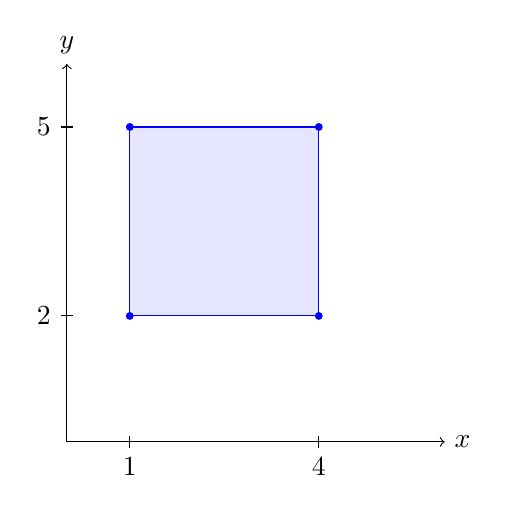
\begin{tikzpicture}[scale=0.8]
    % Eixos
    \draw[->] (0,0) -- (6,0) node[right] {$x$};
    \draw[->] (0,0) -- (0,6) node[above] {$y$};
    % Retângulo preenchido
    \filldraw[fill=blue!10,draw=blue] (1,2) rectangle (4,5);
    % Marcas nos eixos
    \foreach \x in {1,4}
        \draw (\x,0.1) -- (\x,-0.1) node[below] {\x};
    \foreach \y in {2,5}
        \draw (0.1,\y) -- (-0.1,\y) node[left] {\y};
    % Pontos dos vértices
    \foreach \x/\y in {1/2, 1/5, 4/2, 4/5}
        \filldraw[blue] (\x,\y) circle (1.5pt);
\end{tikzpicture}
\end{center}
}

\FloatBarrier

% Exercise ID: MAT_P4FUNCOE_0PX_IGX_002
% Created: 2025-11-26
% Difficulty: 2/5

\exercicio{
No plano cartesiano está desenhado o seguinte retângulo:

\begin{center}
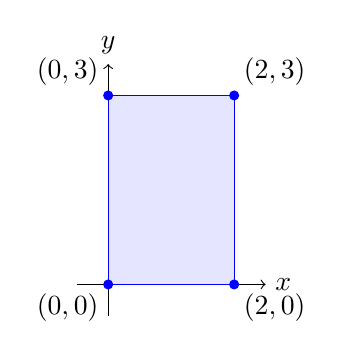
\begin{tikzpicture}[scale=0.8]
    % Eixos
    \draw[->] (-0.5,0) -- (2.5,0) node[right] {$x$};
    \draw[->] (0,-0.5) -- (0,3.5) node[above] {$y$};
    % Retângulo
    \draw[fill=blue!10,draw=blue] (0,0) rectangle (2,3);
    % Vértices
    \foreach \x/\y in {0/0, 0/3, 2/0, 2/3}
        \filldraw[blue] (\x,\y) circle (2pt);
    % Coordenadas dos vértices
    \node[below left] at (0,0) {$(0,0)$};
    \node[above left] at (0,3) {$(0,3)$};
    \node[below right] at (2,0) {$(2,0)$};
    \node[above right] at (2,3) {$(2,3)$};
\end{tikzpicture}
\end{center}

Indique o produto cartesiano de intervalos que corresponde ao conjunto de pontos do retângulo.
}

\FloatBarrier


\newpage

\section{1 - generalidades funcoes}

% Exercise ID: MAT_P4FUNCOE_1GX_ACA_001
% Created: 2025-11-28
% Difficulty: 3/5

\exercicio{Considere as seguintes afirmações sobre o preço p>0, a quantidade demandada q(p)\ge 0 e a despesa total D(p)=p\,q(p). Para cada afirmação: (i) classifique-a como "sempre verdadeira", "às vezes verdadeira" ou "falsa"; (ii) justifique brevemente a sua resposta (prova curta ou contraexemplo).

\begin{enumerate}[a)]
\item Quando o preço aumenta, a despesa total D(p) aumenta.
\item Se q(p) é decrescente em p, então D(p) é decrescente.
\item Se q(p)=k/p (k>0), então D(p) é constante e não depende de p.
\item Se p_1<p_2 e D(p_2)>D(p_1), então necessariamente q(p_2)>q(p_1).
\end{enumerate}}
\FloatBarrier

% Exercise ID: MAT_P4FUNCOE_1GX_ACX_001
% Created: 2025-11-28
% Difficulty: 3/5

\exercicio{'Considere as seguintes afirmações sobre preço (p)}

\FloatBarrier

% Exercise ID: MAT_P4FUNCOE_1GX_ACX_002
% Created: 2025-11-28
% Difficulty: 3/5

\exercicio{'Considere as seguintes afirmações sobre preço (p)}

\FloatBarrier

% Exercise ID: MAT_P4FUNCOE_1GFUN_AFC_001
% Module: MÓDULO P4 - Funções | Concept: Generalidades acerca de Funções
% Difficulty: 3/5 (Médio) | Format: desenvolvimento
% Tags: afirmacoes_causais, funcoes, relacoes_causais, analise_matematica
% Author: Professor | Date: 2025-11-28
% Status: active

\exercicio{Considere P (preço) e D (despesa) relacionadas por uma função D = f(P). Para cada uma das afirmações seguintes: (i) indique se é verdadeira ou falsa; (ii) justifique a sua resposta com argumentos matemáticos; (iii) quando possível, dê um exemplo explícito de função f que torne a afirmação verdadeira e outro que a torne falsa.
\par
\subexercicio{(A) "Quando o preço aumenta, a despesa aumenta."}
\subexercicio{(B) "Se o preço dobra, então a despesa dobra."}
\subexercicio{(C) "Se f for estritamente crescente, então qualquer aumento do preço implica um aumento da despesa."}
\subexercicio{(D) "Se f for constante, então a despesa não varia quando o preço varia."}}
\FloatBarrier

% Exercise ID: MAT_P4FUNCOE_1GX_ACD_001
% Created: 2025-11-27
% Difficulty: 3/5

\exercicio{Classifique V/F e justifique: (a) Quando o preço de um bem aumenta}

\FloatBarrier

% Exercise ID: MAT_P4FUNCOE_1GX_ACM_001
% Created: 2025-11-27
% Difficulty: 3/5

\exercicio{Classificação de afirmações: para cada afirmação indique VERDADEIRA/FALSA}

\FloatBarrier

% Exercise ID: MAT_P4FUNCOE_1GX_ACM_002
% Created: 2025-11-27
% Difficulty: 3/5

\exercicio{Teste de logging de inputs.}

\FloatBarrier

% Exercise ID: MAT_P4FUNCOE_1GX_ACR_001
% Created: 2025-11-27
% Difficulty: 3/5

\exercicio{Classifique as seguintes afirmações como VERDADEIRA ou FALSA; justifique rigorosamente e}

\FloatBarrier

% Exercise ID: MAT_P4FUNCOE_1GX_ACX_001
% Created: 2025-11-29
% Difficulty: 2/5

\exercicio{Teste de staging via wrapper}

\FloatBarrier

% Exercise ID: MAT_P4FUNCOE_1GX_ACX_001
% Created: 2025-11-27
% Difficulty: 2/5

\exercicio{Considere que}

\FloatBarrier

% Exercise ID: MAT_P4FUNCOE_1GEN_AR_001
% Created: 2025-11-27
% Difficulty: 2/5

\exercicio{Classifique cada afirmação como Verdadeira (V) ou Falsa (F) e justifique brevemente.}

\subexercicio{(a) Quando o preço de um bem aumenta, a despesa (gasto total) com esse bem aumenta.}

\subexercicio{(b) Se a quantidade consumida desse bem se mantém fixa, então um aumento do preço implica um aumento da despesa.}

\subexercicio{(c) A relação que associa a cada preço $p$ a despesa total $D(p)=p\cdot q(p)$ é, em toda situação, uma função (ou seja, a cada preço corresponde um único valor de despesa).}

\subexercicio{(d) Se $D(p)=p\cdot q(p)$ é uma função monótona crescente em $p$ (para $p>0$), então obrigatoriamente $q(p)$ é constante e positiva.}

\subexercicio{(e) Se $D(p)=p\cdot q(p)$ é injetora para $p>0$, então $q(p)$ é também uma função injetora.}

\FloatBarrier

% Exercise ID: MAT_P4FUNCOE_1GX_ARX_001
% Created: 2025-11-27
% Difficulty: 2/5

\exercicio{Teste de afirmação: 1+1=2}

\FloatBarrier

% Exercise ID: MAT_P4FUNCOE_1GX_ARX_002
% Created: 2025-11-27
% Difficulty: 2/5

\exercicio{Classifique cada uma das afirmações seguintes como Verdadeira (V) ou Falsa (F). Em cada caso, justifique brevemente a sua resposta.}

\subexercicio{(a) "Quando o preço de um produto aumenta, a despesa total com esse produto aumenta."}

\subexercicio{(b) "Se o preço de um produto aumenta e a quantidade vendida permanece exactamente a mesma, então a despesa total aumenta."}

\subexercicio{(c) "Se uma relação associa a cada preço uma despesa (ou seja, para cada preço existe exactamente uma despesa associada), então essa relação é uma função do conjunto dos preços no conjunto das despesas."}

\subexercicio{(d) "Se $f: \mathbb{R}\to\mathbb{R}$ é crescente, então para quaisquer $x_1<x_2$ temos $f(x_1)\le f(x_2)$."}

\subexercicio{(e) "Uma função que é injectiva garante que valores iguais da imagem correspondem a argumentos iguais."}
\FloatBarrier

% Exercise ID: MAT_P4FUNCOE_1GX_ARX_004
% Created: 2025-11-27
% Difficulty: 2/5

\exercicio{Quero que cries um exercício no módulo P4_funcoes na generalidades de funcoes (procurar nomenclatura) e adiciones um novo tipo de exercício (escolhe tu a nomenclatura do tipo de exercício!)}

\FloatBarrier

% Exercise ID: MAT_P4FUNCOE_1GX_ARX_005
% Created: 2025-11-27
% Difficulty: 2/5

\exercicio{Quero que cries um exercício no módulo P4_funcoes na generalidades de funcoes onde os alunos analisem afirmacoes tipo 'quando o preço aumenta a despesa vai aumentar'}

\FloatBarrier

% meta:
% id: MAT_P4FUNCOE_1GX_AVF_001
% title: "Afirmações sobre preço e despesa"
% difficulty: 2
% tags: ["afirmacoes","preco","despesa","verdadeiro_falso"]
% author: "OpenAI"
% has_parts: true
% parts_count: 3

\section{Afirmações sobre preço e despesa}

\exercicio{
Considere a seguinte situação:

Numa loja, o preço de um produto é representado por $p$ (em euros) e a despesa total dos clientes é dada por $D(p)$.

Para cada uma das afirmações seguintes, indique se é verdadeira ou falsa, justificando a sua resposta:
\begin{enumerate}
    \item Quando o preço aumenta, a despesa total $D(p)$ aumenta sempre.
    \item Se o preço for zero, a despesa total $D(0)$ é necessariamente zero.
    \item Se a despesa total $D(p)$ diminui quando o preço aumenta, então os clientes estão a comprar menos produtos.
\end{enumerate}
}

\FloatBarrier

% meta:
% id: MAT_P4FUNCOE_1GX_AAF_001
% title: "Análise de afirmações sobre preço e despesa"
% discipline: "matematica"
% module: "P4_funcoes"
% concept: "1-generalidades_funcoes"
% tipo: "analise_afirmacoes"
% difficulty: 2
% tags: "analise,afirmacoes,preco,despesa"
% author: "OpenAI"
% version: 1

\section{Análise de afirmações}

\exercicio{
Considere a seguinte situação:

"Numa loja, o preço de um produto é representado por $p$ (em euros) e a despesa total dos clientes é dada por $D(p)$.")

Para cada uma das afirmações seguintes, indique se é verdadeira ou falsa, justificando a sua resposta:
\begin{enumerate}
    \item Quando o preço aumenta, a despesa total $D(p)$ aumenta sempre.
    \item Se o preço for zero, a despesa total $D(0)$ é necessariamente zero.
    \item Se a despesa total $D(p)$ diminui quando o preço aumenta, então os clientes estão a comprar menos produtos.
\end{enumerate}
}

\FloatBarrier

% Exercise ID: MAT_P4FUNCOE_1GX_ICX_001
% Created: 2025-11-26
% Difficulty: 2/5

\exercicio{Considere a seguinte situação: Numa loja, o preço de um produto é representado por x (em euros) e a despesa total dos clientes é dada por D(x). Indique se as seguintes afirmações são verdadeiras ou falsas, justificando a sua resposta.}

\FloatBarrier

% Exercise ID: MAT_P4FUNCOE_1GX_ICX_002
% Created: 2025-11-26
% Difficulty: 2/5

\exercicio{AAAAAAAAAAAAAAAAAAAAAAAAAAAAAAAAAAAAAAAAAAAAAAAAAAAAAAAAAAAAAAAAAAAAAAAAAAAAAAAAAAAAAAAAAAAAAAAAAAAAAAAAAAAAAAAAAAAAAAAAAAAAAAAAAAAAAAAAAAAAAAAAAAAAAAAAAAAAAAAAAAAAAAAAAAAAAAAAAAAAAAAAAAAAAAAAAAAAAAAAAAAAAAAAAAAAAAAAAAAAAAAAAAAAAAAAAAAAAAAAAAAAAAAAAAAAAAAAAAAAAAAAAAAAAAAAAAAAAAAAAAAAAAAAAAAAAAAAAAAAAAAAAAAAAAAAAAAAAAAAAAAAAAAAAAAAAAAAAAAAAAAAAAAAAAAAAAAAAAAAAAAAAAAAAAAAAAAAAAAAAAAAAAAAAAAAAAAAAAAAAAAAAAAAAAAAAAAAAAAAAAAAAAAAAAAAAAAAAAAAAAAAAAAAAAAAAAAAAAAAAAAAAAAAAAAAAAAAAAAAAAAAAAAAAAAAAAAAAAAAAAAAAAAAAAAAAAAAAAAAAAAAAAAAAAAAAAAAAAAAAAAAAAAAAAAAAAAAAAAAAAAAAAAAAAAAAAAAAAAAAAAAAAAAAAAAAAAAAAAAAAAAAAAAAAAAAAAAAAAAAAAAAAAAAAAAAAAAAAAAAAAAAAAAAAAAAAAAAAAAAAAAAAAAAAAAAAAAAAAAAAAAAAAAAAAAAAAAAAAAAAAAAAAAAAAAAAAAAAAAAAAAAAAAAAAAAAAAAAAAAAAAAAAAAAAAAAAAAAAAAAAAAAAAAAAAAAAAAAAAAAAAAAAAAAAAAAAAAAAAAAAAAAAAAAAAAAAAAAAAAAAAAAAAAAAAAAAAAAAAAAAAAAAAAAAAAAAAAAAAAAAAAAAAAAAAAAAAAAAAAAAAAAAAAAAAAAAAAAAAAAAAAAAAAAAAAAAAAAAAAAAAAAAAAAAAAAAAAAAAAAAAAAAAAAAAAAAAAAAAAAAAAAAAAAAAAAAAAAAAAAAAAAAAAAAAAAAAAAAAAAAAAAAAAAAAAAAAAAAAAAAAAAAAAAAAAAAAAAAAAAAAAAAAAAAAAAAAAAAAAAAAAAAAAAAAAAAAAAAAAAAAAAAAAAAAAAAAAAAAAAAAAAAAAAAAAAAAAAAAAAAAAAAAAAAAAAAAAAAAAAAAAAAAAAAAAAAAAAAAAAAAAAAAAAAAAAAAAAAAAAAAAAAAAAAAAAAAAAAAAAAAAAAAAAAAAAAAAAAAAAAAAAAAAAAAAAAAAAAAAAAAAAAAAAAAAAAAAAAAAAAAAAAAAAAAAAAAAAAAAAAAAAAAAAAAAAAAAAAAAAAAAAAAAAAAAAAAAAAAAAAAAAAAAAAAAAAAAAAAAAAAAAAAAAAAAAAAAAAAAAAAAAAAAAAAAAAAAAAAAAAAAAAAAAAAAAAAAAAAAAAAAAAAAAAAAAAAAAAAAAAAAAAAAAAAAAAAAAAAAAAAAAAAAAAAAAAAAAAAAAAAAAAAAAAAAAAAAAAAAAAAAAAAAAAAAAAAAAAAAAAAAAAAAAAAAAAAAAAAAAAAAAAAAAAAAAAAAAAAAAAAAAAAAAAAAAAAAAAAAAAAAAAAAAAAAAAAAAAAAAAAAAAAAAAAAAAAAAAAAAAAAAAAAAAAAAAAAAAAAAAAAAAAAAAAAAAAAAAAAAAAAAAAAAAAAAAAAAAAAAAAAAAAAAAAAAAAAAAAAAAAAAAAAAAAAAAAAAAAAAAAAAAAAAAAAAAAAAAAAAAAAAAAAAAAAAAAAAAAAAAAAAAAAAAAAAAAAAAAAAAAAAAAAAAAAAAAAAAAAAAAAAAAAAAAAAAAAAAAAAAAAAAAAAAAAAAAAAAAAAAAAAAAAAAAAAAAAAAAAAAAAAAAAAAAAAAAAAAAAAAAAAAAAAAAAAAAAAAAAAAAAAAAAAAAAAAAAAAAAAAAAAAAAAAAAAAAAAAAAAAAAAAAAAAAAAAAAAAAAAAAAAAAAAAAAAAAAAAAAAAAAAAAAAAAAAAAAAAAAAAAAAAAAAAAAAAAAAAA}

\FloatBarrier

% Exercise ID: MAT_P4FUNCOE_1GX_ICX_003
% Created: 2025-11-26
% Difficulty: 2/5

\exercicio{Questão com caracteres especiais: % $ & { } [ ] ~ # _ ^ \}

\FloatBarrier

% Exercise ID: MAT_P4FUNCOE_1GX_ICX_004
% Created: 2025-11-26
% Difficulty: 2/5

\exercicio{Considere a seguinte situação: Numa loja, o preço de um produto é representado por x (em euros) e a despesa total dos clientes é dada por D(x). Indique se as seguintes afirmações são verdadeiras ou falsas, justificando a sua resposta.\par 1. Quando o preço aumenta, a despesa total D(x) aumenta sempre.\par 2. Se o preço for zero, a despesa total D(0) é necessariamente zero.\par 3. Se a despesa total D(x) diminui quando o preço aumenta, então os clientes estão a comprar menos produtos.}

\FloatBarrier

% Exercise ID: MAT_P4FUNCOE_1GX_ICX_005
% Created: 2025-11-26
% Difficulty: 2/5

\exercicio{Questão com caracteres especiais: % $ & { } [ ] ~ # _ ^ \}

\FloatBarrier

% Exercise ID: MAT_P4FUNCOE_1GX_ICX_006
% Created: 2025-11-26
% Difficulty: 2/5

\exercicio{A*3000}

\FloatBarrier

% Exercise ID: MAT_P4FUNCOE_1GX_ICX_007
% Created: 2025-11-26
% Difficulty: 2/5

\exercicio{Quando o preço aumenta, a despesa aumenta? Verdadeiro ou falso? Justifique.}

\FloatBarrier

% Exercise ID: MAT_P4FUNCOE_1GX_ICX_008
% Created: 2025-11-27
% Difficulty: 2/5

\exercicio{Considere a seguinte situação: Numa loja, o preço de um produto é representado por x (em euros) e a despesa total dos clientes é dada por D(x). Indique se as seguintes afirmações são verdadeiras ou falsas, justificando a sua resposta.}

\FloatBarrier

% Exercise ID: MAT_P4FUNCOE_1GX_ICX_009
% Created: 2025-11-27
% Difficulty: 2/5

\exercicio{AAAAAAAAAAAAAAAAAAAAAAAAAAAAAAAAAAAAAAAAAAAAAAAAAAAAAAAAAAAAAAAAAAAAAAAAAAAAAAAAAAAAAAAAAAAAAAAAAAAAAAAAAAAAAAAAAAAAAAAAAAAAAAAAAAAAAAAAAAAAAAAAAAAAAAAAAAAAAAAAAAAAAAAAAAAAAAAAAAAAAAAAAAAAAAAAAAAAAAAAAAAAAAAAAAAAAAAAAAAAAAAAAAAAAAAAAAAAAAAAAAAAAAAAAAAAAAAAAAAAAAAAAAAAAAAAAAAAAAAAAAAAAAAAAAAAAAAAAAAAAAAAAAAAAAAAAAAAAAAAAAAAAAAAAAAAAAAAAAAAAAAAAAAAAAAAAAAAAAAAAAAAAAAAAAAAAAAAAAAAAAAAAAAAAAAAAAAAAAAAAAAAAAAAAAAAAAAAAAAAAAAAAAAAAAAAAAAAAAAAAAAAAAAAAAAAAAAAAAAAAAAAAAAAAAAAAAAAAAAAAAAAAAAAAAAAAAAAAAAAAAAAAAAAAAAAAAAAAAAAAAAAAAAAAAAAAAAAAAAAAAAAAAAAAAAAAAAAAAAAAAAAAAAAAAAAAAAAAAAAAAAAAAAAAAAAAAAAAAAAAAAAAAAAAAAAAAAAAAAAAAAAAAAAAAAAAAAAAAAAAAAAAAAAAAAAAAAAAAAAAAAAAAAAAAAAAAAAAAAAAAAAAAAAAAAAAAAAAAAAAAAAAAAAAAAAAAAAAAAAAAAAAAAAAAAAAAAAAAAAAAAAAAAAAAAAAAAAAAAAAAAAAAAAAAAAAAAAAAAAAAAAAAAAAAAAAAAAAAAAAAAAAAAAAAAAAAAAAAAAAAAAAAAAAAAAAAAAAAAAAAAAAAAAAAAAAAAAAAAAAAAAAAAAAAAAAAAAAAAAAAAAAAAAAAAAAAAAAAAAAAAAAAAAAAAAAAAAAAAAAAAAAAAAAAAAAAAAAAAAAAAAAAAAAAAAAAAAAAAAAAAAAAAAAAAAAAAAAAAAAAAAAAAAAAAAAAAAAAAAAAAAAAAAAAAAAAAAAAAAAAAAAAAAAAAAAAAAAAAAAAAAAAAAAAAAAAAAAAAAAAAAAAAAAAAAAAAAAAAAAAAAAAAAAAAAAAAAAAAAAAAAAAAAAAAAAAAAAAAAAAAAAAAAAAAAAAAAAAAAAAAAAAAAAAAAAAAAAAAAAAAAAAAAAAAAAAAAAAAAAAAAAAAAAAAAAAAAAAAAAAAAAAAAAAAAAAAAAAAAAAAAAAAAAAAAAAAAAAAAAAAAAAAAAAAAAAAAAAAAAAAAAAAAAAAAAAAAAAAAAAAAAAAAAAAAAAAAAAAAAAAAAAAAAAAAAAAAAAAAAAAAAAAAAAAAAAAAAAAAAAAAAAAAAAAAAAAAAAAAAAAAAAAAAAAAAAAAAAAAAAAAAAAAAAAAAAAAAAAAAAAAAAAAAAAAAAAAAAAAAAAAAAAAAAAAAAAAAAAAAAAAAAAAAAAAAAAAAAAAAAAAAAAAAAAAAAAAAAAAAAAAAAAAAAAAAAAAAAAAAAAAAAAAAAAAAAAAAAAAAAAAAAAAAAAAAAAAAAAAAAAAAAAAAAAAAAAAAAAAAAAAAAAAAAAAAAAAAAAAAAAAAAAAAAAAAAAAAAAAAAAAAAAAAAAAAAAAAAAAAAAAAAAAAAAAAAAAAAAAAAAAAAAAAAAAAAAAAAAAAAAAAAAAAAAAAAAAAAAAAAAAAAAAAAAAAAAAAAAAAAAAAAAAAAAAAAAAAAAAAAAAAAAAAAAAAAAAAAAAAAAAAAAAAAAAAAAAAAAAAAAAAAAAAAAAAAAAAAAAAAAAAAAAAAAAAAAAAAAAAAAAAAAAAAAAAAAAAAAAAAAAAAAAAAAAAAAAAAAAAAAAAAAAAAAAAAAAAAAAAAAAAAAAAAAAAAAAAAAAAAAAAAAAAAAAAAAAAAAAAAAAAAAAAAAAAAAAAAAAAAAAAAAAAAAAAAAAAAAAAAAAAAAAAAAAAAAAAAAAAAAAAAAAAAAAAAAAAAAAAAAAAAAAAAAAAAAAAAAA}

\FloatBarrier

% Exercise ID: MAT_P4FUNCOE_1GX_ICX_010
% Created: 2025-11-27
% Difficulty: 2/5

\exercicio{Questão com caracteres especiais: % $ & { } [ ] ~ # _ ^ \}

\FloatBarrier

% Exercise ID: MAT_P4FUNCOE_1GX_ICX_011
% Created: 2025-11-27
% Difficulty: 2/5

\exercicio{Considere a seguinte situação: Numa loja, o preço de um produto é representado por x (em euros) e a despesa total dos clientes é dada por D(x). Indique se as seguintes afirmações são verdadeiras ou falsas, justificando a sua resposta.}

\FloatBarrier

% Exercise ID: MAT_P4FUNCOE_1GX_ICX_012
% Created: 2025-11-27
% Difficulty: 2/5

\exercicio{AAAAAAAAAAAAAAAAAAAAAAAAAAAAAAAAAAAAAAAAAAAAAAAAAAAAAAAAAAAAAAAAAAAAAAAAAAAAAAAAAAAAAAAAAAAAAAAAAAAAAAAAAAAAAAAAAAAAAAAAAAAAAAAAAAAAAAAAAAAAAAAAAAAAAAAAAAAAAAAAAAAAAAAAAAAAAAAAAAAAAAAAAAAAAAAAAAAAAAAAAAAAAAAAAAAAAAAAAAAAAAAAAAAAAAAAAAAAAAAAAAAAAAAAAAAAAAAAAAAAAAAAAAAAAAAAAAAAAAAAAAAAAAAAAAAAAAAAAAAAAAAAAAAAAAAAAAAAAAAAAAAAAAAAAAAAAAAAAAAAAAAAAAAAAAAAAAAAAAAAAAAAAAAAAAAAAAAAAAAAAAAAAAAAAAAAAAAAAAAAAAAAAAAAAAAAAAAAAAAAAAAAAAAAAAAAAAAAAAAAAAAAAAAAAAAAAAAAAAAAAAAAAAAAAAAAAAAAAAAAAAAAAAAAAAAAAAAAAAAAAAAAAAAAAAAAAAAAAAAAAAAAAAAAAAAAAAAAAAAAAAAAAAAAAAAAAAAAAAAAAAAAAAAAAAAAAAAAAAAAAAAAAAAAAAAAAAAAAAAAAAAAAAAAAAAAAAAAAAAAAAAAAAAAAAAAAAAAAAAAAAAAAAAAAAAAAAAAAAAAAAAAAAAAAAAAAAAAAAAAAAAAAAAAAAAAAAAAAAAAAAAAAAAAAAAAAAAAAAAAAAAAAAAAAAAAAAAAAAAAAAAAAAAAAAAAAAAAAAAAAAAAAAAAAAAAAAAAAAAAAAAAAAAAAAAAAAAAAAAAAAAAAAAAAAAAAAAAAAAAAAAAAAAAAAAAAAAAAAAAAAAAAAAAAAAAAAAAAAAAAAAAAAAAAAAAAAAAAAAAAAAAAAAAAAAAAAAAAAAAAAAAAAAAAAAAAAAAAAAAAAAAAAAAAAAAAAAAAAAAAAAAAAAAAAAAAAAAAAAAAAAAAAAAAAAAAAAAAAAAAAAAAAAAAAAAAAAAAAAAAAAAAAAAAAAAAAAAAAAAAAAAAAAAAAAAAAAAAAAAAAAAAAAAAAAAAAAAAAAAAAAAAAAAAAAAAAAAAAAAAAAAAAAAAAAAAAAAAAAAAAAAAAAAAAAAAAAAAAAAAAAAAAAAAAAAAAAAAAAAAAAAAAAAAAAAAAAAAAAAAAAAAAAAAAAAAAAAAAAAAAAAAAAAAAAAAAAAAAAAAAAAAAAAAAAAAAAAAAAAAAAAAAAAAAAAAAAAAAAAAAAAAAAAAAAAAAAAAAAAAAAAAAAAAAAAAAAAAAAAAAAAAAAAAAAAAAAAAAAAAAAAAAAAAAAAAAAAAAAAAAAAAAAAAAAAAAAAAAAAAAAAAAAAAAAAAAAAAAAAAAAAAAAAAAAAAAAAAAAAAAAAAAAAAAAAAAAAAAAAAAAAAAAAAAAAAAAAAAAAAAAAAAAAAAAAAAAAAAAAAAAAAAAAAAAAAAAAAAAAAAAAAAAAAAAAAAAAAAAAAAAAAAAAAAAAAAAAAAAAAAAAAAAAAAAAAAAAAAAAAAAAAAAAAAAAAAAAAAAAAAAAAAAAAAAAAAAAAAAAAAAAAAAAAAAAAAAAAAAAAAAAAAAAAAAAAAAAAAAAAAAAAAAAAAAAAAAAAAAAAAAAAAAAAAAAAAAAAAAAAAAAAAAAAAAAAAAAAAAAAAAAAAAAAAAAAAAAAAAAAAAAAAAAAAAAAAAAAAAAAAAAAAAAAAAAAAAAAAAAAAAAAAAAAAAAAAAAAAAAAAAAAAAAAAAAAAAAAAAAAAAAAAAAAAAAAAAAAAAAAAAAAAAAAAAAAAAAAAAAAAAAAAAAAAAAAAAAAAAAAAAAAAAAAAAAAAAAAAAAAAAAAAAAAAAAAAAAAAAAAAAAAAAAAAAAAAAAAAAAAAAAAAAAAAAAAAAAAAAAAAAAAAAAAAAAAAAAAAAAAAAAAAAAAAAAAAAAAAAAAAAAAAAAAAAAAAAAAAAAAAAAAAAAAAAAAAAAAAAAAAAAAAAAAAAAAAAAAAAA}

\FloatBarrier

% Exercise ID: MAT_P4FUNCOE_1GX_ICX_013
% Created: 2025-11-27
% Difficulty: 2/5

\exercicio{Questão com caracteres especiais: % $ & { } [ ] ~ # _ ^ \}

\FloatBarrier

% Exercise ID: MAT_P4FUNCOE_1GX_ICX_014
% Created: 2025-11-27
% Difficulty: 2/5

\exercicio{Considere a seguinte situação: Numa loja, o preço de um produto é representado por x (em euros) e a despesa total dos clientes é dada por D(x). Indique se as seguintes afirmações são verdadeiras ou falsas, justificando a sua resposta.}

\FloatBarrier

% Exercise ID: MAT_P4FUNCOE_1GX_ICX_015
% Created: 2025-11-27
% Difficulty: 2/5

\exercicio{AAAAAAAAAAAAAAAAAAAAAAAAAAAAAAAAAAAAAAAAAAAAAAAAAAAAAAAAAAAAAAAAAAAAAAAAAAAAAAAAAAAAAAAAAAAAAAAAAAAAAAAAAAAAAAAAAAAAAAAAAAAAAAAAAAAAAAAAAAAAAAAAAAAAAAAAAAAAAAAAAAAAAAAAAAAAAAAAAAAAAAAAAAAAAAAAAAAAAAAAAAAAAAAAAAAAAAAAAAAAAAAAAAAAAAAAAAAAAAAAAAAAAAAAAAAAAAAAAAAAAAAAAAAAAAAAAAAAAAAAAAAAAAAAAAAAAAAAAAAAAAAAAAAAAAAAAAAAAAAAAAAAAAAAAAAAAAAAAAAAAAAAAAAAAAAAAAAAAAAAAAAAAAAAAAAAAAAAAAAAAAAAAAAAAAAAAAAAAAAAAAAAAAAAAAAAAAAAAAAAAAAAAAAAAAAAAAAAAAAAAAAAAAAAAAAAAAAAAAAAAAAAAAAAAAAAAAAAAAAAAAAAAAAAAAAAAAAAAAAAAAAAAAAAAAAAAAAAAAAAAAAAAAAAAAAAAAAAAAAAAAAAAAAAAAAAAAAAAAAAAAAAAAAAAAAAAAAAAAAAAAAAAAAAAAAAAAAAAAAAAAAAAAAAAAAAAAAAAAAAAAAAAAAAAAAAAAAAAAAAAAAAAAAAAAAAAAAAAAAAAAAAAAAAAAAAAAAAAAAAAAAAAAAAAAAAAAAAAAAAAAAAAAAAAAAAAAAAAAAAAAAAAAAAAAAAAAAAAAAAAAAAAAAAAAAAAAAAAAAAAAAAAAAAAAAAAAAAAAAAAAAAAAAAAAAAAAAAAAAAAAAAAAAAAAAAAAAAAAAAAAAAAAAAAAAAAAAAAAAAAAAAAAAAAAAAAAAAAAAAAAAAAAAAAAAAAAAAAAAAAAAAAAAAAAAAAAAAAAAAAAAAAAAAAAAAAAAAAAAAAAAAAAAAAAAAAAAAAAAAAAAAAAAAAAAAAAAAAAAAAAAAAAAAAAAAAAAAAAAAAAAAAAAAAAAAAAAAAAAAAAAAAAAAAAAAAAAAAAAAAAAAAAAAAAAAAAAAAAAAAAAAAAAAAAAAAAAAAAAAAAAAAAAAAAAAAAAAAAAAAAAAAAAAAAAAAAAAAAAAAAAAAAAAAAAAAAAAAAAAAAAAAAAAAAAAAAAAAAAAAAAAAAAAAAAAAAAAAAAAAAAAAAAAAAAAAAAAAAAAAAAAAAAAAAAAAAAAAAAAAAAAAAAAAAAAAAAAAAAAAAAAAAAAAAAAAAAAAAAAAAAAAAAAAAAAAAAAAAAAAAAAAAAAAAAAAAAAAAAAAAAAAAAAAAAAAAAAAAAAAAAAAAAAAAAAAAAAAAAAAAAAAAAAAAAAAAAAAAAAAAAAAAAAAAAAAAAAAAAAAAAAAAAAAAAAAAAAAAAAAAAAAAAAAAAAAAAAAAAAAAAAAAAAAAAAAAAAAAAAAAAAAAAAAAAAAAAAAAAAAAAAAAAAAAAAAAAAAAAAAAAAAAAAAAAAAAAAAAAAAAAAAAAAAAAAAAAAAAAAAAAAAAAAAAAAAAAAAAAAAAAAAAAAAAAAAAAAAAAAAAAAAAAAAAAAAAAAAAAAAAAAAAAAAAAAAAAAAAAAAAAAAAAAAAAAAAAAAAAAAAAAAAAAAAAAAAAAAAAAAAAAAAAAAAAAAAAAAAAAAAAAAAAAAAAAAAAAAAAAAAAAAAAAAAAAAAAAAAAAAAAAAAAAAAAAAAAAAAAAAAAAAAAAAAAAAAAAAAAAAAAAAAAAAAAAAAAAAAAAAAAAAAAAAAAAAAAAAAAAAAAAAAAAAAAAAAAAAAAAAAAAAAAAAAAAAAAAAAAAAAAAAAAAAAAAAAAAAAAAAAAAAAAAAAAAAAAAAAAAAAAAAAAAAAAAAAAAAAAAAAAAAAAAAAAAAAAAAAAAAAAAAAAAAAAAAAAAAAAAAAAAAAAAAAAAAAAAAAAAAAAAAAAAAAAAAAAAAAAAAAAAAAAAAAAAAAAAAAAAAAAAAAAAAAAAAAAAAAAAAAAAAAAAAAAAAAAAAAAA}

\FloatBarrier

% Exercise ID: MAT_P4FUNCOE_1GX_ICX_016
% Created: 2025-11-27
% Difficulty: 2/5

\exercicio{Questão com caracteres especiais: % $ & { } [ ] ~ # _ ^ \}

\FloatBarrier

% Exercise ID: MAT_P4FUNCOE_1GX_ICX_017
% Created: 2025-11-27
% Difficulty: 2/5

\exercicio{Considere a seguinte situação: Numa loja, o preço de um produto é representado por x (em euros) e a despesa total dos clientes é dada por D(x). Indique se as seguintes afirmações são verdadeiras ou falsas, justificando a sua resposta.}

\FloatBarrier

% Exercise ID: MAT_P4FUNCOE_1GX_ICX_018
% Created: 2025-11-27
% Difficulty: 2/5

\exercicio{AAAAAAAAAAAAAAAAAAAAAAAAAAAAAAAAAAAAAAAAAAAAAAAAAAAAAAAAAAAAAAAAAAAAAAAAAAAAAAAAAAAAAAAAAAAAAAAAAAAAAAAAAAAAAAAAAAAAAAAAAAAAAAAAAAAAAAAAAAAAAAAAAAAAAAAAAAAAAAAAAAAAAAAAAAAAAAAAAAAAAAAAAAAAAAAAAAAAAAAAAAAAAAAAAAAAAAAAAAAAAAAAAAAAAAAAAAAAAAAAAAAAAAAAAAAAAAAAAAAAAAAAAAAAAAAAAAAAAAAAAAAAAAAAAAAAAAAAAAAAAAAAAAAAAAAAAAAAAAAAAAAAAAAAAAAAAAAAAAAAAAAAAAAAAAAAAAAAAAAAAAAAAAAAAAAAAAAAAAAAAAAAAAAAAAAAAAAAAAAAAAAAAAAAAAAAAAAAAAAAAAAAAAAAAAAAAAAAAAAAAAAAAAAAAAAAAAAAAAAAAAAAAAAAAAAAAAAAAAAAAAAAAAAAAAAAAAAAAAAAAAAAAAAAAAAAAAAAAAAAAAAAAAAAAAAAAAAAAAAAAAAAAAAAAAAAAAAAAAAAAAAAAAAAAAAAAAAAAAAAAAAAAAAAAAAAAAAAAAAAAAAAAAAAAAAAAAAAAAAAAAAAAAAAAAAAAAAAAAAAAAAAAAAAAAAAAAAAAAAAAAAAAAAAAAAAAAAAAAAAAAAAAAAAAAAAAAAAAAAAAAAAAAAAAAAAAAAAAAAAAAAAAAAAAAAAAAAAAAAAAAAAAAAAAAAAAAAAAAAAAAAAAAAAAAAAAAAAAAAAAAAAAAAAAAAAAAAAAAAAAAAAAAAAAAAAAAAAAAAAAAAAAAAAAAAAAAAAAAAAAAAAAAAAAAAAAAAAAAAAAAAAAAAAAAAAAAAAAAAAAAAAAAAAAAAAAAAAAAAAAAAAAAAAAAAAAAAAAAAAAAAAAAAAAAAAAAAAAAAAAAAAAAAAAAAAAAAAAAAAAAAAAAAAAAAAAAAAAAAAAAAAAAAAAAAAAAAAAAAAAAAAAAAAAAAAAAAAAAAAAAAAAAAAAAAAAAAAAAAAAAAAAAAAAAAAAAAAAAAAAAAAAAAAAAAAAAAAAAAAAAAAAAAAAAAAAAAAAAAAAAAAAAAAAAAAAAAAAAAAAAAAAAAAAAAAAAAAAAAAAAAAAAAAAAAAAAAAAAAAAAAAAAAAAAAAAAAAAAAAAAAAAAAAAAAAAAAAAAAAAAAAAAAAAAAAAAAAAAAAAAAAAAAAAAAAAAAAAAAAAAAAAAAAAAAAAAAAAAAAAAAAAAAAAAAAAAAAAAAAAAAAAAAAAAAAAAAAAAAAAAAAAAAAAAAAAAAAAAAAAAAAAAAAAAAAAAAAAAAAAAAAAAAAAAAAAAAAAAAAAAAAAAAAAAAAAAAAAAAAAAAAAAAAAAAAAAAAAAAAAAAAAAAAAAAAAAAAAAAAAAAAAAAAAAAAAAAAAAAAAAAAAAAAAAAAAAAAAAAAAAAAAAAAAAAAAAAAAAAAAAAAAAAAAAAAAAAAAAAAAAAAAAAAAAAAAAAAAAAAAAAAAAAAAAAAAAAAAAAAAAAAAAAAAAAAAAAAAAAAAAAAAAAAAAAAAAAAAAAAAAAAAAAAAAAAAAAAAAAAAAAAAAAAAAAAAAAAAAAAAAAAAAAAAAAAAAAAAAAAAAAAAAAAAAAAAAAAAAAAAAAAAAAAAAAAAAAAAAAAAAAAAAAAAAAAAAAAAAAAAAAAAAAAAAAAAAAAAAAAAAAAAAAAAAAAAAAAAAAAAAAAAAAAAAAAAAAAAAAAAAAAAAAAAAAAAAAAAAAAAAAAAAAAAAAAAAAAAAAAAAAAAAAAAAAAAAAAAAAAAAAAAAAAAAAAAAAAAAAAAAAAAAAAAAAAAAAAAAAAAAAAAAAAAAAAAAAAAAAAAAAAAAAAAAAAAAAAAAAAAAAAAAAAAAAAAAAAAAAAAAAAAAAAAAAAAAAAAAAAAAAAAAAAAAAAAAAAAAAAAAAAAAAAAAAAAAAAAAAAAAAAAAAAAAAAAAAAAAAA}

\FloatBarrier

% Exercise ID: MAT_P4FUNCOE_1GX_ICX_019
% Created: 2025-11-27
% Difficulty: 2/5

\exercicio{Questão com caracteres especiais: % $ & { } [ ] ~ # _ ^ \}

\FloatBarrier

% Exercise ID: MAT_P4FUNCOE_1GX_ICX_020
% Created: 2025-11-27
% Difficulty: 2/5

\exercicio{Considere a seguinte situação: Numa loja, o preço de um produto é representado por x (em euros) e a despesa total dos clientes é dada por D(x). Indique se as seguintes afirmações são verdadeiras ou falsas, justificando a sua resposta.}

\FloatBarrier

% Exercise ID: MAT_P4FUNCOE_1GX_ICX_021
% Created: 2025-11-27
% Difficulty: 2/5

\exercicio{AAAAAAAAAAAAAAAAAAAAAAAAAAAAAAAAAAAAAAAAAAAAAAAAAAAAAAAAAAAAAAAAAAAAAAAAAAAAAAAAAAAAAAAAAAAAAAAAAAAAAAAAAAAAAAAAAAAAAAAAAAAAAAAAAAAAAAAAAAAAAAAAAAAAAAAAAAAAAAAAAAAAAAAAAAAAAAAAAAAAAAAAAAAAAAAAAAAAAAAAAAAAAAAAAAAAAAAAAAAAAAAAAAAAAAAAAAAAAAAAAAAAAAAAAAAAAAAAAAAAAAAAAAAAAAAAAAAAAAAAAAAAAAAAAAAAAAAAAAAAAAAAAAAAAAAAAAAAAAAAAAAAAAAAAAAAAAAAAAAAAAAAAAAAAAAAAAAAAAAAAAAAAAAAAAAAAAAAAAAAAAAAAAAAAAAAAAAAAAAAAAAAAAAAAAAAAAAAAAAAAAAAAAAAAAAAAAAAAAAAAAAAAAAAAAAAAAAAAAAAAAAAAAAAAAAAAAAAAAAAAAAAAAAAAAAAAAAAAAAAAAAAAAAAAAAAAAAAAAAAAAAAAAAAAAAAAAAAAAAAAAAAAAAAAAAAAAAAAAAAAAAAAAAAAAAAAAAAAAAAAAAAAAAAAAAAAAAAAAAAAAAAAAAAAAAAAAAAAAAAAAAAAAAAAAAAAAAAAAAAAAAAAAAAAAAAAAAAAAAAAAAAAAAAAAAAAAAAAAAAAAAAAAAAAAAAAAAAAAAAAAAAAAAAAAAAAAAAAAAAAAAAAAAAAAAAAAAAAAAAAAAAAAAAAAAAAAAAAAAAAAAAAAAAAAAAAAAAAAAAAAAAAAAAAAAAAAAAAAAAAAAAAAAAAAAAAAAAAAAAAAAAAAAAAAAAAAAAAAAAAAAAAAAAAAAAAAAAAAAAAAAAAAAAAAAAAAAAAAAAAAAAAAAAAAAAAAAAAAAAAAAAAAAAAAAAAAAAAAAAAAAAAAAAAAAAAAAAAAAAAAAAAAAAAAAAAAAAAAAAAAAAAAAAAAAAAAAAAAAAAAAAAAAAAAAAAAAAAAAAAAAAAAAAAAAAAAAAAAAAAAAAAAAAAAAAAAAAAAAAAAAAAAAAAAAAAAAAAAAAAAAAAAAAAAAAAAAAAAAAAAAAAAAAAAAAAAAAAAAAAAAAAAAAAAAAAAAAAAAAAAAAAAAAAAAAAAAAAAAAAAAAAAAAAAAAAAAAAAAAAAAAAAAAAAAAAAAAAAAAAAAAAAAAAAAAAAAAAAAAAAAAAAAAAAAAAAAAAAAAAAAAAAAAAAAAAAAAAAAAAAAAAAAAAAAAAAAAAAAAAAAAAAAAAAAAAAAAAAAAAAAAAAAAAAAAAAAAAAAAAAAAAAAAAAAAAAAAAAAAAAAAAAAAAAAAAAAAAAAAAAAAAAAAAAAAAAAAAAAAAAAAAAAAAAAAAAAAAAAAAAAAAAAAAAAAAAAAAAAAAAAAAAAAAAAAAAAAAAAAAAAAAAAAAAAAAAAAAAAAAAAAAAAAAAAAAAAAAAAAAAAAAAAAAAAAAAAAAAAAAAAAAAAAAAAAAAAAAAAAAAAAAAAAAAAAAAAAAAAAAAAAAAAAAAAAAAAAAAAAAAAAAAAAAAAAAAAAAAAAAAAAAAAAAAAAAAAAAAAAAAAAAAAAAAAAAAAAAAAAAAAAAAAAAAAAAAAAAAAAAAAAAAAAAAAAAAAAAAAAAAAAAAAAAAAAAAAAAAAAAAAAAAAAAAAAAAAAAAAAAAAAAAAAAAAAAAAAAAAAAAAAAAAAAAAAAAAAAAAAAAAAAAAAAAAAAAAAAAAAAAAAAAAAAAAAAAAAAAAAAAAAAAAAAAAAAAAAAAAAAAAAAAAAAAAAAAAAAAAAAAAAAAAAAAAAAAAAAAAAAAAAAAAAAAAAAAAAAAAAAAAAAAAAAAAAAAAAAAAAAAAAAAAAAAAAAAAAAAAAAAAAAAAAAAAAAAAAAAAAAAAAAAAAAAAAAAAAAAAAAAAAAAAAAAAAAAAAAAAAAAAAAAAAAAAAAAAAAAAAAAAAAAAAAAAAAAAAAAAAAAAAAAAAAAAAAAAAAAAA}

\FloatBarrier

% Exercise ID: MAT_P4FUNCOE_1GX_ICX_022
% Created: 2025-11-27
% Difficulty: 2/5

\exercicio{Questão com caracteres especiais: % $ & { } [ ] ~ # _ ^ \}

\FloatBarrier

% Exercise ID: MAT_P4FUNCOE_1GX_ICX_023
% Created: 2025-11-27
% Difficulty: 2/5

\exercicio{Considere a seguinte situação: Numa loja, o preço de um produto é representado por x (em euros) e a despesa total dos clientes é dada por D(x). Indique se as seguintes afirmações são verdadeiras ou falsas, justificando a sua resposta.}

\FloatBarrier

% Exercise ID: MAT_P4FUNCOE_1GX_ICX_024
% Created: 2025-11-27
% Difficulty: 2/5

\exercicio{AAAAAAAAAAAAAAAAAAAAAAAAAAAAAAAAAAAAAAAAAAAAAAAAAAAAAAAAAAAAAAAAAAAAAAAAAAAAAAAAAAAAAAAAAAAAAAAAAAAAAAAAAAAAAAAAAAAAAAAAAAAAAAAAAAAAAAAAAAAAAAAAAAAAAAAAAAAAAAAAAAAAAAAAAAAAAAAAAAAAAAAAAAAAAAAAAAAAAAAAAAAAAAAAAAAAAAAAAAAAAAAAAAAAAAAAAAAAAAAAAAAAAAAAAAAAAAAAAAAAAAAAAAAAAAAAAAAAAAAAAAAAAAAAAAAAAAAAAAAAAAAAAAAAAAAAAAAAAAAAAAAAAAAAAAAAAAAAAAAAAAAAAAAAAAAAAAAAAAAAAAAAAAAAAAAAAAAAAAAAAAAAAAAAAAAAAAAAAAAAAAAAAAAAAAAAAAAAAAAAAAAAAAAAAAAAAAAAAAAAAAAAAAAAAAAAAAAAAAAAAAAAAAAAAAAAAAAAAAAAAAAAAAAAAAAAAAAAAAAAAAAAAAAAAAAAAAAAAAAAAAAAAAAAAAAAAAAAAAAAAAAAAAAAAAAAAAAAAAAAAAAAAAAAAAAAAAAAAAAAAAAAAAAAAAAAAAAAAAAAAAAAAAAAAAAAAAAAAAAAAAAAAAAAAAAAAAAAAAAAAAAAAAAAAAAAAAAAAAAAAAAAAAAAAAAAAAAAAAAAAAAAAAAAAAAAAAAAAAAAAAAAAAAAAAAAAAAAAAAAAAAAAAAAAAAAAAAAAAAAAAAAAAAAAAAAAAAAAAAAAAAAAAAAAAAAAAAAAAAAAAAAAAAAAAAAAAAAAAAAAAAAAAAAAAAAAAAAAAAAAAAAAAAAAAAAAAAAAAAAAAAAAAAAAAAAAAAAAAAAAAAAAAAAAAAAAAAAAAAAAAAAAAAAAAAAAAAAAAAAAAAAAAAAAAAAAAAAAAAAAAAAAAAAAAAAAAAAAAAAAAAAAAAAAAAAAAAAAAAAAAAAAAAAAAAAAAAAAAAAAAAAAAAAAAAAAAAAAAAAAAAAAAAAAAAAAAAAAAAAAAAAAAAAAAAAAAAAAAAAAAAAAAAAAAAAAAAAAAAAAAAAAAAAAAAAAAAAAAAAAAAAAAAAAAAAAAAAAAAAAAAAAAAAAAAAAAAAAAAAAAAAAAAAAAAAAAAAAAAAAAAAAAAAAAAAAAAAAAAAAAAAAAAAAAAAAAAAAAAAAAAAAAAAAAAAAAAAAAAAAAAAAAAAAAAAAAAAAAAAAAAAAAAAAAAAAAAAAAAAAAAAAAAAAAAAAAAAAAAAAAAAAAAAAAAAAAAAAAAAAAAAAAAAAAAAAAAAAAAAAAAAAAAAAAAAAAAAAAAAAAAAAAAAAAAAAAAAAAAAAAAAAAAAAAAAAAAAAAAAAAAAAAAAAAAAAAAAAAAAAAAAAAAAAAAAAAAAAAAAAAAAAAAAAAAAAAAAAAAAAAAAAAAAAAAAAAAAAAAAAAAAAAAAAAAAAAAAAAAAAAAAAAAAAAAAAAAAAAAAAAAAAAAAAAAAAAAAAAAAAAAAAAAAAAAAAAAAAAAAAAAAAAAAAAAAAAAAAAAAAAAAAAAAAAAAAAAAAAAAAAAAAAAAAAAAAAAAAAAAAAAAAAAAAAAAAAAAAAAAAAAAAAAAAAAAAAAAAAAAAAAAAAAAAAAAAAAAAAAAAAAAAAAAAAAAAAAAAAAAAAAAAAAAAAAAAAAAAAAAAAAAAAAAAAAAAAAAAAAAAAAAAAAAAAAAAAAAAAAAAAAAAAAAAAAAAAAAAAAAAAAAAAAAAAAAAAAAAAAAAAAAAAAAAAAAAAAAAAAAAAAAAAAAAAAAAAAAAAAAAAAAAAAAAAAAAAAAAAAAAAAAAAAAAAAAAAAAAAAAAAAAAAAAAAAAAAAAAAAAAAAAAAAAAAAAAAAAAAAAAAAAAAAAAAAAAAAAAAAAAAAAAAAAAAAAAAAAAAAAAAAAAAAAAAAAAAAAAAAAAAAAAAAAAAAAAAAAAAAAAAAAAAAAAAAAAAAAAAAAAAAAAAAAAAAAAAAAAAAA}

\FloatBarrier

% Exercise ID: MAT_P4FUNCOE_1GX_ICX_025
% Created: 2025-11-27
% Difficulty: 2/5

\exercicio{Questão com caracteres especiais: % $ & { } [ ] ~ # _ ^ \}

\FloatBarrier

% Exercise ID: MAT_P4FUNCOE_1GX_ICX_026
% Created: 2025-11-27
% Difficulty: 2/5

\exercicio{Considere a seguinte situação: Numa loja, o preço de um produto é representado por x (em euros) e a despesa total dos clientes é dada por D(x). Indique se as seguintes afirmações são verdadeiras ou falsas, justificando a sua resposta.}

\FloatBarrier

% Exercise ID: MAT_P4FUNCOE_1GX_ICX_027
% Created: 2025-11-27
% Difficulty: 2/5

\exercicio{AAAAAAAAAAAAAAAAAAAAAAAAAAAAAAAAAAAAAAAAAAAAAAAAAAAAAAAAAAAAAAAAAAAAAAAAAAAAAAAAAAAAAAAAAAAAAAAAAAAAAAAAAAAAAAAAAAAAAAAAAAAAAAAAAAAAAAAAAAAAAAAAAAAAAAAAAAAAAAAAAAAAAAAAAAAAAAAAAAAAAAAAAAAAAAAAAAAAAAAAAAAAAAAAAAAAAAAAAAAAAAAAAAAAAAAAAAAAAAAAAAAAAAAAAAAAAAAAAAAAAAAAAAAAAAAAAAAAAAAAAAAAAAAAAAAAAAAAAAAAAAAAAAAAAAAAAAAAAAAAAAAAAAAAAAAAAAAAAAAAAAAAAAAAAAAAAAAAAAAAAAAAAAAAAAAAAAAAAAAAAAAAAAAAAAAAAAAAAAAAAAAAAAAAAAAAAAAAAAAAAAAAAAAAAAAAAAAAAAAAAAAAAAAAAAAAAAAAAAAAAAAAAAAAAAAAAAAAAAAAAAAAAAAAAAAAAAAAAAAAAAAAAAAAAAAAAAAAAAAAAAAAAAAAAAAAAAAAAAAAAAAAAAAAAAAAAAAAAAAAAAAAAAAAAAAAAAAAAAAAAAAAAAAAAAAAAAAAAAAAAAAAAAAAAAAAAAAAAAAAAAAAAAAAAAAAAAAAAAAAAAAAAAAAAAAAAAAAAAAAAAAAAAAAAAAAAAAAAAAAAAAAAAAAAAAAAAAAAAAAAAAAAAAAAAAAAAAAAAAAAAAAAAAAAAAAAAAAAAAAAAAAAAAAAAAAAAAAAAAAAAAAAAAAAAAAAAAAAAAAAAAAAAAAAAAAAAAAAAAAAAAAAAAAAAAAAAAAAAAAAAAAAAAAAAAAAAAAAAAAAAAAAAAAAAAAAAAAAAAAAAAAAAAAAAAAAAAAAAAAAAAAAAAAAAAAAAAAAAAAAAAAAAAAAAAAAAAAAAAAAAAAAAAAAAAAAAAAAAAAAAAAAAAAAAAAAAAAAAAAAAAAAAAAAAAAAAAAAAAAAAAAAAAAAAAAAAAAAAAAAAAAAAAAAAAAAAAAAAAAAAAAAAAAAAAAAAAAAAAAAAAAAAAAAAAAAAAAAAAAAAAAAAAAAAAAAAAAAAAAAAAAAAAAAAAAAAAAAAAAAAAAAAAAAAAAAAAAAAAAAAAAAAAAAAAAAAAAAAAAAAAAAAAAAAAAAAAAAAAAAAAAAAAAAAAAAAAAAAAAAAAAAAAAAAAAAAAAAAAAAAAAAAAAAAAAAAAAAAAAAAAAAAAAAAAAAAAAAAAAAAAAAAAAAAAAAAAAAAAAAAAAAAAAAAAAAAAAAAAAAAAAAAAAAAAAAAAAAAAAAAAAAAAAAAAAAAAAAAAAAAAAAAAAAAAAAAAAAAAAAAAAAAAAAAAAAAAAAAAAAAAAAAAAAAAAAAAAAAAAAAAAAAAAAAAAAAAAAAAAAAAAAAAAAAAAAAAAAAAAAAAAAAAAAAAAAAAAAAAAAAAAAAAAAAAAAAAAAAAAAAAAAAAAAAAAAAAAAAAAAAAAAAAAAAAAAAAAAAAAAAAAAAAAAAAAAAAAAAAAAAAAAAAAAAAAAAAAAAAAAAAAAAAAAAAAAAAAAAAAAAAAAAAAAAAAAAAAAAAAAAAAAAAAAAAAAAAAAAAAAAAAAAAAAAAAAAAAAAAAAAAAAAAAAAAAAAAAAAAAAAAAAAAAAAAAAAAAAAAAAAAAAAAAAAAAAAAAAAAAAAAAAAAAAAAAAAAAAAAAAAAAAAAAAAAAAAAAAAAAAAAAAAAAAAAAAAAAAAAAAAAAAAAAAAAAAAAAAAAAAAAAAAAAAAAAAAAAAAAAAAAAAAAAAAAAAAAAAAAAAAAAAAAAAAAAAAAAAAAAAAAAAAAAAAAAAAAAAAAAAAAAAAAAAAAAAAAAAAAAAAAAAAAAAAAAAAAAAAAAAAAAAAAAAAAAAAAAAAAAAAAAAAAAAAAAAAAAAAAAAAAAAAAAAAAAAAAAAAAAAAAAAAAAAAAAAAAAAAAAAAAAAAAAAAAAAAAAAAAAAAAAAAAAAAAAAAAAAAAA}

\FloatBarrier

% Exercise ID: MAT_P4FUNCOE_1GX_ICX_028
% Created: 2025-11-27
% Difficulty: 2/5

\exercicio{Questão com caracteres especiais: % $ & { } [ ] ~ # _ ^ \}

\FloatBarrier

% Exercise ID: MAT_P4FUNCOE_1GX_ICX_029
% Created: 2025-11-27
% Difficulty: 2/5

\exercicio{Considere a seguinte situação: Numa loja, o preço de um produto é representado por x (em euros) e a despesa total dos clientes é dada por D(x). Indique se as seguintes afirmações são verdadeiras ou falsas, justificando a sua resposta.}

\FloatBarrier

% Exercise ID: MAT_P4FUNCOE_1GX_ICX_030
% Created: 2025-11-27
% Difficulty: 2/5

\exercicio{AAAAAAAAAAAAAAAAAAAAAAAAAAAAAAAAAAAAAAAAAAAAAAAAAAAAAAAAAAAAAAAAAAAAAAAAAAAAAAAAAAAAAAAAAAAAAAAAAAAAAAAAAAAAAAAAAAAAAAAAAAAAAAAAAAAAAAAAAAAAAAAAAAAAAAAAAAAAAAAAAAAAAAAAAAAAAAAAAAAAAAAAAAAAAAAAAAAAAAAAAAAAAAAAAAAAAAAAAAAAAAAAAAAAAAAAAAAAAAAAAAAAAAAAAAAAAAAAAAAAAAAAAAAAAAAAAAAAAAAAAAAAAAAAAAAAAAAAAAAAAAAAAAAAAAAAAAAAAAAAAAAAAAAAAAAAAAAAAAAAAAAAAAAAAAAAAAAAAAAAAAAAAAAAAAAAAAAAAAAAAAAAAAAAAAAAAAAAAAAAAAAAAAAAAAAAAAAAAAAAAAAAAAAAAAAAAAAAAAAAAAAAAAAAAAAAAAAAAAAAAAAAAAAAAAAAAAAAAAAAAAAAAAAAAAAAAAAAAAAAAAAAAAAAAAAAAAAAAAAAAAAAAAAAAAAAAAAAAAAAAAAAAAAAAAAAAAAAAAAAAAAAAAAAAAAAAAAAAAAAAAAAAAAAAAAAAAAAAAAAAAAAAAAAAAAAAAAAAAAAAAAAAAAAAAAAAAAAAAAAAAAAAAAAAAAAAAAAAAAAAAAAAAAAAAAAAAAAAAAAAAAAAAAAAAAAAAAAAAAAAAAAAAAAAAAAAAAAAAAAAAAAAAAAAAAAAAAAAAAAAAAAAAAAAAAAAAAAAAAAAAAAAAAAAAAAAAAAAAAAAAAAAAAAAAAAAAAAAAAAAAAAAAAAAAAAAAAAAAAAAAAAAAAAAAAAAAAAAAAAAAAAAAAAAAAAAAAAAAAAAAAAAAAAAAAAAAAAAAAAAAAAAAAAAAAAAAAAAAAAAAAAAAAAAAAAAAAAAAAAAAAAAAAAAAAAAAAAAAAAAAAAAAAAAAAAAAAAAAAAAAAAAAAAAAAAAAAAAAAAAAAAAAAAAAAAAAAAAAAAAAAAAAAAAAAAAAAAAAAAAAAAAAAAAAAAAAAAAAAAAAAAAAAAAAAAAAAAAAAAAAAAAAAAAAAAAAAAAAAAAAAAAAAAAAAAAAAAAAAAAAAAAAAAAAAAAAAAAAAAAAAAAAAAAAAAAAAAAAAAAAAAAAAAAAAAAAAAAAAAAAAAAAAAAAAAAAAAAAAAAAAAAAAAAAAAAAAAAAAAAAAAAAAAAAAAAAAAAAAAAAAAAAAAAAAAAAAAAAAAAAAAAAAAAAAAAAAAAAAAAAAAAAAAAAAAAAAAAAAAAAAAAAAAAAAAAAAAAAAAAAAAAAAAAAAAAAAAAAAAAAAAAAAAAAAAAAAAAAAAAAAAAAAAAAAAAAAAAAAAAAAAAAAAAAAAAAAAAAAAAAAAAAAAAAAAAAAAAAAAAAAAAAAAAAAAAAAAAAAAAAAAAAAAAAAAAAAAAAAAAAAAAAAAAAAAAAAAAAAAAAAAAAAAAAAAAAAAAAAAAAAAAAAAAAAAAAAAAAAAAAAAAAAAAAAAAAAAAAAAAAAAAAAAAAAAAAAAAAAAAAAAAAAAAAAAAAAAAAAAAAAAAAAAAAAAAAAAAAAAAAAAAAAAAAAAAAAAAAAAAAAAAAAAAAAAAAAAAAAAAAAAAAAAAAAAAAAAAAAAAAAAAAAAAAAAAAAAAAAAAAAAAAAAAAAAAAAAAAAAAAAAAAAAAAAAAAAAAAAAAAAAAAAAAAAAAAAAAAAAAAAAAAAAAAAAAAAAAAAAAAAAAAAAAAAAAAAAAAAAAAAAAAAAAAAAAAAAAAAAAAAAAAAAAAAAAAAAAAAAAAAAAAAAAAAAAAAAAAAAAAAAAAAAAAAAAAAAAAAAAAAAAAAAAAAAAAAAAAAAAAAAAAAAAAAAAAAAAAAAAAAAAAAAAAAAAAAAAAAAAAAAAAAAAAAAAAAAAAAAAAAAAAAAAAAAAAAAAAAAAAAAAAAAAAAAAAAAAAAAAAAAAAAAAAAAAAAAAAAAAAAAAAAAAAAAAAAAAAAA}

\FloatBarrier

% Exercise ID: MAT_P4FUNCOE_1GX_ICX_031
% Created: 2025-11-27
% Difficulty: 2/5

\exercicio{Questão com caracteres especiais: % $ & { } [ ] ~ # _ ^ \}

\FloatBarrier

% Exercise ID: MAT_P4FUNCOE_1GX_ICX_032
% Created: 2025-11-27
% Difficulty: 2/5

\exercicio{Considere a seguinte situação: Numa loja, o preço de um produto é representado por x (em euros) e a despesa total dos clientes é dada por D(x). Indique se as seguintes afirmações são verdadeiras ou falsas, justificando a sua resposta.}

\FloatBarrier

% Exercise ID: MAT_P4FUNCOE_1GX_ICX_033
% Created: 2025-11-27
% Difficulty: 2/5

\exercicio{AAAAAAAAAAAAAAAAAAAAAAAAAAAAAAAAAAAAAAAAAAAAAAAAAAAAAAAAAAAAAAAAAAAAAAAAAAAAAAAAAAAAAAAAAAAAAAAAAAAAAAAAAAAAAAAAAAAAAAAAAAAAAAAAAAAAAAAAAAAAAAAAAAAAAAAAAAAAAAAAAAAAAAAAAAAAAAAAAAAAAAAAAAAAAAAAAAAAAAAAAAAAAAAAAAAAAAAAAAAAAAAAAAAAAAAAAAAAAAAAAAAAAAAAAAAAAAAAAAAAAAAAAAAAAAAAAAAAAAAAAAAAAAAAAAAAAAAAAAAAAAAAAAAAAAAAAAAAAAAAAAAAAAAAAAAAAAAAAAAAAAAAAAAAAAAAAAAAAAAAAAAAAAAAAAAAAAAAAAAAAAAAAAAAAAAAAAAAAAAAAAAAAAAAAAAAAAAAAAAAAAAAAAAAAAAAAAAAAAAAAAAAAAAAAAAAAAAAAAAAAAAAAAAAAAAAAAAAAAAAAAAAAAAAAAAAAAAAAAAAAAAAAAAAAAAAAAAAAAAAAAAAAAAAAAAAAAAAAAAAAAAAAAAAAAAAAAAAAAAAAAAAAAAAAAAAAAAAAAAAAAAAAAAAAAAAAAAAAAAAAAAAAAAAAAAAAAAAAAAAAAAAAAAAAAAAAAAAAAAAAAAAAAAAAAAAAAAAAAAAAAAAAAAAAAAAAAAAAAAAAAAAAAAAAAAAAAAAAAAAAAAAAAAAAAAAAAAAAAAAAAAAAAAAAAAAAAAAAAAAAAAAAAAAAAAAAAAAAAAAAAAAAAAAAAAAAAAAAAAAAAAAAAAAAAAAAAAAAAAAAAAAAAAAAAAAAAAAAAAAAAAAAAAAAAAAAAAAAAAAAAAAAAAAAAAAAAAAAAAAAAAAAAAAAAAAAAAAAAAAAAAAAAAAAAAAAAAAAAAAAAAAAAAAAAAAAAAAAAAAAAAAAAAAAAAAAAAAAAAAAAAAAAAAAAAAAAAAAAAAAAAAAAAAAAAAAAAAAAAAAAAAAAAAAAAAAAAAAAAAAAAAAAAAAAAAAAAAAAAAAAAAAAAAAAAAAAAAAAAAAAAAAAAAAAAAAAAAAAAAAAAAAAAAAAAAAAAAAAAAAAAAAAAAAAAAAAAAAAAAAAAAAAAAAAAAAAAAAAAAAAAAAAAAAAAAAAAAAAAAAAAAAAAAAAAAAAAAAAAAAAAAAAAAAAAAAAAAAAAAAAAAAAAAAAAAAAAAAAAAAAAAAAAAAAAAAAAAAAAAAAAAAAAAAAAAAAAAAAAAAAAAAAAAAAAAAAAAAAAAAAAAAAAAAAAAAAAAAAAAAAAAAAAAAAAAAAAAAAAAAAAAAAAAAAAAAAAAAAAAAAAAAAAAAAAAAAAAAAAAAAAAAAAAAAAAAAAAAAAAAAAAAAAAAAAAAAAAAAAAAAAAAAAAAAAAAAAAAAAAAAAAAAAAAAAAAAAAAAAAAAAAAAAAAAAAAAAAAAAAAAAAAAAAAAAAAAAAAAAAAAAAAAAAAAAAAAAAAAAAAAAAAAAAAAAAAAAAAAAAAAAAAAAAAAAAAAAAAAAAAAAAAAAAAAAAAAAAAAAAAAAAAAAAAAAAAAAAAAAAAAAAAAAAAAAAAAAAAAAAAAAAAAAAAAAAAAAAAAAAAAAAAAAAAAAAAAAAAAAAAAAAAAAAAAAAAAAAAAAAAAAAAAAAAAAAAAAAAAAAAAAAAAAAAAAAAAAAAAAAAAAAAAAAAAAAAAAAAAAAAAAAAAAAAAAAAAAAAAAAAAAAAAAAAAAAAAAAAAAAAAAAAAAAAAAAAAAAAAAAAAAAAAAAAAAAAAAAAAAAAAAAAAAAAAAAAAAAAAAAAAAAAAAAAAAAAAAAAAAAAAAAAAAAAAAAAAAAAAAAAAAAAAAAAAAAAAAAAAAAAAAAAAAAAAAAAAAAAAAAAAAAAAAAAAAAAAAAAAAAAAAAAAAAAAAAAAAAAAAAAAAAAAAAAAAAAAAAAAAAAAAAAAAAAAAAAAAAAAAAAAAAAAAAAAAAAAAAAAAAAAAAAAAAAAAAAAAAAAAA}

\FloatBarrier

% Exercise ID: MAT_P4FUNCOE_1GX_ICX_034
% Created: 2025-11-27
% Difficulty: 2/5

\exercicio{Questão com caracteres especiais: % $ & { } [ ] ~ # _ ^ \}

\FloatBarrier

% Exercise ID: MAT_P4FUNCOE_1GX_ICX_035
% Created: 2025-11-27
% Difficulty: 2/5

\exercicio{Considere a seguinte situação: Numa loja, o preço de um produto é representado por x (em euros) e a despesa total dos clientes é dada por D(x). Indique se as seguintes afirmações são verdadeiras ou falsas, justificando a sua resposta.}

\FloatBarrier

% Exercise ID: MAT_P4FUNCOE_1GX_ICX_036
% Created: 2025-11-27
% Difficulty: 2/5

\exercicio{AAAAAAAAAAAAAAAAAAAAAAAAAAAAAAAAAAAAAAAAAAAAAAAAAAAAAAAAAAAAAAAAAAAAAAAAAAAAAAAAAAAAAAAAAAAAAAAAAAAAAAAAAAAAAAAAAAAAAAAAAAAAAAAAAAAAAAAAAAAAAAAAAAAAAAAAAAAAAAAAAAAAAAAAAAAAAAAAAAAAAAAAAAAAAAAAAAAAAAAAAAAAAAAAAAAAAAAAAAAAAAAAAAAAAAAAAAAAAAAAAAAAAAAAAAAAAAAAAAAAAAAAAAAAAAAAAAAAAAAAAAAAAAAAAAAAAAAAAAAAAAAAAAAAAAAAAAAAAAAAAAAAAAAAAAAAAAAAAAAAAAAAAAAAAAAAAAAAAAAAAAAAAAAAAAAAAAAAAAAAAAAAAAAAAAAAAAAAAAAAAAAAAAAAAAAAAAAAAAAAAAAAAAAAAAAAAAAAAAAAAAAAAAAAAAAAAAAAAAAAAAAAAAAAAAAAAAAAAAAAAAAAAAAAAAAAAAAAAAAAAAAAAAAAAAAAAAAAAAAAAAAAAAAAAAAAAAAAAAAAAAAAAAAAAAAAAAAAAAAAAAAAAAAAAAAAAAAAAAAAAAAAAAAAAAAAAAAAAAAAAAAAAAAAAAAAAAAAAAAAAAAAAAAAAAAAAAAAAAAAAAAAAAAAAAAAAAAAAAAAAAAAAAAAAAAAAAAAAAAAAAAAAAAAAAAAAAAAAAAAAAAAAAAAAAAAAAAAAAAAAAAAAAAAAAAAAAAAAAAAAAAAAAAAAAAAAAAAAAAAAAAAAAAAAAAAAAAAAAAAAAAAAAAAAAAAAAAAAAAAAAAAAAAAAAAAAAAAAAAAAAAAAAAAAAAAAAAAAAAAAAAAAAAAAAAAAAAAAAAAAAAAAAAAAAAAAAAAAAAAAAAAAAAAAAAAAAAAAAAAAAAAAAAAAAAAAAAAAAAAAAAAAAAAAAAAAAAAAAAAAAAAAAAAAAAAAAAAAAAAAAAAAAAAAAAAAAAAAAAAAAAAAAAAAAAAAAAAAAAAAAAAAAAAAAAAAAAAAAAAAAAAAAAAAAAAAAAAAAAAAAAAAAAAAAAAAAAAAAAAAAAAAAAAAAAAAAAAAAAAAAAAAAAAAAAAAAAAAAAAAAAAAAAAAAAAAAAAAAAAAAAAAAAAAAAAAAAAAAAAAAAAAAAAAAAAAAAAAAAAAAAAAAAAAAAAAAAAAAAAAAAAAAAAAAAAAAAAAAAAAAAAAAAAAAAAAAAAAAAAAAAAAAAAAAAAAAAAAAAAAAAAAAAAAAAAAAAAAAAAAAAAAAAAAAAAAAAAAAAAAAAAAAAAAAAAAAAAAAAAAAAAAAAAAAAAAAAAAAAAAAAAAAAAAAAAAAAAAAAAAAAAAAAAAAAAAAAAAAAAAAAAAAAAAAAAAAAAAAAAAAAAAAAAAAAAAAAAAAAAAAAAAAAAAAAAAAAAAAAAAAAAAAAAAAAAAAAAAAAAAAAAAAAAAAAAAAAAAAAAAAAAAAAAAAAAAAAAAAAAAAAAAAAAAAAAAAAAAAAAAAAAAAAAAAAAAAAAAAAAAAAAAAAAAAAAAAAAAAAAAAAAAAAAAAAAAAAAAAAAAAAAAAAAAAAAAAAAAAAAAAAAAAAAAAAAAAAAAAAAAAAAAAAAAAAAAAAAAAAAAAAAAAAAAAAAAAAAAAAAAAAAAAAAAAAAAAAAAAAAAAAAAAAAAAAAAAAAAAAAAAAAAAAAAAAAAAAAAAAAAAAAAAAAAAAAAAAAAAAAAAAAAAAAAAAAAAAAAAAAAAAAAAAAAAAAAAAAAAAAAAAAAAAAAAAAAAAAAAAAAAAAAAAAAAAAAAAAAAAAAAAAAAAAAAAAAAAAAAAAAAAAAAAAAAAAAAAAAAAAAAAAAAAAAAAAAAAAAAAAAAAAAAAAAAAAAAAAAAAAAAAAAAAAAAAAAAAAAAAAAAAAAAAAAAAAAAAAAAAAAAAAAAAAAAAAAAAAAAAAAAAAAAAAAAAAAAAAAAAAAAAAAAAAAAAAAAAAAAAAAAAAAAAAAAAAAAAAAAAA}

\FloatBarrier

% Exercise ID: MAT_P4FUNCOE_1GX_ICX_037
% Created: 2025-11-27
% Difficulty: 2/5

\exercicio{Questão com caracteres especiais: % $ & { } [ ] ~ # _ ^ \}

\FloatBarrier

% Exercise ID: MAT_P4FUNCOE_1GX_ICX_038
% Created: 2025-11-27
% Difficulty: 2/5

\exercicio{Considere a seguinte situação: Numa loja, o preço de um produto é representado por x (em euros) e a despesa total dos clientes é dada por D(x). Indique se as seguintes afirmações são verdadeiras ou falsas, justificando a sua resposta.}

\FloatBarrier

% Exercise ID: MAT_P4FUNCOE_1GX_ICX_039
% Created: 2025-11-27
% Difficulty: 2/5

\exercicio{AAAAAAAAAAAAAAAAAAAAAAAAAAAAAAAAAAAAAAAAAAAAAAAAAAAAAAAAAAAAAAAAAAAAAAAAAAAAAAAAAAAAAAAAAAAAAAAAAAAAAAAAAAAAAAAAAAAAAAAAAAAAAAAAAAAAAAAAAAAAAAAAAAAAAAAAAAAAAAAAAAAAAAAAAAAAAAAAAAAAAAAAAAAAAAAAAAAAAAAAAAAAAAAAAAAAAAAAAAAAAAAAAAAAAAAAAAAAAAAAAAAAAAAAAAAAAAAAAAAAAAAAAAAAAAAAAAAAAAAAAAAAAAAAAAAAAAAAAAAAAAAAAAAAAAAAAAAAAAAAAAAAAAAAAAAAAAAAAAAAAAAAAAAAAAAAAAAAAAAAAAAAAAAAAAAAAAAAAAAAAAAAAAAAAAAAAAAAAAAAAAAAAAAAAAAAAAAAAAAAAAAAAAAAAAAAAAAAAAAAAAAAAAAAAAAAAAAAAAAAAAAAAAAAAAAAAAAAAAAAAAAAAAAAAAAAAAAAAAAAAAAAAAAAAAAAAAAAAAAAAAAAAAAAAAAAAAAAAAAAAAAAAAAAAAAAAAAAAAAAAAAAAAAAAAAAAAAAAAAAAAAAAAAAAAAAAAAAAAAAAAAAAAAAAAAAAAAAAAAAAAAAAAAAAAAAAAAAAAAAAAAAAAAAAAAAAAAAAAAAAAAAAAAAAAAAAAAAAAAAAAAAAAAAAAAAAAAAAAAAAAAAAAAAAAAAAAAAAAAAAAAAAAAAAAAAAAAAAAAAAAAAAAAAAAAAAAAAAAAAAAAAAAAAAAAAAAAAAAAAAAAAAAAAAAAAAAAAAAAAAAAAAAAAAAAAAAAAAAAAAAAAAAAAAAAAAAAAAAAAAAAAAAAAAAAAAAAAAAAAAAAAAAAAAAAAAAAAAAAAAAAAAAAAAAAAAAAAAAAAAAAAAAAAAAAAAAAAAAAAAAAAAAAAAAAAAAAAAAAAAAAAAAAAAAAAAAAAAAAAAAAAAAAAAAAAAAAAAAAAAAAAAAAAAAAAAAAAAAAAAAAAAAAAAAAAAAAAAAAAAAAAAAAAAAAAAAAAAAAAAAAAAAAAAAAAAAAAAAAAAAAAAAAAAAAAAAAAAAAAAAAAAAAAAAAAAAAAAAAAAAAAAAAAAAAAAAAAAAAAAAAAAAAAAAAAAAAAAAAAAAAAAAAAAAAAAAAAAAAAAAAAAAAAAAAAAAAAAAAAAAAAAAAAAAAAAAAAAAAAAAAAAAAAAAAAAAAAAAAAAAAAAAAAAAAAAAAAAAAAAAAAAAAAAAAAAAAAAAAAAAAAAAAAAAAAAAAAAAAAAAAAAAAAAAAAAAAAAAAAAAAAAAAAAAAAAAAAAAAAAAAAAAAAAAAAAAAAAAAAAAAAAAAAAAAAAAAAAAAAAAAAAAAAAAAAAAAAAAAAAAAAAAAAAAAAAAAAAAAAAAAAAAAAAAAAAAAAAAAAAAAAAAAAAAAAAAAAAAAAAAAAAAAAAAAAAAAAAAAAAAAAAAAAAAAAAAAAAAAAAAAAAAAAAAAAAAAAAAAAAAAAAAAAAAAAAAAAAAAAAAAAAAAAAAAAAAAAAAAAAAAAAAAAAAAAAAAAAAAAAAAAAAAAAAAAAAAAAAAAAAAAAAAAAAAAAAAAAAAAAAAAAAAAAAAAAAAAAAAAAAAAAAAAAAAAAAAAAAAAAAAAAAAAAAAAAAAAAAAAAAAAAAAAAAAAAAAAAAAAAAAAAAAAAAAAAAAAAAAAAAAAAAAAAAAAAAAAAAAAAAAAAAAAAAAAAAAAAAAAAAAAAAAAAAAAAAAAAAAAAAAAAAAAAAAAAAAAAAAAAAAAAAAAAAAAAAAAAAAAAAAAAAAAAAAAAAAAAAAAAAAAAAAAAAAAAAAAAAAAAAAAAAAAAAAAAAAAAAAAAAAAAAAAAAAAAAAAAAAAAAAAAAAAAAAAAAAAAAAAAAAAAAAAAAAAAAAAAAAAAAAAAAAAAAAAAAAAAAAAAAAAAAAAAAAAAAAAAAAAAAAAAAAAAAAAAAAAAAAAAAAAAAAAAAAAAAAAAAAA}

\FloatBarrier

% Exercise ID: MAT_P4FUNCOE_1GX_ICX_040
% Created: 2025-11-27
% Difficulty: 2/5

\exercicio{Questão com caracteres especiais: % $ & { } [ ] ~ # _ ^ \}

\FloatBarrier

% Exercise ID: MAT_P4FUNCOE_1GX_ICX_041
% Created: 2025-11-28
% Difficulty: 2/5

\exercicio{Considere a seguinte situação: Numa loja, o preço de um produto é representado por x (em euros) e a despesa total dos clientes é dada por D(x). Indique se as seguintes afirmações são verdadeiras ou falsas, justificando a sua resposta.}

\FloatBarrier

% Exercise ID: MAT_P4FUNCOE_1GX_ICX_042
% Created: 2025-12-02
% Difficulty: 2/5

\exercicio{Considere a seguinte situação: Numa loja, o preço de um produto é representado por x (em euros) e a despesa total dos clientes é dada por D(x). Indique se as seguintes afirmações são verdadeiras ou falsas, justificando a sua resposta.}

\FloatBarrier

% Exercise ID: MAT_P4FUNCOE_1GX_ICX_043
% Created: 2025-12-02
% Difficulty: 2/5

\exercicio{AAAAAAAAAAAAAAAAAAAAAAAAAAAAAAAAAAAAAAAAAAAAAAAAAAAAAAAAAAAAAAAAAAAAAAAAAAAAAAAAAAAAAAAAAAAAAAAAAAAAAAAAAAAAAAAAAAAAAAAAAAAAAAAAAAAAAAAAAAAAAAAAAAAAAAAAAAAAAAAAAAAAAAAAAAAAAAAAAAAAAAAAAAAAAAAAAAAAAAAAAAAAAAAAAAAAAAAAAAAAAAAAAAAAAAAAAAAAAAAAAAAAAAAAAAAAAAAAAAAAAAAAAAAAAAAAAAAAAAAAAAAAAAAAAAAAAAAAAAAAAAAAAAAAAAAAAAAAAAAAAAAAAAAAAAAAAAAAAAAAAAAAAAAAAAAAAAAAAAAAAAAAAAAAAAAAAAAAAAAAAAAAAAAAAAAAAAAAAAAAAAAAAAAAAAAAAAAAAAAAAAAAAAAAAAAAAAAAAAAAAAAAAAAAAAAAAAAAAAAAAAAAAAAAAAAAAAAAAAAAAAAAAAAAAAAAAAAAAAAAAAAAAAAAAAAAAAAAAAAAAAAAAAAAAAAAAAAAAAAAAAAAAAAAAAAAAAAAAAAAAAAAAAAAAAAAAAAAAAAAAAAAAAAAAAAAAAAAAAAAAAAAAAAAAAAAAAAAAAAAAAAAAAAAAAAAAAAAAAAAAAAAAAAAAAAAAAAAAAAAAAAAAAAAAAAAAAAAAAAAAAAAAAAAAAAAAAAAAAAAAAAAAAAAAAAAAAAAAAAAAAAAAAAAAAAAAAAAAAAAAAAAAAAAAAAAAAAAAAAAAAAAAAAAAAAAAAAAAAAAAAAAAAAAAAAAAAAAAAAAAAAAAAAAAAAAAAAAAAAAAAAAAAAAAAAAAAAAAAAAAAAAAAAAAAAAAAAAAAAAAAAAAAAAAAAAAAAAAAAAAAAAAAAAAAAAAAAAAAAAAAAAAAAAAAAAAAAAAAAAAAAAAAAAAAAAAAAAAAAAAAAAAAAAAAAAAAAAAAAAAAAAAAAAAAAAAAAAAAAAAAAAAAAAAAAAAAAAAAAAAAAAAAAAAAAAAAAAAAAAAAAAAAAAAAAAAAAAAAAAAAAAAAAAAAAAAAAAAAAAAAAAAAAAAAAAAAAAAAAAAAAAAAAAAAAAAAAAAAAAAAAAAAAAAAAAAAAAAAAAAAAAAAAAAAAAAAAAAAAAAAAAAAAAAAAAAAAAAAAAAAAAAAAAAAAAAAAAAAAAAAAAAAAAAAAAAAAAAAAAAAAAAAAAAAAAAAAAAAAAAAAAAAAAAAAAAAAAAAAAAAAAAAAAAAAAAAAAAAAAAAAAAAAAAAAAAAAAAAAAAAAAAAAAAAAAAAAAAAAAAAAAAAAAAAAAAAAAAAAAAAAAAAAAAAAAAAAAAAAAAAAAAAAAAAAAAAAAAAAAAAAAAAAAAAAAAAAAAAAAAAAAAAAAAAAAAAAAAAAAAAAAAAAAAAAAAAAAAAAAAAAAAAAAAAAAAAAAAAAAAAAAAAAAAAAAAAAAAAAAAAAAAAAAAAAAAAAAAAAAAAAAAAAAAAAAAAAAAAAAAAAAAAAAAAAAAAAAAAAAAAAAAAAAAAAAAAAAAAAAAAAAAAAAAAAAAAAAAAAAAAAAAAAAAAAAAAAAAAAAAAAAAAAAAAAAAAAAAAAAAAAAAAAAAAAAAAAAAAAAAAAAAAAAAAAAAAAAAAAAAAAAAAAAAAAAAAAAAAAAAAAAAAAAAAAAAAAAAAAAAAAAAAAAAAAAAAAAAAAAAAAAAAAAAAAAAAAAAAAAAAAAAAAAAAAAAAAAAAAAAAAAAAAAAAAAAAAAAAAAAAAAAAAAAAAAAAAAAAAAAAAAAAAAAAAAAAAAAAAAAAAAAAAAAAAAAAAAAAAAAAAAAAAAAAAAAAAAAAAAAAAAAAAAAAAAAAAAAAAAAAAAAAAAAAAAAAAAAAAAAAAAAAAAAAAAAAAAAAAAAAAAAAAAAAAAAAAAAAAAAAAAAAAAAAAAAAAAAAAAAAAAAAAAAAAAAAAAAAAAAAAAAAAAAAAAAAAAAAAAAAAAAAAAAAAAAAAAAAAA}

\FloatBarrier

% Exercise ID: MAT_P4FUNCOE_1GX_ICX_044
% Created: 2025-12-02
% Difficulty: 2/5

\exercicio{Questão com caracteres especiais: % $ & { } [ ] ~ # _ ^ \}

\FloatBarrier

% Exercise ID: MAT_P4FUNCOE_1GX_JCM_001
% Created: 2025-11-27
% Difficulty: 3/5

\exercicio{Considere as seguintes funções que relacionam o preço $p$ (em euros) com a despesa $E(p)$. Para cada uma, analise a afirmação: "Quando o preço aumenta, a despesa aumenta." Decida se a afirmação é verdadeira para todos os valores de $p$; justifique rigorosamente ou apresente um contraexemplo.\\
\begin{enumerate}[a)]
\item $E(p)=10+2p$.
\item $E(p)=100-3p$.
\item $E(p)=\dfrac{50p}{p+10},\quad p\neq -10$.
\item $E(p)=\begin{cases} p^2,& p\ge 0,\\ -p,& p<0.\end{cases}$
\end{enumerate}

% Metadata file: ExerciseDatabase/matematica/P4_funcoes/1-generalidades_funcoes/juizo_causal/MAT_P4FUNCOE_1GX_JCM_001.json

\FloatBarrier

% Exercise ID: MAT_P4FUNCOE_1GEN_001
% Module: MÓDULO P4 - Funções | Concept: Generalidades acerca de Funções
% Difficulty: 2/5 (Fácil) | Type: desenvolvimento
% Author: Exemplo | Date: 2025-11-15
% Status: active

\exercicio{Defina o conceito de função entre conjuntos e dê dois exemplos simples.
\vspace{3cm}
}

\FloatBarrier

% Exercise ID: MAT_P4FUNCOE_1GX_RVX_001
% Created: 2025-11-26
% Difficulty: 1/5

\exercicio{Numa fábrica, o número de peças produzidas depende do número de horas de funcionamento das máquinas. Identifique a variável independente e a variável dependente neste contexto.}

\FloatBarrier

% Exercise ID: MAT_P4FUNCOE_1GX_RVX_002
% Created: 2025-11-26
% Difficulty: 1/5

\exercicio{Um agricultor rega as suas plantas e observa o crescimento das mesmas ao longo do tempo. Indique qual é a variável independente e qual é a variável dependente.}

\FloatBarrier

% Exercise ID: MAT_P4FUNCOE_1GX_RVX_003
% Created: 2025-11-26
% Difficulty: 1/5

\exercicio{Numa experiência laboratorial, um cientista altera a temperatura de um líquido e regista a quantidade de gás libertado. Identifique as variáveis independente e dependente.}

\FloatBarrier

% Exercise ID: MAT_P4FUNCOE_1GX_RVX_004
% Created: 2025-11-26
% Difficulty: 1/5

\exercicio{Uma empresa aumenta o investimento em publicidade e analisa o número de novos clientes obtidos. Indique qual é a variável independente e qual é a variável dependente.}

\FloatBarrier

% Exercise ID: MAT_P4FUNCOE_1GX_RVX_005
% Created: 2025-11-26
% Difficulty: 1/5

\exercicio{Um estudante estuda mais horas por semana e observa a evolução das suas notas nos testes. Identifique a variável independente e a variável dependente neste caso.}

\FloatBarrier

% Exercise ID: MAT_P4FUNCOE_1GX_RVX_006
% Module: MÓDULO P4 - Funções | Concept: Generalidades acerca de Funções | Type: Reconhecimento Variaveis
% Difficulty: 5/5 (Muito Difícil) | Format: desenvolvimento
% Tags: contradominio, definicao, dominio, teste, automacao
% Author: Teste Automático | Date: 2025-11-26
% Status: active

\exercicio{Exercício de teste para reconhecimento_variaveis}

\FloatBarrier

% Exercise ID: MAT_P4FUNCOE_1GX_RVX_007
% Module: MÓDULO P4 - Funções | Concept: Generalidades acerca de Funções | Type: Reconhecimento Variaveis
% Difficulty: 1/5 (Muito Fácil) | Format: desenvolvimento
% Tags: dominio, contradominio, definicao, opencode_test, terminal
% Author: opencode-terminal-tester | Date: 2025-11-26
% Status: active

\exercicio{Exercício de teste para reconhecimento_variaveis}

% Solution:
% \begin{solucao}
% Solução exemplo
% \end{solucao}

\FloatBarrier

% Exercise ID: MAT_P4FUNCOE_1GX_RCA_001
% Created: 2025-11-28
% Difficulty: 3/5

\exercicio{Considere p>0, q(p)\ge 0 e a despesa total D(p)=p\,q(p). Para cada uma das afirmações seguintes: (i) classifique-a como "sempre verdadeira", "às vezes verdadeira" ou "falsa"; (ii) justifique brevemente a sua resposta (prova curta ou contraexemplo).\begin{enumerate}[a)]\item Sempre que o preço p aumenta, a despesa total D(p) aumenta.\item Se q(p) é decrescente em p, então D(p) é decrescente.\item Se q(p)=k/p com k>0, então D(p) é constante e independe de p.\item Se p_1<p_2 e D(p_2)>D(p_1), então necessariamente q(p_2)>q(p_1).\end{enumerate}}
\FloatBarrier

% Exercise ID: MAT_P4FUNCOE_1GX_RCX_001
% Created: 2025-11-28
% Difficulty: 3/5

\exercicio{'\exercicio{Considere p>0}

\FloatBarrier

% Exercise ID: MAT_P4FUNCOE_1GX_RCE_001
% Created: 2025-11-28
% Difficulty: 2/5

\exercicio{'Classifique as afirmações seguintes como Verdadeira (V) ou Falsa (F) e justifique brevemente cada resposta.

(a) Quando o preço de um bem aumenta}

\FloatBarrier

% Exercise ID: MAT_P4FUNCOE_1GX_RCE_002
% Created: 2025-11-28
% Difficulty: 2/5

\exercicio{'Classifique as afirmações seguintes como Verdadeira (V) ou Falsa (F) e justifique brevemente cada resposta.

(a) Quando o preço de um bem aumenta}

\FloatBarrier

% Exercise ID: MAT_P4FUNCOE_1GX_RCE_003
% Created: 2025-11-28
% Difficulty: 2/5

\exercicio{'Classifique as afirmações seguintes como Verdadeira (V) ou Falsa (F) e justifique brevemente cada resposta.

(a) Quando o preço de um bem aumenta}

\FloatBarrier

% Exercise ID: MAT_P4FUNCOE_1GX_TLX_001
% Created: 2025-11-27
% Difficulty: 2/5

\exercicio{'Teste logging'}

\FloatBarrier

% Exercise ID: MAT_P4FUNCOE_1GX_TLX_002
% Created: 2025-11-27
% Difficulty: 2/5

\exercicio{'Teste logging'}

\FloatBarrier

% Exercise ID: MAT_P4FUNCOE_1GX_TLX_003
% Created: 2025-11-27
% Difficulty: 2/5

\exercicio{'Teste logging'}

\FloatBarrier

% Exercise ID: MAT_P4FUNCOE_1GX_TLX_004
% Created: 2025-11-27
% Difficulty: 2/5

\exercicio{'Teste logging'}

\FloatBarrier

% Exercise ID: MAT_P4FUNCOE_1GX_TLX_005
% Created: 2025-11-27
% Difficulty: 2/5

\exercicio{'Teste logging'}

\FloatBarrier

% Exercise ID: MAT_P4FUNCOE_1GX_TLX_006
% Created: 2025-11-27
% Difficulty: 2/5

\exercicio{'Teste logging'}

\FloatBarrier

% Exercise ID: MAT_P4FUNCOE_1GX_TLX_007
% Created: 2025-11-27
% Difficulty: 2/5

\exercicio{'Teste logging'}

\FloatBarrier

% Exercise ID: MAT_P4FUNCOE_1GX_TLX_008
% Created: 2025-11-27
% Difficulty: 2/5

\exercicio{'Teste logging'}

\FloatBarrier

% Exercise ID: MAT_P4FUNCOE_1GX_TLX_009
% Created: 2025-11-27
% Difficulty: 2/5

\exercicio{'Teste logging'}

\FloatBarrier

% Exercise ID: MAT_P4FUNCOE_1GX_TLX_010
% Created: 2025-11-27
% Difficulty: 2/5

\exercicio{'Teste logging'}

\FloatBarrier

% Exercise ID: MAT_P4FUNCOE_1GX_TWI_001
% Created: 2025-11-27
% Difficulty: 2/5

\exercicio{'Teste integração wrapper: classifique afirmações.'}

\FloatBarrier

% Exercise ID: MAT_P4FUNCOE_1GX_TNX_001
% Created: 2025-11-26
% Difficulty: 2/5

\exercicio{Exemplo de exercício para tipo novo. O script deve criar o diretório e o tipo automaticamente.}

\FloatBarrier


\newpage

\section{1 - intervalo real}

% Exercise ID: MAT_P4FUNCOE_1IX_PIX_001
% Created: 2025-11-26
% Difficulty: 1/5

\exercicio{Indique se o número 3 pertence ao intervalo [2, 5]. Justifique a sua resposta.}

\FloatBarrier

% Exercise ID: MAT_P4FUNCOE_1IX_PIX_002
% Created: 2025-11-26
% Difficulty: 1/5

\exercicio{Indique se o número 2 pertence ao intervalo [2, 3]. Justifique a sua resposta.}

\FloatBarrier

% Exercise ID: MAT_P4FUNCOE_1IX_PIX_003
% Created: 2025-11-26
% Difficulty: 1/5

\exercicio{Indique se o número 9 pertence ao intervalo (5, 8]. Justifique a sua resposta.}

\FloatBarrier

% Exercise ID: MAT_P4FUNCOE_1IX_PIX_004
% Created: 2025-11-26
% Difficulty: 1/5

\exercicio{Indique se o número 4 pertence ao intervalo (3, 8). Justifique a sua resposta.}

\FloatBarrier

% Exercise ID: MAT_P4FUNCOE_1IX_PIX_005
% Created: 2025-11-26
% Difficulty: 1/5

\exercicio{Indique se o número 4 pertence ao intervalo [-1, 4). Justifique a sua resposta.}

\FloatBarrier

% Exercise ID: MAT_P4FUNCOE_1IX_PIX_006
% Created: 2025-11-26
% Difficulty: 1/5

\exercicio{Indique se o número 2 pertence ao intervalo [1, 6). Justifique a sua resposta.}

\FloatBarrier

% Exercise ID: MAT_P4FUNCOE_1IX_PIX_007
% Created: 2025-11-26
% Difficulty: 1/5

\exercicio{Indique se o número 5 pertence ao intervalo (3, 4]. Justifique a sua resposta.}

\FloatBarrier

% Exercise ID: MAT_P4FUNCOE_1IX_PIX_008
% Created: 2025-11-26
% Difficulty: 1/5

\exercicio{Indique se o número 12 pertence ao intervalo [5, 11). Justifique a sua resposta.}

\FloatBarrier

% Exercise ID: MAT_P4FUNCOE_1IX_PIX_009
% Created: 2025-11-26
% Difficulty: 1/5

\exercicio{Indique se o número 3 pertence ao intervalo [2, 5). Justifique a sua resposta.}

\FloatBarrier

% Exercise ID: MAT_P4FUNCOE_1IX_PIX_010
% Created: 2025-11-26
% Difficulty: 1/5

\exercicio{Indique se o número 2 pertence ao intervalo [2, 6]. Justifique a sua resposta.}

\FloatBarrier

% Exercise ID: MAT_P4FUNCOE_1IX_PIX_011
% Created: 2025-11-26
% Difficulty: 1/5

\exercicio{Indique se o número 3 pertence ao intervalo [2, 4). Justifique a sua resposta.}

\FloatBarrier

% Exercise ID: MAT_P4FUNCOE_1IX_PIX_012
% Created: 2025-11-26
% Difficulty: 1/5

\exercicio{Indique se o número 5 pertence ao intervalo (0, 4]. Justifique a sua resposta.}

\FloatBarrier

% Exercise ID: MAT_P4FUNCOE_1IX_PIX_013
% Created: 2025-11-26
% Difficulty: 1/5

\exercicio{Indique se o número 3 pertence ao intervalo [2, 6]. Justifique a sua resposta.}

\FloatBarrier


\newpage

\section{2 - funcoes polinomiais}

% Exercise ID: MAT_P4FUNCOE_2FUN_001
% Module: MÓDULO P4 - Funções | Concept: Funções Polinomiais
% Difficulty: 2/5 (Fácil) | Type: desenvolvimento
% Author: Exemplo | Date: 2025-11-15
% Status: active

\exercicio{Dê a definição de função polinomial e escreva um polinómio de grau 2.
\vspace{3cm}
}

\FloatBarrier

% Exercise ID: MAT_P4FUNCOE_2FUN_002
% Module: MÓDULO P4 - Funções | Concept: Funções Polinomiais
% Difficulty: 3/5 (Médio) | Type: desenvolvimento
% Author: Exercise Creator Agent | Date: 2025-11-27
% Status: active

\exercicio{Resolva a equação $x^2-5x+6=0$ e interprete geometricamente as raízes. Forneça a solução completa e uma sugestão de figura (gráfico da parábola).
\vspace{5cm}
}
\FloatBarrier

% Solution for Exercise ID: MAT_P4FUNCOE_2FUN_002
% Module: MÓDULO P4 - Funções | Concept: Funções Polinomiais

\exercicioDesenvolvimento{
\textbf{Solução:}

\textbf{1. Resolução da equação $x^2-5x+6=0$}

Método da fatoração:
\begin{align}
x^2-5x+6 &= 0 \\
(x-2)(x-3) &= 0
\end{align}

Portanto, as raízes são:
\begin{itemize}
\item $x_1 = 2$
\item $x_2 = 3$
\end{itemize}

Verificação pelo método de Bhaskara:
\begin{align}
\Delta &= b^2-4ac = (-5)^2-4(1)(6) = 25-24 = 1 \\
x &= \frac{-b \pm \sqrt{\Delta}}{2a} = \frac{5 \pm \sqrt{1}}{2} \\
x_1 &= \frac{5+1}{2} = 3 \\
x_2 &= \frac{5-1}{2} = 2
\end{align}

\textbf{2. Interpretação geométrica}

As raízes $x_1 = 2$ e $x_2 = 3$ representam os pontos onde a parábola $y = x^2-5x+6$ intercepta o eixo dos xx (eixo horizontal). 

\textbf{Características da parábola:}
\begin{itemize}
\item Vértice: $x_v = \frac{-b}{2a} = \frac{5}{2} = 2.5$
\item $y_v = (2.5)^2-5(2.5)+6 = 6.25-12.5+6 = -0.25$
\item Concavidade: Para cima (pois $a = 1 > 0$)
\item Eixo de simetria: $x = 2.5$
\end{itemize}

\textbf{3. Sugestão de figura}

\begin{center}
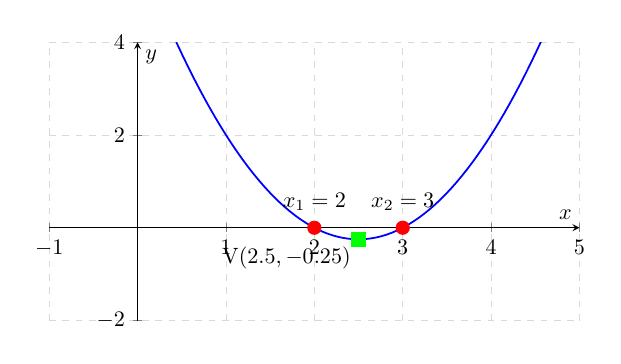
\begin{tikzpicture}[scale=0.8]
\begin{axis}[
    axis lines = center,
    xlabel = {$x$},
    ylabel = {$y$},
    ymin=-2, ymax=4,
    xmin=-1, xmax=5,
    grid=major,
    grid style={dashed,gray!30},
    width=10cm,
    height=6cm
]
% Parábola
\addplot[domain=-1:5, samples=100, thick, blue]{x^2-5*x+6};
% Raízes
\addplot[only marks, mark=*, mark size=3pt, red] coordinates {(2,0) (3,0)};
% Vértice
\addplot[only marks, mark=square*, mark size=3pt, green] coordinates {(2.5,-0.25)};
% Labels
\node[above] at (axis cs:2,0.2) {$x_1=2$};
\node[above] at (axis cs:3,0.2) {$x_2=3$};
\node[below left] at (axis cs:2.5,-0.25) {V$(2.5,-0.25)$};
\end{axis}
\end{tikzpicture}
\end{center}

\textbf{Interpretação geométrica final:}
As raízes $x_1 = 2$ e $x_2 = 3$ são os abcissas dos pontos de intersecção da parábola com o eixo dos xx. Geometricamente, representam os valores de $x$ para os quais a função $f(x) = x^2-5x+6$ se anula. A distância entre as raízes é $|x_2-x_1| = 1$, e o eixo de simetria da parábola passa pelo ponto médio entre elas, ou seja, em $x = 2.5$.
}
\FloatBarrier


\newpage

\section{3 - funcoes polinomiais grau nao superior 3}

% Exercise ID: MAT_P4FUNCOE_3FUN_001
% Module: MÓDULO P4 - Funções | Concept: Funções polinomiais de grau não superior a 3
% Difficulty: 2/5 (Fácil) | Type: desenvolvimento
% Author: Exemplo | Date: 2025-11-15
% Status: active

\exercicio{Considere a função $p(x)=x^3 - 2x^2 + 3x - 1$. Determine o seu grau e identifique os termos principais.
\vspace{3cm}
}

\FloatBarrier


\newpage

\section{4 - funcao inversa}

% Exercise ID: MAT_P4FUNCOE_4FIN_ANA_001
% meta:
% id: MAT_P4FUNCOE_4FIN_ANA_001
% title: "Determinação Analítica da Função Inversa"
% difficulty: 2
% tags: funcao_inversa, determinacao_analitica
% author: Generated Example
% has_subvariants: true

\section{Determinação Analítica da Função Inversa}

\exercicio{
Determina analiticamente a função inversa das seguintes expressões:
}

\begin{enumerate}[label=\alph*)]

\item % Sub-variant 1 for MAT_P4FUNCOE_4FIN_ANA_007
% Function: f(x) = x + 4

$f(x) = x + 4$

\item \input{subvariant_2}
\item % Sub-variant 3 for MAT_P4FUNCOE_4FIN_ANA_007
% Function: f(x) = \frac{1}{x-1}

$f(x) = \frac{2}{x-1}$

\item \input{subvariant_6}
\item \input{subvariant_6}
\item \input{subvariant_7}
\item % Exercise ID: MAT_P4FUNCOE_4FIN_ANA_001
% Sub-variant 8 for MAT_P4FUNCOE_4FIN_ANA_001
% Date: 2025-11-24
% Function: f(x) = \frac{1}{x-1}

$f(x) = \frac{6}{x-6}$
\item % Exercise ID: MAT_P4FUNCOE_4FIN_ANA_001
% Sub-variant 8 for MAT_P4FUNCOE_4FIN_ANA_001
% Date: 2025-11-24
% Function: f(x) = \frac{1}{x-1}

$f(x) = \frac{6}{x-6}$
\item % Exercise ID: MAT_P4FUNCOE_4FIN_ANA_001
% Sub-variant 9 for MAT_P4FUNCOE_4FIN_ANA_001
% Date: 2025-11-24
% Function: f(x) = \frac{1}{x-1}

$f(x) = \frac{7}{x-7}$
\item % Exercise ID: MAT_P4FUNCOE_4FIN_ANA_001
% Sub-variant 10 for MAT_P4FUNCOE_4FIN_ANA_001
% Date: 2025-11-24
% Function: f(x) = \frac{1}{x-1}

$f(x) = \frac{8}{x-8}$
\item \input{subvariant_11}
\end{enumerate}

\FloatBarrier

% Exercise ID: MAT_P4FUNCOE_4FX_DAX_001
% Module: MÓDULO P4 - Funções | Concept: Função Inversa | Type: Determinação Analítica da Função Inversa
% Difficulty: 2/5 (Fácil) | Format: standard
% Tags: inversa, expressao_analitica, algebra, calculo_analitico, injetividade, sobrejetividade, simetria, resolucao_equacao
% Author: Test Agent | Date: 2025-11-26
% Status: active

\exercicio{Determine a função inversa de f(x) = 2x + 3.}

\FloatBarrier

% Exercise ID: MAT_P4FUNCOE_4FX_DAX_002
% Module: MÓDULO P4 - Funções | Concept: Função Inversa | Type: Determinação Analítica da Função Inversa
% Difficulty: 2/5 (Fácil) | Format: standard
% Tags: algebra, simetria, resolucao_equacao, expressao_analitica, injetividade, inversa, sobrejetividade, calculo_analitico
% Author: Test Agent | Date: 2025-11-26
% Status: active

\exercicio{Determine a função inversa de f(x) = 2x + 3.}

\FloatBarrier

% meta:
% id: MAT_P4FUNCOE_4FX_DAX_003
% title: "MÓDULO P4 - Funções - Função Inversa - Determinação Analítica da Função Inversa"
% difficulty: 3
% tags: 
% author: Test Agent
% has_subvariants: true

\exercicio{
Determine analiticamente a função inversa das seguintes funções:
}

\begin{enumerate}[label=\alph*)]
\item {% Sub-variant 1 for MAT_P4FUNCOE_4FIN_ANA_007
% Function: f(x) = x + 4

$f(x) = x + 4$
}
\item {\input{subvariant_2.tex}}
\item {% Sub-variant 3 for MAT_P4FUNCOE_4FIN_ANA_007
% Function: f(x) = \frac{1}{x-1}

$f(x) = \frac{2}{x-1}$
}
\end{enumerate}


\FloatBarrier

% Exercise ID: MAT_P4FUNCOE_4FX_DAX_003
% Module: MÓDULO P4 - Funções | Concept: Função Inversa | Type: Determinação Analítica da Função Inversa
% Difficulty: 3/5 (Médio) | Format: standard
% Tags: resolucao_equacao, expressao_analitica, algebra, injetividade, simetria, sobrejetividade, calculo_analitico, inversa
% Author: Professor | Date: 2025-11-26
% Status: active

\exercicio{Teste de exercício}

\FloatBarrier

% Exercise ID: MAT_P4FUNCOE_4FX_DAX_004
% Created: 2025-11-26
% Difficulty: 2/5

\exercicio{Determine a função inversa de f(x) = 3x - 5.}

\FloatBarrier

% Exercise ID: MAT_P4FUNCOE_4FX_DAX_005
% Created: 2025-11-26
% Difficulty: 2/5

\exercicio{Determine a função inversa de f(x) = (x-1)/(x+1).}

\FloatBarrier

% Exercise ID: MAT_P4FUNCOE_4FX_DAX_006
% Module: MÓDULO P4 - Funções | Concept: Função Inversa | Type: Determinação Analítica da Função Inversa
% Difficulty: 2/5 (Fácil) | Format: standard
% Tags: inversa, resolucao_equacao, calculo_analitico, expressao_analitica, injetividade, algebra, sobrejetividade, simetria, funcao-inversa, equacao-linear, algebra
% Author: Professor | Date: 2025-11-27
% Status: active

\exercicio{Determine a função inversa de $f(x) = 2x + 3$. Apresente todos os passos de cálculo e verifique o resultado obtido.}

\FloatBarrier

% Solução do Exercício MAT_P4FUNCOE_4FX_DAX_006
% Determinação da função inversa de f(x) = 2x + 3

\exercicioDesenvolvimento{
\textbf{Solução Passo a Passo:}

\begin{enumerate}
\item \textbf{Verificar se a função é invertível:}
   \begin{itemize}
   \item A função $f(x) = 2x + 3$ é uma função linear com coeficiente $a = 2 \neq 0$.
   \item Como é uma função afim com coeficiente angular não nulo, ela é estritamente monótona (crescente).
   \item Portanto, $f(x)$ é bijetiva e possui função inversa.
   \end{itemize}

\item \textbf{Aplicar o método de troca de variáveis:}
   \begin{align}
   y &= 2x + 3 \\
   x &= 2y + 3 \quad \text{(troca $x \leftrightarrow y$)}
   \end{align}

\item \textbf{Isolar a nova variável $y$:}
   \begin{align}
   x &= 2y + 3 \\
   x - 3 &= 2y \\
   y &= \frac{x - 3}{2}
   \end{align}

\item \textbf{Escrever a função inversa:}
   \[f^{-1}(x) = \frac{x - 3}{2}\]

\item \textbf{Verificação do resultado:}
   \begin{itemize}
   \item Verificar $f(f^{-1}(x)) = x$:
     \[f\left(\frac{x - 3}{2}\right) = 2 \cdot \frac{x - 3}{2} + 3 = (x - 3) + 3 = x \checkmark\]
   
   \item Verificar $f^{-1}(f(x)) = x$:
     \[f^{-1}(2x + 3) = \frac{(2x + 3) - 3}{2} = \frac{2x}{2} = x \checkmark\]
   \end{itemize}

\item \textbf{Conclusão:}
   A função inversa de $f(x) = 2x + 3$ é:
   \[\boxed{f^{-1}(x) = \frac{x - 3}{2}}\]
\end{enumerate}

\textbf{Observações importantes:}
\begin{itemize}
\item O domínio de $f(x)$ é $\mathbb{R}$ e o contradomínio também é $\mathbb{R}$.
\item O domínio de $f^{-1}(x)$ é $\mathbb{R}$ (que era o contradomínio de $f$).
\item O contradomínio de $f^{-1}(x)$ é $\mathbb{R}$ (que era o domínio de $f$).
\item Graficamente, a função inversa é o reflexo de $f(x)$ em relação à reta $y = x$.
\end{itemize}
}
\FloatBarrier

% Exercise ID: MAT_P4FUNCOE_4FX_DAX_007
% Module: MÓDULO P4 - Funções | Concept: Função Inversa | Type: Determinação Analítica da Função Inversa
% Difficulty: 3/5 (Médio) | Format: standard
% Tags: resolucao_equacao, calculo_analitico, inversa, simetria, sobrejetividade, expressao_analitica, algebra, injetividade, inversa_racional
% Author: Professor | Date: 2025-11-27
% Status: active

\exercicio{Dada f(x)=\frac{3x-1}{2x+5}, determine analiticamente f^{-1}(x) e verifique f(f^{-1}(x))=x. Inclua justificações detalhadas para cada passo do processo.}

\exercicioDesenvolvimento{
\textbf{Passo 1: Verificar se a função é invertível}

Para que uma função tenha inversa, ela precisa ser bijetora (injetora e sobrejetora). 

A função f(x) = \frac{3x-1}{2x+5} é uma função racional com domínio D_f = \mathbb{R} \setminus \{-\frac{5}{2}\}.

Como é uma função racional com coeficientes diferentes nos termos de x no numerador e denominador, ela é estritamente monótona no seu domínio, portanto é injetora.

\textbf{Passo 2: Determinar a função inversa}

Para encontrar f^{-1}(x), resolvemos a equação y = \frac{3x-1}{2x+5} em ordem a x:

\begin{align}
y &= \frac{3x-1}{2x+5} \\
y(2x+5) &= 3x-1 \\
2xy + 5y &= 3x - 1 \\
2xy - 3x &= -1 - 5y \\
x(2y - 3) &= -1 - 5y \\
x &= \frac{-1 - 5y}{2y - 3}
\end{align}

Portanto, a função inversa é:
\[f^{-1}(x) = \frac{-1 - 5x}{2x - 3}\]

\textbf{Justificação:} Trocámos a variável y por x na expressão final, pois por convenção representamos a função inversa como f^{-1}(x).

\textbf{Passo 3: Verificar a composição f(f^{-1}(x)) = x}

Vamos verificar que f(f^{-1}(x)) = x:

\begin{align}
f(f^{-1}(x)) &= f\left(\frac{-1 - 5x}{2x - 3}\right) \\
&= \frac{3\left(\frac{-1 - 5x}{2x - 3}\right) - 1}{2\left(\frac{-1 - 5x}{2x - 3}\right) + 5} \\
&= \frac{\frac{3(-1 - 5x)}{2x - 3} - 1}{\frac{2(-1 - 5x)}{2x - 3} + 5} \\
&= \frac{\frac{-3 - 15x - (2x - 3)}{2x - 3}}{\frac{-2 - 10x + 5(2x - 3)}{2x - 3}} \\
&= \frac{\frac{-3 - 15x - 2x + 3}{2x - 3}}{\frac{-2 - 10x + 10x - 15}{2x - 3}} \\
&= \frac{\frac{-17x}{2x - 3}}{\frac{-17}{2x - 3}} \\
&= \frac{-17x}{2x - 3} \cdot \frac{2x - 3}{-17} \\
&= x
\end{align}

\textbf{Conclusão:} A verificação confirma que f^{-1}(x) = \frac{-1 - 5x}{2x - 3} é efetivamente a função inversa de f(x) = \frac{3x-1}{2x+5}, pois f(f^{-1}(x)) = x.

\textbf{Domínio e Contradomínio:}
- Domínio de f: D_f = \mathbb{R} \setminus \{-\frac{5}{2}\}
- Contradomínio de f: Im(f) = \mathbb{R} \setminus \{\frac{3}{2}\}
- Domínio de f^{-1}: D_{f^{-1}} = \mathbb{R} \setminus \{\frac{3}{2}\}
- Contradomínio de f^{-1}: Im(f^{-1}) = \mathbb{R} \setminus \{-\frac{5}{2}\}
}

\FloatBarrier

% Exercise ID: MAT_P4FUNCOE_4FX_DAX_018
% Created: 2025-11-27
% Difficulty: 2/5

\exercicio{Determine a função inversa de f(x) = 2x + 3. Apresente todos os passos de resolução e verifique se a função é bijetora.}

\exercicioDesenvolvimento{
\textbf{Passo 1: Verificar se a função é injetora}

Uma função é injetora (um-para-um) se valores diferentes de x produzem valores diferentes de f(x).

Para f(x) = 2x + 3:
\begin{itemize}
    \item É uma função linear com coeficiente angular a = 2 ≠ 0
    \item Funções lineares com coeficiente angular não nulo são estritamente monótonas
    \item Como a = 2 > 0, a função é estritamente crescente
    \item Portanto, f(x) é injetora
\end{itemize}

\textbf{Passo 2: Verificar se a função é sobrejetora}

Uma função é sobrejetora (sobre) se todo elemento do contradomínio tem pelo um antecedente no domínio.

Para f(x) = 2x + 3 com domínio D = ℝ e contradomínio CD = ℝ:
\begin{itemize}
    \item O limite quando x → -∞ é f(x) → -∞
    \item O limite quando x → +∞ é f(x) → +∞
    \item Pelo Teorema do Valor Intermediário, a função assume todos os valores reais
    \item Portanto, f(x) é sobrejetora
\end{itemize}

\textbf{Conclusão:} Como f(x) é injetora e sobrejetora, ela é \textbf{bijetora} e possui função inversa.

\textbf{Passo 3: Determinar a função inversa}

Para encontrar f⁻¹(x), seguimos o algoritmo:
\begin{enumerate}
    \item Trocar f(x) por y: y = 2x + 3
    \item Trocar x por y e y por x: x = 2y + 3
    \item Isolar y: x - 3 = 2y
    \item Resolver para y: y = \frac{x - 3}{2}
    \item Substituir y por f⁻¹(x): f⁻¹(x) = \frac{x - 3}{2}
\end{enumerate}

\textbf{Verificação:}
\begin{itemize}
    \item f(f⁻¹(x)) = 2 \cdot \frac{x - 3}{2} + 3 = x - 3 + 3 = x \quad \checkmark
    \item f⁻¹(f(x)) = \frac{2x + 3 - 3}{2} = \frac{2x}{2} = x \quad \checkmark
\end{itemize}

\textbf{Resposta final:} A função inversa é f⁻¹(x) = \frac{x - 3}{2}.
}

\FloatBarrier

% Exercise ID: MAT_P4FUNCOE_4FX_DAX_019
% Created: 2025-11-27
% Difficulty: 2/5

\exercicio{Determine a função inversa de f(x) = 2x + 3. Apresente todos os passos de cálculo, incluindo a verificação da condição de injetividade e a comprovação do resultado através da composição de funções.}

\FloatBarrier

% Solução do Exercício MAT_P4FUNCOE_4FX_DAX_019
% Determinação da função inversa de f(x) = 2x + 3

\exercicioDesenvolvimento{
\textbf{Solução Passo a Passo:}

\begin{enumerate}
\item \textbf{Verificar se a função é invertível (injetiva):}
   \begin{itemize}
   \item A função $f(x) = 2x + 3$ é uma função afim com coeficiente angular $a = 2 \neq 0$.
   \item Como $a > 0$, a função é estritamente crescente em todo o seu domínio.
   \item Uma função estritamente monótona é necessariamente injetiva.
   \item Portanto, $f(x)$ é bijetora em $\mathbb{R}$ e possui função inversa.
   \end{itemize}

\item \textbf{Aplicar o método de troca de variáveis:}
   \begin{align}
   y &= 2x + 3 \\
   x &= 2y + 3 \quad \text{(troca $x \leftrightarrow y$)}
   \end{align}

\item \textbf{Isolar a nova variável $y$:}
   \begin{align}
   x &= 2y + 3 \\
   x - 3 &= 2y \\
   y &= \frac{x - 3}{2}
   \end{align}

\item \textbf{Escrever a função inversa:}
   \[f^{-1}(x) = \frac{x - 3}{2}\]

\item \textbf{Verificação através da composição de funções:}
   \begin{itemize}
   \item Verificar $f(f^{-1}(x)) = x$:
     \begin{align}
     f\left(\frac{x - 3}{2}\right) &= 2 \cdot \frac{x - 3}{2} + 3 \\
     &= (x - 3) + 3 \\
     &= x \checkmark
     \end{align}
   
   \item Verificar $f^{-1}(f(x)) = x$:
     \begin{align}
     f^{-1}(2x + 3) &= \frac{(2x + 3) - 3}{2} \\
     &= \frac{2x}{2} \\
     &= x \checkmark
     \end{align}
   \end{itemize}

\item \textbf{Análise dos domínios e contradomínios:}
   \begin{itemize}
   \item Domínio de $f$: $\mathcal{D}_f = \mathbb{R}$
   \item Contradomínio de $f$: $\mathcal{C}_f = \mathbb{R}$
   \item Domínio de $f^{-1}$: $\mathcal{D}_{f^{-1}} = \mathbb{R}$ (igual ao contradomínio de $f$)
   \item Contradomínio de $f^{-1}$: $\mathcal{C}_{f^{-1}} = \mathbb{R}$ (igual ao domínio de $f$)
   \end{itemize}
\end{enumerate}

\textbf{Conclusão:}
A função inversa de $f(x) = 2x + 3$ é:
\[\boxed{f^{-1}(x) = \frac{x - 3}{2}}\]

\textbf{Observações importantes:}
\begin{itemize}
\item Graficamente, a função inversa é o reflexo de $f(x)$ em relação à reta $y = x$.
\item A composição $f \circ f^{-1} = f^{-1} \circ f = \text{id}_{\mathbb{R}}$ confirma a corretude do resultado.
\item O ponto $(0, 3)$ em $f(x)$ corresponde ao ponto $(3, 0)$ em $f^{-1}(x)$.
\end{itemize}
}
\FloatBarrier

% Exercise ID: MAT_P4FUNCOE_4FX_DAX_021
% Created: 2025-11-27
% Difficulty: 2/5

\exercicio{Dada a função $f(x) = 2x + 3$, determine a função inversa $f^{-1}(x)$ e justifique todos os passos do seu raciocínio.}

\FloatBarrier

% Exercise ID: MAT_P4FUNCOE_4FX_DAX_022
% Created: 2025-11-27
% Difficulty: 2/5

\exercicio{Dada f(x)=2x+3 determine f^{-1} e justifique}

\FloatBarrier

% Exercise ID: MAT_P4FUNCOE_4FX_DAX_023
% Created: 2025-11-27
% Difficulty: 2/5

\exercicio{Determine a função inversa de $f(x) = 2x + 3$. Apresente todos os passos algébricos necessários e verifique se a função é bijetora.}

\FloatBarrier

% Exercise ID: MAT_P4FUNCOE_4FX_DAX_023
% Solution File
% Created: 2025-11-27
% Difficulty: 2/5

\exercicioDesenvolvimento{Solução: Determinação da função inversa de $f(x) = 2x + 3$}

\textbf{Passo 1: Verificar se a função é injetora}

Uma função é injetora (um-para-um) se $f(a) = f(b) \Rightarrow a = b$.

Seja $f(a) = f(b)$:
$$2a + 3 = 2b + 3$$
$$2a = 2b$$
$$a = b$$

Portanto, $f$ é injetora.

\textbf{Passo 2: Verificar se a função é sobrejetora}

Uma função é sobrejetora (sobre) se para todo $y \in \mathbb{R}$, existe $x \in \mathbb{R}$ tal que $f(x) = y$.

Seja $y \in \mathbb{R}$ qualquer. Queremos encontrar $x$ tal que:
$$2x + 3 = y$$
$$2x = y - 3$$
$$x = \frac{y - 3}{2}$$

Como $\frac{y - 3}{2} \in \mathbb{R}$ para qualquer $y \in \mathbb{R}$, a função é sobrejetora.

\textbf{Conclusão:} Como $f$ é injetora e sobrejetora, ela é \textbf{bijetora} e possui função inversa.

\textbf{Passo 3: Determinar a função inversa}

Para encontrar $f^{-1}(x)$, seguimos o algoritmo padrão:

\begin{enumerate}
    \item Trocar $f(x)$ por $y$:
    $$y = 2x + 3$$
    
    \item Trocar $x$ por $y$ e $y$ por $x$:
    $$x = 2y + 3$$
    
    \item Isolar $y$:
    $$x - 3 = 2y$$
    $$y = \frac{x - 3}{2}$$
    
    \item Substituir $y$ por $f^{-1}(x)$:
    $$f^{-1}(x) = \frac{x - 3}{2}$$
\end{enumerate}

\textbf{Passo 4: Verificação}

Vamos verificar que $f(f^{-1}(x)) = x$ e $f^{-1}(f(x)) = x$:

$$f(f^{-1}(x)) = f\left(\frac{x - 3}{2}\right) = 2 \cdot \frac{x - 3}{2} + 3 = x - 3 + 3 = x \checkmark$$

$$f^{-1}(f(x)) = f^{-1}(2x + 3) = \frac{(2x + 3) - 3}{2} = \frac{2x}{2} = x \checkmark$$

\textbf{Resposta Final:} A função inversa de $f(x) = 2x + 3$ é:
$$\boxed{f^{-1}(x) = \frac{x - 3}{2}}$$
\FloatBarrier

% Exercise ID: MAT_P4FUNCOE_4FX_DAX_025
% Created: 2025-11-27
% Difficulty: 2/5

\exercicio{Determine a função inversa de f(x) = 2x + 3. Apresente todos os passos de resolução, incluindo verificação da bijetividade e composição das funções.}

\exercicioDesenvolvimento{
\textbf{Passo 1: Verificar se a função é bijetora}

Para que uma função possua inversa, ela precisa ser bijetora (injetora e sobrejetora).

\textbf{Injetividade:}
Uma função é injetora se f(x₁) = f(x₂) ⇒ x₁ = x₂.

Para f(x) = 2x + 3:
\begin{align*}
f(x_1) &= f(x_2) \\
2x_1 + 3 &= 2x_2 + 3 \\
2x_1 &= 2x_2 \\
x_1 &= x_2
\end{align*}

Portanto, f(x) é injetora.

\textbf{Sobrejetividade:}
Como f(x) = 2x + 3 é uma função linear com coeficiente angular não nulo, seu contradomínio natural é ℝ. Para qualquer y ∈ ℝ, existe x = (y-3)/2 ∈ ℝ tal que f(x) = y. Portanto, f(x) é sobrejetora.

\textbf{Conclusão:} f(x) é bijetora e possui função inversa.

\textbf{Passo 2: Determinar a função inversa}

Aplicamos o algoritmo para encontrar f⁻¹(x):

\begin{enumerate}
    \item Escrevemos y = f(x): \quad y = 2x + 3
    \item Trocamos x por y: \quad x = 2y + 3
    \item Isolamos y: \quad x - 3 = 2y
    \item Resolvemos para y: \quad y = \frac{x - 3}{2}
    \item Substituímos y por f⁻¹(x): \quad f^{-1}(x) = \frac{x - 3}{2}
\end{enumerate}

\textbf{Passo 3: Verificação por composição}

Verificamos se f(f⁻¹(x)) = x e f⁻¹(f(x)) = x:

\begin{align*}
f(f^{-1}(x)) &= 2 \cdot \left(\frac{x - 3}{2}\right) + 3 \\
&= (x - 3) + 3 \\
&= x \quad \checkmark
\end{align*}

\begin{align*}
f^{-1}(f(x)) &= \frac{2x + 3 - 3}{2} \\
&= \frac{2x}{2} \\
&= x \quad \checkmark
\end{align*}

\textbf{Resposta final:} A função inversa é $f^{-1}(x) = \frac{x - 3}{2}$.
}

\FloatBarrier

% Exercise ID: MAT_P4FUNCOE_FUNC_DA_001
% Module: P4_funcoes | Concept: 4-funcao_inversa
% Type: determinacao_analitica | Difficulty: 2/5
% Tags: funcao_inversa, determinacao analitica, funcoes, inversa
% Author: Professor | Date: 2025-11-26

\exercicio{
Determine a função inversa de $f(x) = 2x + 3$.
}

\subexercicio{Verifique que $f(f^{-1}(x))=x$ para todo $x$ no domínio.}
\FloatBarrier

% Exercise ID: MAT_P4FUNCOE_FUNC_DA_001
% Module: P4_funcoes | Concept: 4-funcao_inversa
% Type: determinacao_analitica | Difficulty: 2/5
% Tags: funcao_inversa, determinacao analitica, funcoes, inversa
% Author: Professor | Date: 2025-11-26

\exercicio{
Determine a função inversa de $f(x) = 2x + 3$.
}

\subexercicio{Verifique que $f(f^{-1}(x))=x$ para todo $x$ no domínio.}


\FloatBarrier

% Exercise ID: MAT_P4FUNCOE_FUNC_DA_001
% Module: P4_funcoes | Concept: 4-funcao_inversa
% Type: determinacao_analitica | Difficulty: 2/5
% Tags: funcao_inversa, determinacao analitica, funcoes, inversa
% Author: Professor | Date: 2025-11-26

\exercicio{
Determine a função inversa de $f(x) = 2x + 3$.
}

\subexercicio{Verifique que $f(f^{-1}(x))=x$ para todo $x$ no domínio.}

\FloatBarrier

% Exercise ID: MAT_P4FUNCOE_FUNC_DA_002
% Module: P4_funcoes | Concept: 4-funcao_inversa
% Type: determinacao_analitica | Difficulty: 2/5
% Tags: funcao_inversa, determinacao analitica, funcoes, inversa
% Author: Professor | Date: 2025-11-26

\exercicio{
Determine a função inversa de $f(x) = 2x + 3$.
}

\subexercicio{Verifique que $f(f^{-1}(x))=x$ para todo $x$ no domínio.}
\FloatBarrier

% Exercise ID: MAT_P4FUNCOE_FUNC_DA_002
% Module: P4_funcoes | Concept: 4-funcao_inversa
% Type: determinacao_analitica | Difficulty: 2/5
% Tags: funcao_inversa, determinacao analitica, funcoes, inversa
% Author: Professor | Date: 2025-11-26

\exercicio{
Determine a função inversa de $f(x) = 2x + 3$.
}

\subexercicio{Verifique que $f(f^{-1}(x))=x$ para todo $x$ no domínio.}


\FloatBarrier

% Exercise ID: MAT_P4FUNCOE_FUNC_DA_002
% Module: P4_funcoes | Concept: 4-funcao_inversa
% Type: determinacao_analitica | Difficulty: 2/5
% Tags: funcao_inversa, determinacao analitica, funcoes, inversa
% Author: Professor | Date: 2025-11-26

\exercicio{
Determine a função inversa de $f(x) = 2x + 3$.
}

\subexercicio{Verifique que $f(f^{-1}(x))=x$ para todo $x$ no domínio.}

\FloatBarrier

% Exercise ID: MAT_P4FUNCOE_FUNC_DA_003
% Module: P4_funcoes | Concept: 4-funcao_inversa
% Type: determinacao_analitica | Difficulty: 2/5
% Tags: funcao_inversa, determinacao analitica, funcoes, inversa
% Author: Professor | Date: 2025-11-26

\exercicio{
Determine a função inversa de $f(x) = 2x + 3$.
}

\subexercicio{Verifique que $f(f^{-1}(x))=x$ para todo $x$ no domínio.}
\FloatBarrier

% Exercise ID: MAT_P4FUNCOE_FUNC_DA_003
% Module: P4_funcoes | Concept: 4-funcao_inversa
% Type: determinacao_analitica | Difficulty: 2/5
% Tags: funcao_inversa, determinacao analitica, funcoes, inversa
% Author: Professor | Date: 2025-11-26

\exercicio{
Determine a função inversa de $f(x) = 2x + 3$.
}

\subexercicio{Verifique que $f(f^{-1}(x))=x$ para todo $x$ no domínio.}


\FloatBarrier

% Exercise ID: MAT_P4FUNCOE_FUNC_DA_003
% Module: P4_funcoes | Concept: 4-funcao_inversa
% Type: determinacao_analitica | Difficulty: 2/5
% Tags: funcao_inversa, determinacao analitica, funcoes, inversa
% Author: Professor | Date: 2025-11-26

\exercicio{
Determine a função inversa de $f(x) = 2x + 3$.
}

\subexercicio{Verifique que $f(f^{-1}(x))=x$ para todo $x$ no domínio.}

\FloatBarrier

% Exercise ID: MAT_P4FUNCOE_4FIN_ANA_001
% Module: MÓDULO P4 - Funções | Concept: Função Inversa | Type: Determinação Analítica
% Difficulty: 2/5 (Fácil) | Type: desenvolvimento
% Points: 10 | Time: 10 min
% Tags: inversa, funcao_linear, grafico, expressao_analitica
% Author: Professor | Date: 2025-11-18
% Status: active
% Description: Determinar expressão analítica e representar graficamente função e inversa

\exercicio{
Considere a função $f(x) = 2x - 3$.

\begin{enumerate}[label=\alph*]
    \item Determine a expressão analítica da função inversa $f^{-1}(x)$.
    
    \vspace{3cm}
    \item Represente graficamente a função $f$ e a sua inversa $f^{-1}$ no mesmo referencial.
    
    \vspace{3cm}

    \begin{center}
    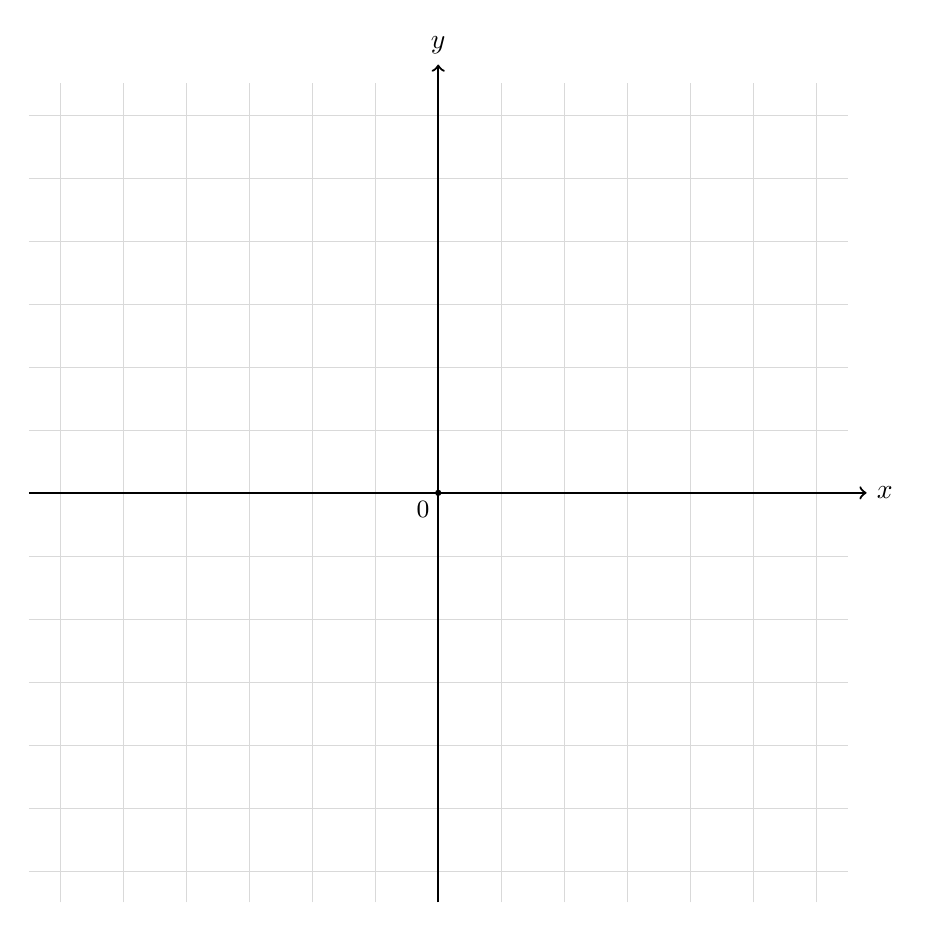
\begin{tikzpicture}[scale=0.8]
        % grid
        \draw[step=1cm,gray!30,very thin] (-6.5,-6.5) grid (6.5,6.5);
        % axes
        \draw[->,thick] (-6.5,0) -- (6.8,0) node[right] {$x$};
        \draw[->,thick] (0,-6.5) -- (0,6.8) node[above] {$y$};
        % origin
        \fill (0,0) circle (0.05) node[below left=2pt,fill=white,inner sep=1pt] {\small $0$};
    \end{tikzpicture}
    \end{center}
\end{enumerate}
}
\FloatBarrier

% Exercise ID: MAT_P4FUNCOE_4FIN_ANA_001
% Module: MÓDULO P4 - Funções | Concept: Função Inversa | Type: Determinação Analítica
% Difficulty: 2/5 (Fácil) | Type: desenvolvimento
% Points: 10 | Time: 10 min
% Tags: inversa, funcao_linear, grafico, expressao_analitica
% Author: Professor | Date: 2025-11-18
% Status: active
% Description: Determinar expressão analítica e representar graficamente função e inversa

\exercicio
Considere a função $f(x) = 2x - 3$.

\begin{enumerate}[label=\alph*]
    \item Determine a expressão analítica da função inversa $f^{-1}(x)$.
    
    \vspace{3cm}
    \item Represente graficamente a função $f$ e a sua inversa $f^{-1}$ no mesmo referencial.
    
    \vspace{3cm}

    \begin{center}
    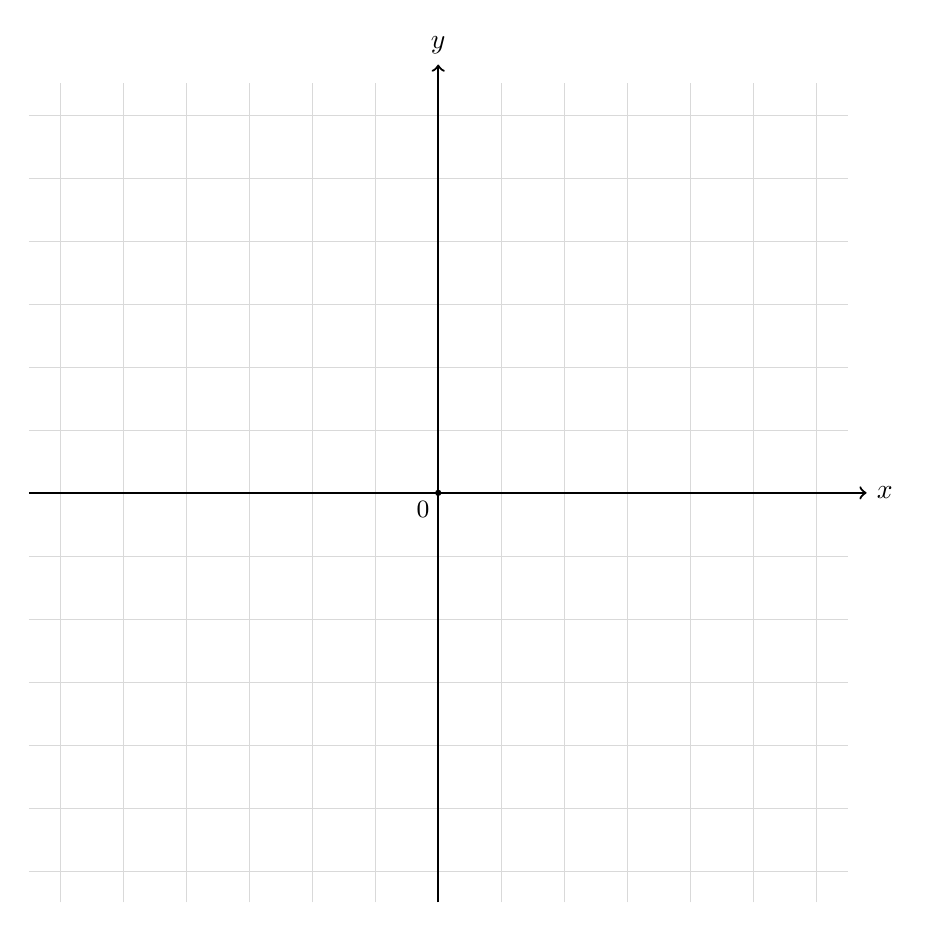
\begin{tikzpicture}[scale=0.8]
        % grid
        \draw[step=1cm,gray!30,very thin] (-6.5,-6.5) grid (6.5,6.5);
        % axes
        \draw[->,thick] (-6.5,0) -- (6.8,0) node[right] {$x$};
        \draw[->,thick] (0,-6.5) -- (0,6.8) node[above] {$y$};
        % origin
        \fill (0,0) circle (0.05) node[below left=2pt,fill=white,inner sep=1pt] {\small $0$};
    \end{tikzpicture}
    \end{center}
\end{enumerate}
\FloatBarrier

% Exercise ID: MAT_P4FUNCOE_4FIN_ANA_001
% Module: MÓDULO P4 - Funções | Concept: Função Inversa | Type: Determinação Analítica
% Difficulty: 2/5 (Fácil) | Type: desenvolvimento
% Points: 10 | Time: 10 min
% Tags: inversa, funcao_linear, grafico, expressao_analitica
% Author: Professor | Date: 2025-11-18
% Status: active
% Description: Determinar expressão analítica e representar graficamente função e inversa

\exercicio{
Considere a função $f(x) = 2x - 3$.

\begin{enumerate}[label=\alph*]
    \item Determine a expressão analítica da função inversa $f^{-1}(x)$.
    
    \vspace{3cm}
    \item Represente graficamente a função $f$ e a sua inversa $f^{-1}$ no mesmo referencial.
    
    \vspace{3cm}

    \begin{center}
    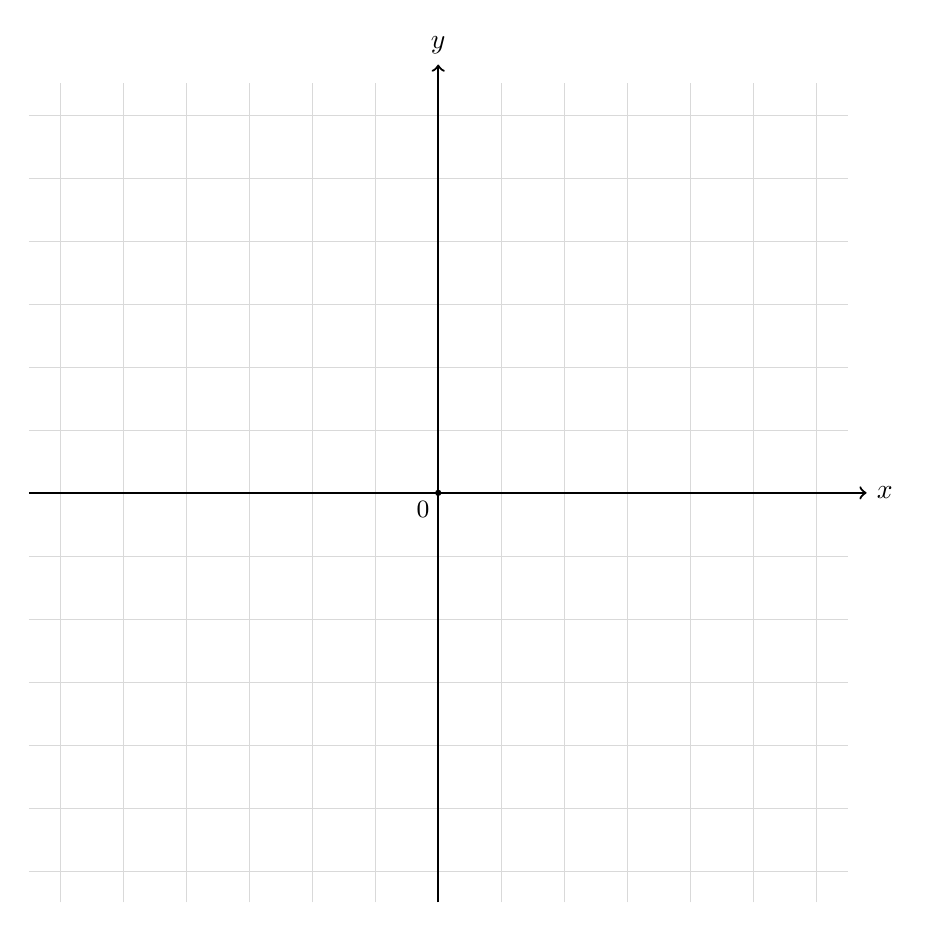
\begin{tikzpicture}[scale=0.8]
        % grid
        \draw[step=1cm,gray!30,very thin] (-6.5,-6.5) grid (6.5,6.5);
        % axes
        \draw[->,thick] (-6.5,0) -- (6.8,0) node[right] {$x$};
        \draw[->,thick] (0,-6.5) -- (0,6.8) node[above] {$y$};
        % origin
        \fill (0,0) circle (0.05) node[below left=2pt,fill=white,inner sep=1pt] {\small $0$};
    \end{tikzpicture}
    \end{center}
\end{enumerate}
}
\FloatBarrier

% Exercise ID: MAT_P4FUNCOE_4FIN_ANA_002
% Module: MÓDULO P4 - Funções | Concept: Função Inversa | Type: Determinação Analítica
% Difficulty: 2/5 (Fácil) | Type: desenvolvimento
% Points: 10 | Time: 10 min
% Tags: inversa, expressao_analitica, calculo
% Author: Professor | Date: 2025-11-18
% Status: active
% Description: Calcular a expressão da inversa de funções simples

\exercicio
Considere a função $f(x) = x - 1$.

\begin{enumerate}[label=\alph*]
    \item Determine a expressão analítica da função inversa $f^{-1}(x)$.
    
    \vspace{3cm}
    \item Represente graficamente a função $f$ e a sua inversa $f^{-1}$ no mesmo referencial.

        \begin{center}
    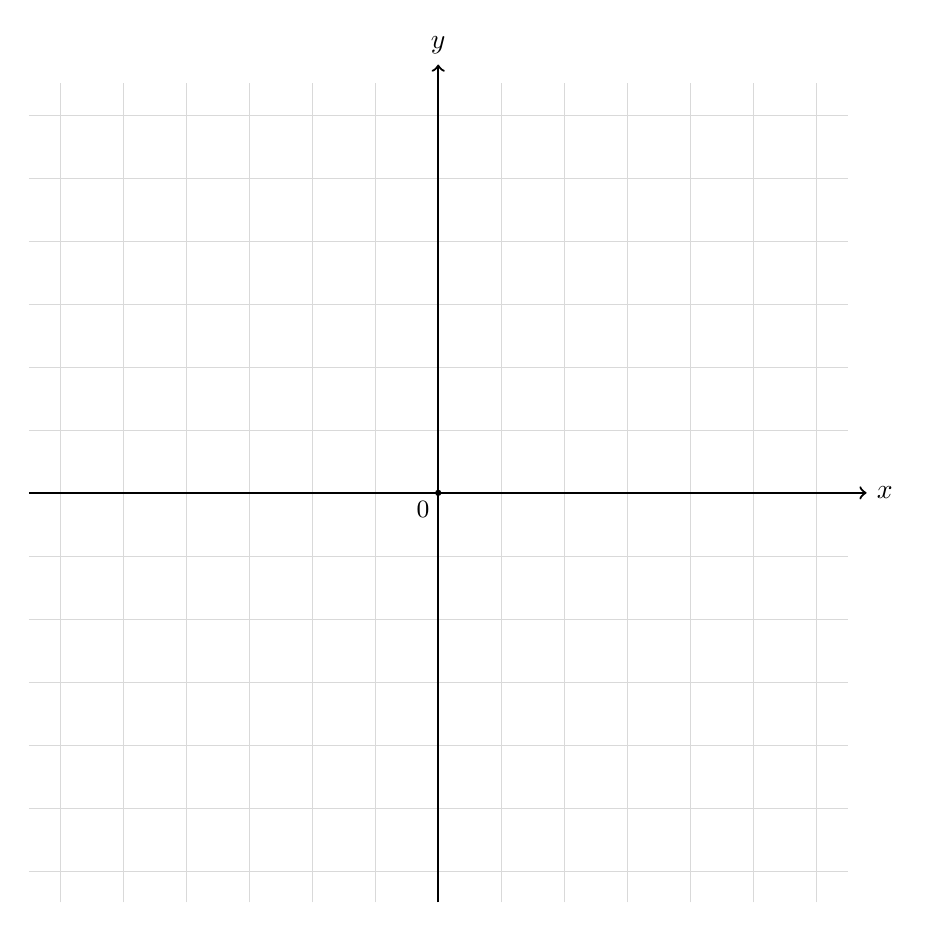
\begin{tikzpicture}[scale=0.8]
        % grid
        \draw[step=1cm,gray!30,very thin] (-6.5,-6.5) grid (6.5,6.5);
        % axes
        \draw[->,thick] (-6.5,0) -- (6.8,0) node[right] {$x$};
        \draw[->,thick] (0,-6.5) -- (0,6.8) node[above] {$y$};
        % origin
        \fill (0,0) circle (0.05) node[below left=2pt,fill=white,inner sep=1pt] {\small $0$};
    \end{tikzpicture}
    \end{center}

\end{enumerate}
\FloatBarrier

% Exercise ID: MAT_P4FUNCOE_4FIN_ANA_002
% Module: MÓDULO P4 - Funções | Concept: Função Inversa | Type: Determinação Analítica
% Difficulty: 2/5 (Fácil) | Type: desenvolvimento
% Points: 10 | Time: 10 min
% Tags: inversa, expressao_analitica, calculo
% Author: Professor | Date: 2025-11-18
% Status: active
% Description: Calcular a expressão da inversa de funções simples

\exercicio
Considere a função $f(x) = x - 1$.

\begin{enumerate}[label=\alph*]
    \item Determine a expressão analítica da função inversa $f^{-1}(x)$.
    
    \vspace{3cm}
    \item Represente graficamente a função $f$ e a sua inversa $f^{-1}$ no mesmo referencial.

        \begin{center}
    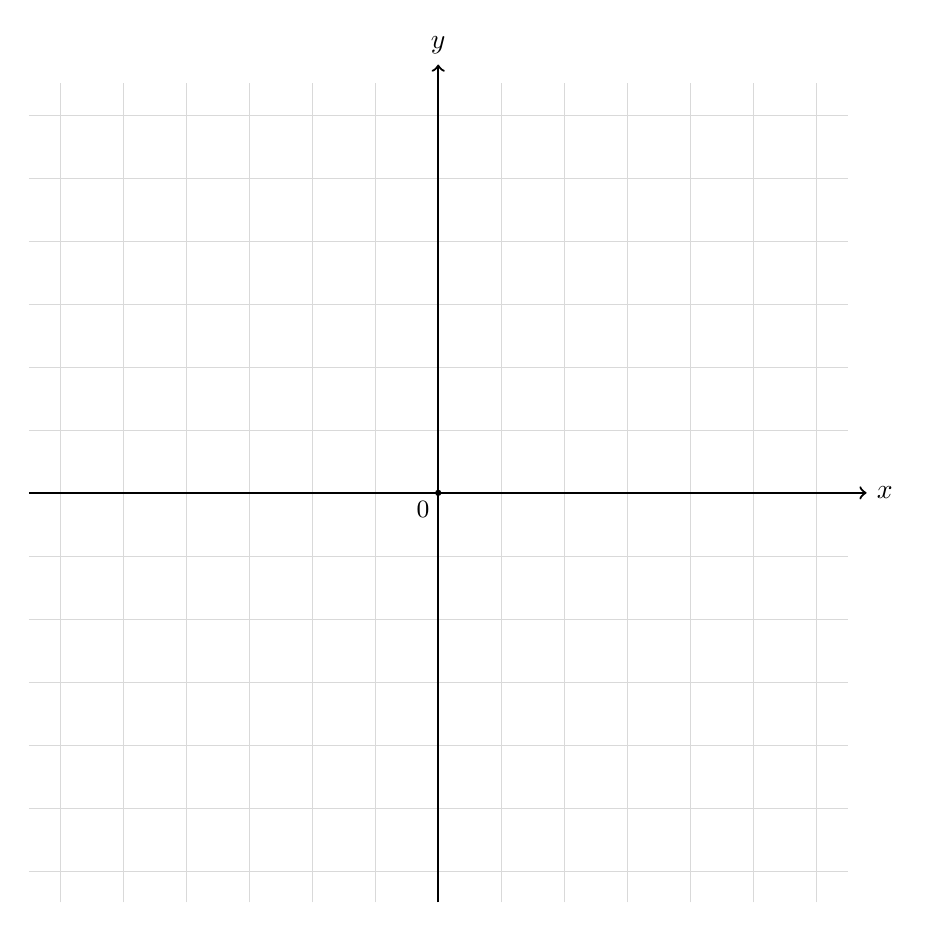
\begin{tikzpicture}[scale=0.8]
        % grid
        \draw[step=1cm,gray!30,very thin] (-6.5,-6.5) grid (6.5,6.5);
        % axes
        \draw[->,thick] (-6.5,0) -- (6.8,0) node[right] {$x$};
        \draw[->,thick] (0,-6.5) -- (0,6.8) node[above] {$y$};
        % origin
        \fill (0,0) circle (0.05) node[below left=2pt,fill=white,inner sep=1pt] {\small $0$};
    \end{tikzpicture}
    \end{center}

\end{enumerate}
\FloatBarrier

% Exercise ID: MAT_P4FUNCOE_4FIN_ANA_002
% Module: MÓDULO P4 - Funções | Concept: Função Inversa | Type: Determinação Analítica
% Difficulty: 2/5 (Fácil) | Type: desenvolvimento
% Points: 10 | Time: 10 min
% Tags: inversa, expressao_analitica, calculo
% Author: Professor | Date: 2025-11-18
% Status: active
% Description: Calcular a expressão da inversa de funções simples

\exercicio
Considere a função $f(x) = x - 1$.

\begin{enumerate}[label=\alph*]
    \item Determine a expressão analítica da função inversa $f^{-1}(x)$.
    
    \vspace{3cm}
    \item Represente graficamente a função $f$ e a sua inversa $f^{-1}$ no mesmo referencial.

        \begin{center}
    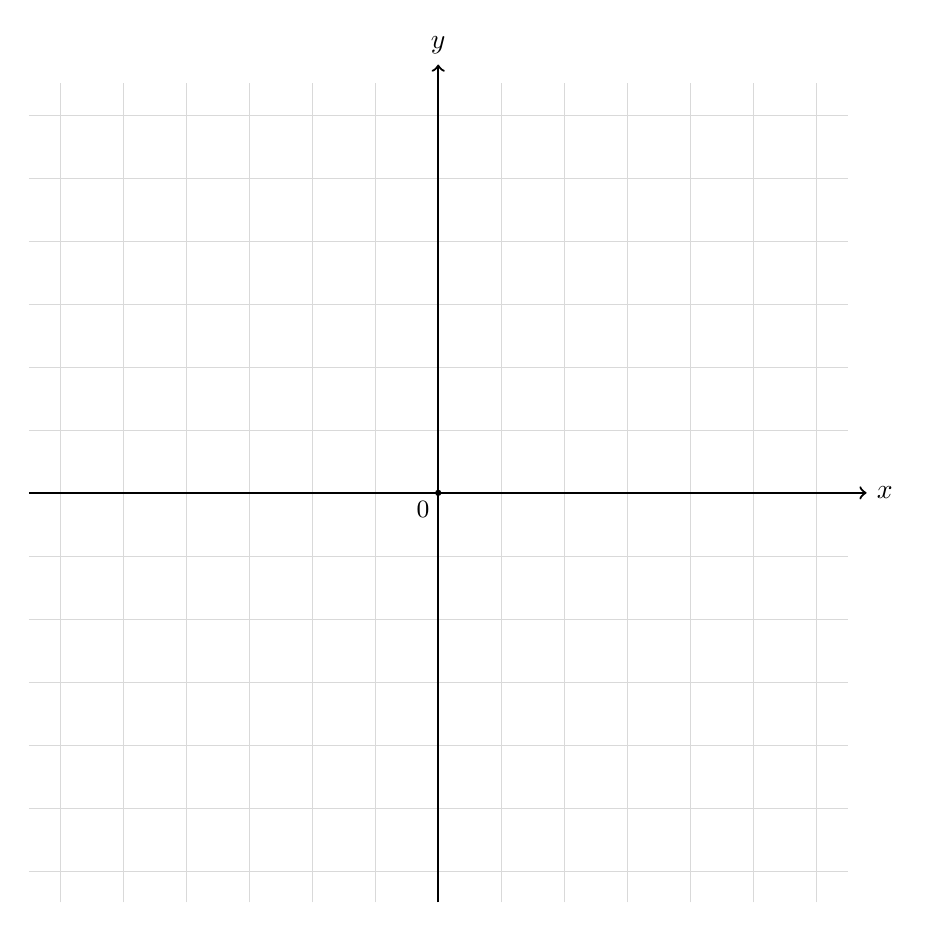
\begin{tikzpicture}[scale=0.8]
        % grid
        \draw[step=1cm,gray!30,very thin] (-6.5,-6.5) grid (6.5,6.5);
        % axes
        \draw[->,thick] (-6.5,0) -- (6.8,0) node[right] {$x$};
        \draw[->,thick] (0,-6.5) -- (0,6.8) node[above] {$y$};
        % origin
        \fill (0,0) circle (0.05) node[below left=2pt,fill=white,inner sep=1pt] {\small $0$};
    \end{tikzpicture}
    \end{center}

\end{enumerate}
\FloatBarrier

% Exercise ID: MAT_P4FUNCOE_4FIN_005
% Exercise ID: MAT_P4FUNCOE_4FIN_ANA_003
% Module: MÓDULO P4 - Funções | Concept: Função Inversa | Type: Determinação Analítica
% Difficulty: 2/5 (Fácil) | Type: desenvolvimento
% Points: 10 | Time: 10 min
% Tags: inversa, funcao_linear, grafico, expressao_analitica
% Author: Professor | Date: 2025-11-18
% Status: active
% Description: Determinar expressão analítica e representar graficamente função e inversa

\exercicio
Considere a função $f(x) = 2x - 4$.

\begin{enumerate}[label=\alph*]
    \item Determine a expressão analítica da função inversa $f^{-1}(x)$.
    
    \vspace{3cm}
    \item Represente graficamente a função $f$ e a sua inversa $f^{-1}$ no mesmo referencial.

        \begin{center}
    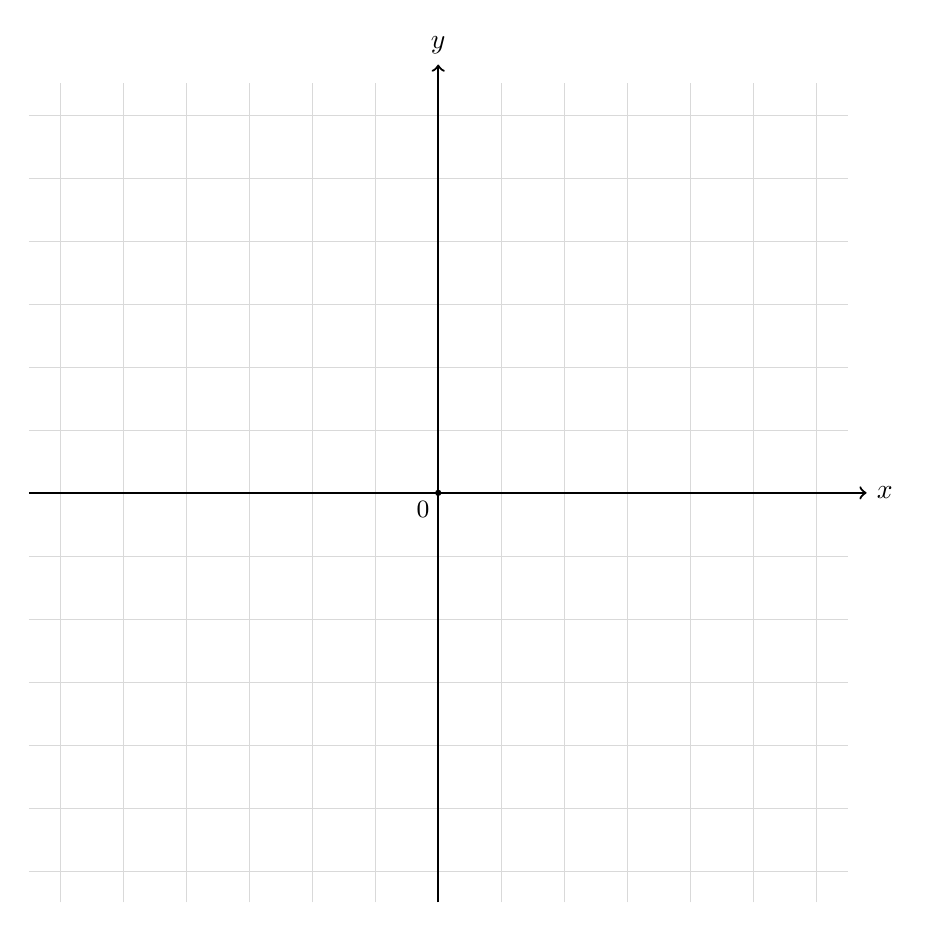
\begin{tikzpicture}[scale=0.8]
        % grid
        \draw[step=1cm,gray!30,very thin] (-6.5,-6.5) grid (6.5,6.5);
        % axes
        \draw[->,thick] (-6.5,0) -- (6.8,0) node[right] {$x$};
        \draw[->,thick] (0,-6.5) -- (0,6.8) node[above] {$y$};
        % origin
        \fill (0,0) circle (0.05) node[below left=2pt,fill=white,inner sep=1pt] {\small $0$};
    \end{tikzpicture}
    \end{center}

\end{enumerate}
\FloatBarrier

% Exercise ID: MAT_P4FUNCOE_4FIN_005
% Exercise ID: MAT_P4FUNCOE_4FIN_ANA_003
% Module: MÓDULO P4 - Funções | Concept: Função Inversa | Type: Determinação Analítica
% Difficulty: 2/5 (Fácil) | Type: desenvolvimento
% Points: 10 | Time: 10 min
% Tags: inversa, funcao_linear, grafico, expressao_analitica
% Author: Professor | Date: 2025-11-18
% Status: active
% Description: Determinar expressão analítica e representar graficamente função e inversa

\exercicio
Considere a função $f(x) = 2x - 4$.

\begin{enumerate}[label=\alph*]
    \item Determine a expressão analítica da função inversa $f^{-1}(x)$.
    
    \vspace{3cm}
    \item Represente graficamente a função $f$ e a sua inversa $f^{-1}$ no mesmo referencial.

        \begin{center}
    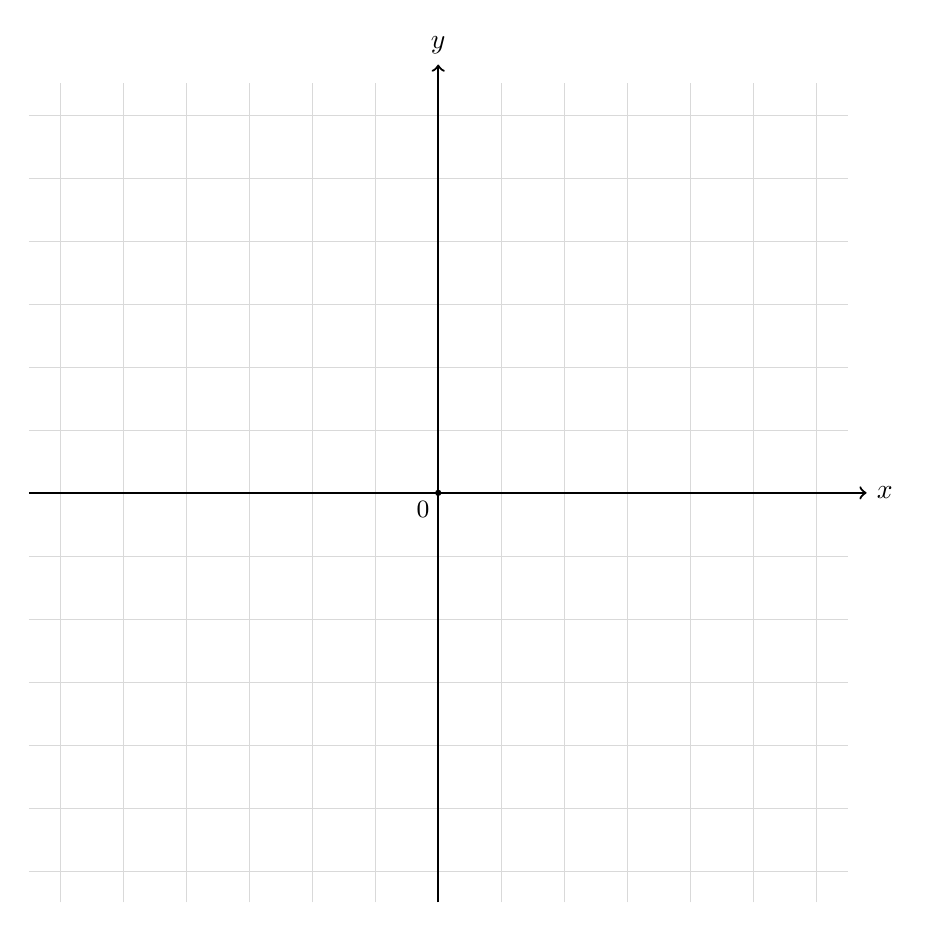
\begin{tikzpicture}[scale=0.8]
        % grid
        \draw[step=1cm,gray!30,very thin] (-6.5,-6.5) grid (6.5,6.5);
        % axes
        \draw[->,thick] (-6.5,0) -- (6.8,0) node[right] {$x$};
        \draw[->,thick] (0,-6.5) -- (0,6.8) node[above] {$y$};
        % origin
        \fill (0,0) circle (0.05) node[below left=2pt,fill=white,inner sep=1pt] {\small $0$};
    \end{tikzpicture}
    \end{center}

\end{enumerate}
\FloatBarrier

% Exercise ID: MAT_P4FUNCOE_4FIN_005
% Exercise ID: MAT_P4FUNCOE_4FIN_ANA_003
% Module: MÓDULO P4 - Funções | Concept: Função Inversa | Type: Determinação Analítica
% Difficulty: 2/5 (Fácil) | Type: desenvolvimento
% Points: 10 | Time: 10 min
% Tags: inversa, funcao_linear, grafico, expressao_analitica
% Author: Professor | Date: 2025-11-18
% Status: active
% Description: Determinar expressão analítica e representar graficamente função e inversa

\exercicio
Considere a função $f(x) = 2x - 4$.

\begin{enumerate}[label=\alph*]
    \item Determine a expressão analítica da função inversa $f^{-1}(x)$.
    
    \vspace{3cm}
    \item Represente graficamente a função $f$ e a sua inversa $f^{-1}$ no mesmo referencial.

        \begin{center}
    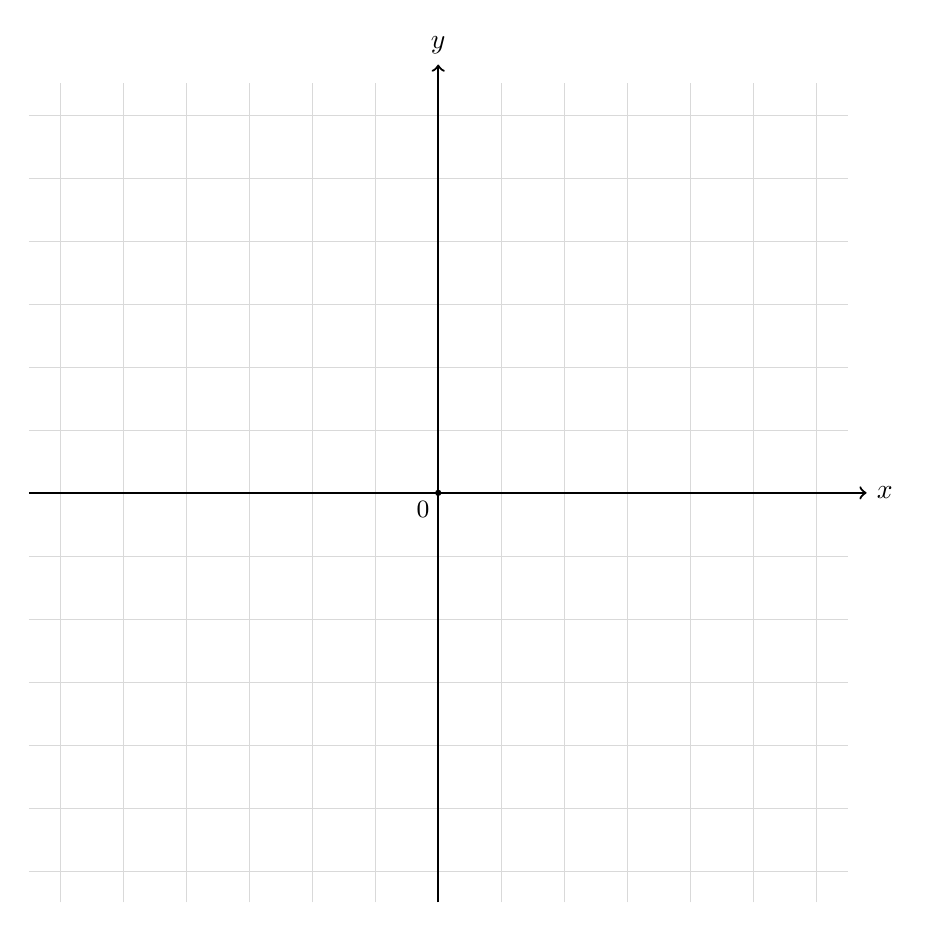
\begin{tikzpicture}[scale=0.8]
        % grid
        \draw[step=1cm,gray!30,very thin] (-6.5,-6.5) grid (6.5,6.5);
        % axes
        \draw[->,thick] (-6.5,0) -- (6.8,0) node[right] {$x$};
        \draw[->,thick] (0,-6.5) -- (0,6.8) node[above] {$y$};
        % origin
        \fill (0,0) circle (0.05) node[below left=2pt,fill=white,inner sep=1pt] {\small $0$};
    \end{tikzpicture}
    \end{center}

\end{enumerate}
\FloatBarrier

% Exercise ID: MAT_P4FUNCOE_4FIN_ANA_004
% Exercise ID: MAT_P4FUNCOE_4FIN_ANA_004
% Module: MÓDULO P4 - Funções | Concept: Função Inversa | Type: Determinação Analítica
% Difficulty: 2/5 (Fácil) | Type: desenvolvimento
% Points: 10 | Time: 10 min
% Tags: inversa, funcao_linear, grafico, expressao_analitica
% Author: Professor | Date: 2025-11-18
% Status: active
% Description: Determinar expressão analítica e representar graficamente função e inversa

\exercicio
Considere a função $f(x) = 3x - 1$.

\begin{enumerate}[label=\alph*]
    \item Determine a expressão analítica da função inversa $f^{-1}(x)$.
    
    \vspace{3cm}
    \item Represente graficamente a função $f$ e a sua inversa $f^{-1}$ no mesmo referencial.
    
    \vspace{3cm}

    \begin{center}
    
\begin{tikzpicture}[scale=0.8]
        % grid
        \draw[step=1cm,gray!30,very thin] (-6.5,-6.5) grid (6.5,6.5);
        % axes
        \draw[->,thick] (-6.5,0) -- (6.8,0) node[right] {$x$};
        \draw[->,thick] (0,-6.5) -- (0,6.8) node[above] {$y$};
        % origin
        \fill (0,0) circle (0.05) node[below left=2pt,fill=white,inner sep=1pt] {\small $1$};
    \end{tikzpicture}
    \end{center}
\end{enumerate}
\FloatBarrier

% Exercise ID: MAT_P4FUNCOE_4FIN_ANA_004
% Exercise ID: MAT_P4FUNCOE_4FIN_ANA_004
% Module: MÓDULO P4 - Funções | Concept: Função Inversa | Type: Determinação Analítica
% Difficulty: 2/5 (Fácil) | Type: desenvolvimento
% Points: 10 | Time: 10 min
% Tags: inversa, funcao_linear, grafico, expressao_analitica
% Author: Professor | Date: 2025-11-18
% Status: active
% Description: Determinar expressão analítica e representar graficamente função e inversa

\exercicio
Considere a função $f(x) = 3x - 1$.

\begin{enumerate}[label=\alph*]
    \item Determine a expressão analítica da função inversa $f^{-1}(x)$.
    
    \vspace{3cm}
    \item Represente graficamente a função $f$ e a sua inversa $f^{-1}$ no mesmo referencial.
    
    \vspace{3cm}

    \begin{center}
    
\begin{tikzpicture}[scale=0.8]
        % grid
        \draw[step=1cm,gray!30,very thin] (-6.5,-6.5) grid (6.5,6.5);
        % axes
        \draw[->,thick] (-6.5,0) -- (6.8,0) node[right] {$x$};
        \draw[->,thick] (0,-6.5) -- (0,6.8) node[above] {$y$};
        % origin
        \fill (0,0) circle (0.05) node[below left=2pt,fill=white,inner sep=1pt] {\small $1$};
    \end{tikzpicture}
    \end{center}
\end{enumerate}
\FloatBarrier

% Exercise ID: MAT_P4FUNCOE_4FIN_ANA_004
% Exercise ID: MAT_P4FUNCOE_4FIN_ANA_004
% Module: MÓDULO P4 - Funções | Concept: Função Inversa | Type: Determinação Analítica
% Difficulty: 2/5 (Fácil) | Type: desenvolvimento
% Points: 10 | Time: 10 min
% Tags: inversa, funcao_linear, grafico, expressao_analitica
% Author: Professor | Date: 2025-11-18
% Status: active
% Description: Determinar expressão analítica e representar graficamente função e inversa

\exercicio
Considere a função $f(x) = 3x - 1$.

\begin{enumerate}[label=\alph*]
    \item Determine a expressão analítica da função inversa $f^{-1}(x)$.
    
    \vspace{3cm}
    \item Represente graficamente a função $f$ e a sua inversa $f^{-1}$ no mesmo referencial.
    
    \vspace{3cm}

    \begin{center}
    
\begin{tikzpicture}[scale=0.8]
        % grid
        \draw[step=1cm,gray!30,very thin] (-6.5,-6.5) grid (6.5,6.5);
        % axes
        \draw[->,thick] (-6.5,0) -- (6.8,0) node[right] {$x$};
        \draw[->,thick] (0,-6.5) -- (0,6.8) node[above] {$y$};
        % origin
        \fill (0,0) circle (0.05) node[below left=2pt,fill=white,inner sep=1pt] {\small $1$};
    \end{tikzpicture}
    \end{center}
\end{enumerate}
\FloatBarrier

% Exercise ID: MAT_P4FUNCOE_4FIN_ANA_005
% Exercise ID: MAT_P4FUNCOE_4FIN_ANA_005
% Module: MÓDULO P4 - Funções | Concept: Função Inversa | Type: Determinação Analítica
% Difficulty: 2/5 (Fácil) | Type: desenvolvimento
% Points: 10 | Time: 10 min
% Tags: inversa, funcao_linear, grafico, expressao_analitica
% Author: Professor | Date: 2025-11-18
% Status: active
% Description: Determinar expressão analítica e representar graficamente função e inversa

\exercicio
Considere a função $f(x) = 4x - 1$.

\begin{enumerate}[label=\alph*]
    \item Determine a expressão analítica da função inversa $f^{-1}(x)$.
    
    \vspace{3cm}
    \item Represente graficamente a função $f$ e a sua inversa $f^{-1}$ no mesmo referencial.
    
    \vspace{3cm}

    \begin{center}
    
\begin{tikzpicture}[scale=0.8]
        % grid
        \draw[step=1cm,gray!30,very thin] (-6.5,-6.5) grid (6.5,6.5);
        % axes
        \draw[->,thick] (-6.5,0) -- (6.8,0) node[right] {$x$};
        \draw[->,thick] (0,-6.5) -- (0,6.8) node[above] {$y$};
        % origin
        \fill (0,0) circle (0.05) node[below left=2pt,fill=white,inner sep=1pt] {\small $1$};
    \end{tikzpicture}
    \end{center}
\end{enumerate}
\FloatBarrier

% Exercise ID: MAT_P4FUNCOE_4FIN_ANA_005
% Exercise ID: MAT_P4FUNCOE_4FIN_ANA_005
% Module: MÓDULO P4 - Funções | Concept: Função Inversa | Type: Determinação Analítica
% Difficulty: 2/5 (Fácil) | Type: desenvolvimento
% Points: 10 | Time: 10 min
% Tags: inversa, funcao_linear, grafico, expressao_analitica
% Author: Professor | Date: 2025-11-18
% Status: active
% Description: Determinar expressão analítica e representar graficamente função e inversa

\exercicio
Considere a função $f(x) = 4x - 1$.

\begin{enumerate}[label=\alph*]
    \item Determine a expressão analítica da função inversa $f^{-1}(x)$.
    
    \vspace{3cm}
    \item Represente graficamente a função $f$ e a sua inversa $f^{-1}$ no mesmo referencial.
    
    \vspace{3cm}

    \begin{center}
    
\begin{tikzpicture}[scale=0.8]
        % grid
        \draw[step=1cm,gray!30,very thin] (-6.5,-6.5) grid (6.5,6.5);
        % axes
        \draw[->,thick] (-6.5,0) -- (6.8,0) node[right] {$x$};
        \draw[->,thick] (0,-6.5) -- (0,6.8) node[above] {$y$};
        % origin
        \fill (0,0) circle (0.05) node[below left=2pt,fill=white,inner sep=1pt] {\small $1$};
    \end{tikzpicture}
    \end{center}
\end{enumerate}
\FloatBarrier

% Exercise ID: MAT_P4FUNCOE_4FIN_ANA_005
% Exercise ID: MAT_P4FUNCOE_4FIN_ANA_005
% Module: MÓDULO P4 - Funções | Concept: Função Inversa | Type: Determinação Analítica
% Difficulty: 2/5 (Fácil) | Type: desenvolvimento
% Points: 10 | Time: 10 min
% Tags: inversa, funcao_linear, grafico, expressao_analitica
% Author: Professor | Date: 2025-11-18
% Status: active
% Description: Determinar expressão analítica e representar graficamente função e inversa

\exercicio
Considere a função $f(x) = 4x - 1$.

\begin{enumerate}[label=\alph*]
    \item Determine a expressão analítica da função inversa $f^{-1}(x)$.
    
    \vspace{3cm}
    \item Represente graficamente a função $f$ e a sua inversa $f^{-1}$ no mesmo referencial.
    
    \vspace{3cm}

    \begin{center}
    
\begin{tikzpicture}[scale=0.8]
        % grid
        \draw[step=1cm,gray!30,very thin] (-6.5,-6.5) grid (6.5,6.5);
        % axes
        \draw[->,thick] (-6.5,0) -- (6.8,0) node[right] {$x$};
        \draw[->,thick] (0,-6.5) -- (0,6.8) node[above] {$y$};
        % origin
        \fill (0,0) circle (0.05) node[below left=2pt,fill=white,inner sep=1pt] {\small $1$};
    \end{tikzpicture}
    \end{center}
\end{enumerate}
\FloatBarrier

% Exercise ID: MAT_P4FUNCOE_4FIN_ANA_006
% Exercise ID: MAT_P4FUNCOE_4FIN_ANA_006
% Module: MÓDULO P4 - Funções | Concept: Função Inversa | Type: Determinação Analítica
% Difficulty: 2/5 (Fácil) | Type: desenvolvimento
% Points: 10 | Time: 10 min
% Tags: inversa, expressao_analitica, calculo
% Author: Professor | Date: 2025-11-18
% Status: active
% Description: Calcular a expressão da inversa de funções simples

\exercicio
Considere a função $g(x)=2x$.

\begin{enumerate}[label=\alph*]
    \item Determine a expressão analítica da função inversa $g^{-1}(x)$.
    
    \vspace{3cm}
    \item Represente graficamente a função $g$ e a sua inversa $g^{-1}$ no mesmo referencial.
    
    \begin{center}
    
\begin{tikzpicture}[scale=0.8]
        % grid
        \draw[step=1cm,gray!30,very thin] (-6.5,-6.5) grid (6.5,6.5);
        % axes
        \draw[->,thick] (-6.5,0) -- (6.8,0) node[right] {$x$};
        \draw[->,thick] (0,-6.5) -- (0,6.8) node[above] {$y$};
        % origin
        \fill (0,0) circle (0.05) node[below left=2pt,fill=white,inner sep=1pt] {\small $1$};
    \end{tikzpicture}
    \end{center}

\end{enumerate}
\FloatBarrier

% Exercise ID: MAT_P4FUNCOE_4FIN_ANA_006
% Exercise ID: MAT_P4FUNCOE_4FIN_ANA_006
% Module: MÓDULO P4 - Funções | Concept: Função Inversa | Type: Determinação Analítica
% Difficulty: 2/5 (Fácil) | Type: desenvolvimento
% Points: 10 | Time: 10 min
% Tags: inversa, expressao_analitica, calculo
% Author: Professor | Date: 2025-11-18
% Status: active
% Description: Calcular a expressão da inversa de funções simples

\exercicio
Considere a função $g(x)=2x$.

\begin{enumerate}[label=\alph*]
    \item Determine a expressão analítica da função inversa $g^{-1}(x)$.
    
    \vspace{3cm}
    \item Represente graficamente a função $g$ e a sua inversa $g^{-1}$ no mesmo referencial.
    
    \begin{center}
    
\begin{tikzpicture}[scale=0.8]
        % grid
        \draw[step=1cm,gray!30,very thin] (-6.5,-6.5) grid (6.5,6.5);
        % axes
        \draw[->,thick] (-6.5,0) -- (6.8,0) node[right] {$x$};
        \draw[->,thick] (0,-6.5) -- (0,6.8) node[above] {$y$};
        % origin
        \fill (0,0) circle (0.05) node[below left=2pt,fill=white,inner sep=1pt] {\small $1$};
    \end{tikzpicture}
    \end{center}

\end{enumerate}
\FloatBarrier

% Exercise ID: MAT_P4FUNCOE_4FIN_ANA_006
% Exercise ID: MAT_P4FUNCOE_4FIN_ANA_006
% Module: MÓDULO P4 - Funções | Concept: Função Inversa | Type: Determinação Analítica
% Difficulty: 2/5 (Fácil) | Type: desenvolvimento
% Points: 10 | Time: 10 min
% Tags: inversa, expressao_analitica, calculo
% Author: Professor | Date: 2025-11-18
% Status: active
% Description: Calcular a expressão da inversa de funções simples

\exercicio
Considere a função $g(x)=2x$.

\begin{enumerate}[label=\alph*]
    \item Determine a expressão analítica da função inversa $g^{-1}(x)$.
    
    \vspace{3cm}
    \item Represente graficamente a função $g$ e a sua inversa $g^{-1}$ no mesmo referencial.
    
    \begin{center}
    
\begin{tikzpicture}[scale=0.8]
        % grid
        \draw[step=1cm,gray!30,very thin] (-6.5,-6.5) grid (6.5,6.5);
        % axes
        \draw[->,thick] (-6.5,0) -- (6.8,0) node[right] {$x$};
        \draw[->,thick] (0,-6.5) -- (0,6.8) node[above] {$y$};
        % origin
        \fill (0,0) circle (0.05) node[below left=2pt,fill=white,inner sep=1pt] {\small $1$};
    \end{tikzpicture}
    \end{center}

\end{enumerate}
\FloatBarrier

% Exercise ID: MAT_P4FUNCOE_4FIN_GRA_001
% Module: MÓDULO P4 - Funções | Concept: Função Inversa | Type: Determinação Gráfica
% Difficulty: 2/5 (Fácil) | Type: desenvolvimento
% Points: 10 | Time: 10 min
% Tags: inversa, grafico, simetria, funcao_quadratica
% Author: Professor | Date: 2025-11-18
% Status: active
% Description: Dado o gráfico de ramos de funções, desenhar o gráfico da inversa

\exercicio{
Na figura está representado o gráfico de uma função $f$ definida em $[0, +\infty[$. Represente, no referencial dado, o gráfico da função inversa $f^{-1}$.

\begin{figure}[ht]
\centering
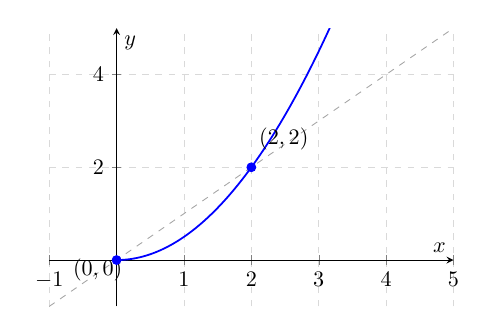
\begin{tikzpicture}[scale=0.8]
    \begin{axis}[
        axis lines = middle,
        xlabel = $x$,
        ylabel = $y$,
        xmin = -1, xmax = 5,
        ymin = -1, ymax = 5,
        grid = major,
        grid style = {dashed, gray!30},
        width = 8cm,
        height = 6cm,
    ]
    \addplot[domain=-1:5, dashed, gray!70, thin] {x};
    
    \addplot[domain=0:4, samples=100, thick, blue] {x^2/2};
    \addplot[mark=*, mark size=2pt, blue] coordinates {(0,0)};
    \addplot[mark=*, mark size=2pt, blue] coordinates {(2,2)};
    \node[anchor=south west] at (axis cs:2,2.2) {$(2,2)$};
    \node[anchor=north east] at (axis cs:0.2,0.2) {$(0,0)$};
    \end{axis}
\end{tikzpicture}
\end{figure}}

\bigskip

\exercicio{
Na figura está representado o gráfico de uma função $g$. Represente, no referencial dado, o gráfico da função inversa $g^{-1}$.

\begin{figure}[H]
\centering
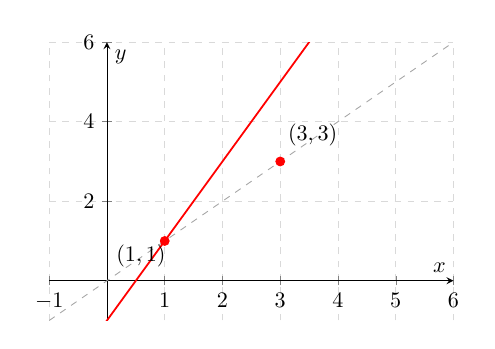
\begin{tikzpicture}[scale=0.8]
    \begin{axis}[
        axis lines = middle,
        xlabel = $x$,
        ylabel = $y$,
        xmin = -1, xmax = 6,
        ymin = -1, ymax = 6,
        grid = major,
        grid style = {dashed, gray!30},
        width = 8cm,
        height = 6cm,
    ]
    \addplot[domain=-1:6, dashed, gray!70, thin] {x};
    
    \addplot[domain=-1:5, thick, red] {2*x-1};
    \addplot[mark=*, mark size=2pt, red] coordinates {(1,1)};
    \addplot[mark=*, mark size=2pt, red] coordinates {(3,3)};
    \node[anchor=south west] at (axis cs:3,3.2) {$(3,3)$};
    \node[anchor=north east] at (axis cs:1.15,1.1) {$(1,1)$};
    \end{axis}
\end{tikzpicture}
\end{figure}
\vspace{3cm}}
\FloatBarrier

% Exercise ID: MAT_P4FUNCOE_4FIN_GRA_001
% Module: MÓDULO P4 - Funções | Concept: Função Inversa | Type: Determinação Gráfica
% Difficulty: 2/5 (Fácil) | Type: desenvolvimento
% Points: 10 | Time: 10 min
% Tags: inversa, grafico, simetria, funcao_quadratica
% Author: Professor | Date: 2025-11-18
% Status: active
% Description: Dado o gráfico de ramos de funções, desenhar o gráfico da inversa

\exercicio
Na figura está representado o gráfico de uma função $f$ definida em $[0, +\infty[$. Represente, no referencial dado, o gráfico da função inversa $f^{-1}$.

\begin{figure}[ht]
\centering
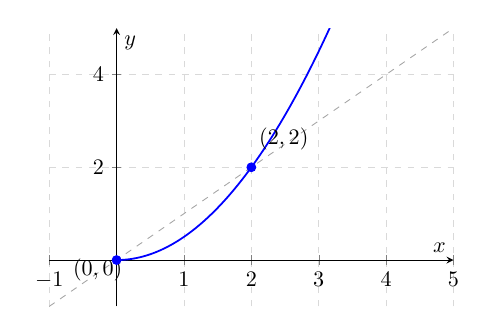
\begin{tikzpicture}[scale=0.8]
    \begin{axis}[
        axis lines = middle,
        xlabel = $x$,
        ylabel = $y$,
        xmin = -1, xmax = 5,
        ymin = -1, ymax = 5,
        grid = major,
        grid style = {dashed, gray!30},
        width = 8cm,
        height = 6cm,
    ]
    \addplot[domain=-1:5, dashed, gray!70, thin] {x};
    
    \addplot[domain=0:4, samples=100, thick, blue] {x^2/2};
    \addplot[mark=*, mark size=2pt, blue] coordinates {(0,0)};
    \addplot[mark=*, mark size=2pt, blue] coordinates {(2,2)};
    \node[anchor=south west] at (axis cs:2,2.2) {$(2,2)$};
    \node[anchor=north east] at (axis cs:0.2,0.2) {$(0,0)$};
    \end{axis}
\end{tikzpicture}
\end{figure}

\bigskip

\exercicio
Na figura está representado o gráfico de uma função $g$. Represente, no referencial dado, o gráfico da função inversa $g^{-1}$.

\begin{figure}[H]
\centering
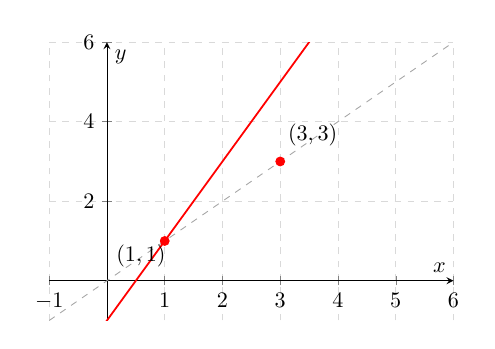
\begin{tikzpicture}[scale=0.8]
    \begin{axis}[
        axis lines = middle,
        xlabel = $x$,
        ylabel = $y$,
        xmin = -1, xmax = 6,
        ymin = -1, ymax = 6,
        grid = major,
        grid style = {dashed, gray!30},
        width = 8cm,
        height = 6cm,
    ]
    \addplot[domain=-1:6, dashed, gray!70, thin] {x};
    
    \addplot[domain=-1:5, thick, red] {2*x-1};
    \addplot[mark=*, mark size=2pt, red] coordinates {(1,1)};
    \addplot[mark=*, mark size=2pt, red] coordinates {(3,3)};
    \node[anchor=south west] at (axis cs:3,3.2) {$(3,3)$};
    \node[anchor=north east] at (axis cs:1.15,1.1) {$(1,1)$};
    \end{axis}
\end{tikzpicture}
\end{figure
\vspace{3cm}
}

\FloatBarrier

% Exercise ID: MAT_P4FUNCOE_4FIN_GRA_001
% Module: MÓDULO P4 - Funções | Concept: Função Inversa | Type: Determinação Gráfica
% Difficulty: 2/5 (Fácil) | Type: desenvolvimento
% Points: 10 | Time: 10 min
% Tags: inversa, grafico, simetria, funcao_quadratica
% Author: Professor | Date: 2025-11-18
% Status: active
% Description: Dado o gráfico de ramos de funções, desenhar o gráfico da inversa

\exercicio{
Na figura está representado o gráfico de uma função $f$ definida em $[0, +\infty[$. Represente, no referencial dado, o gráfico da função inversa $f^{-1}$.

\begin{figure}[ht]
\centering
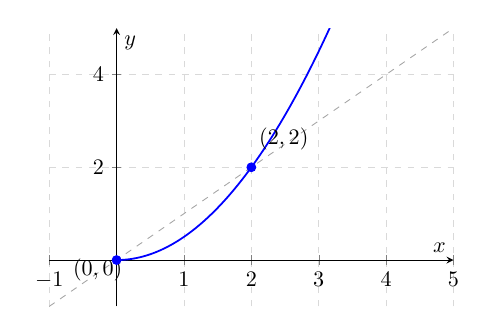
\begin{tikzpicture}[scale=0.8]
    \begin{axis}[
        axis lines = middle,
        xlabel = $x$,
        ylabel = $y$,
        xmin = -1, xmax = 5,
        ymin = -1, ymax = 5,
        grid = major,
        grid style = {dashed, gray!30},
        width = 8cm,
        height = 6cm,
    ]
    \addplot[domain=-1:5, dashed, gray!70, thin] {x};
    
    \addplot[domain=0:4, samples=100, thick, blue] {x^2/2};
    \addplot[mark=*, mark size=2pt, blue] coordinates {(0,0)};
    \addplot[mark=*, mark size=2pt, blue] coordinates {(2,2)};
    \node[anchor=south west] at (axis cs:2,2.2) {$(2,2)$};
    \node[anchor=north east] at (axis cs:0.2,0.2) {$(0,0)$};
    \end{axis}
\end{tikzpicture}
\end{figure}}

\bigskip

\exercicio{
Na figura está representado o gráfico de uma função $g$. Represente, no referencial dado, o gráfico da função inversa $g^{-1}$.

\begin{figure}[H]
\centering
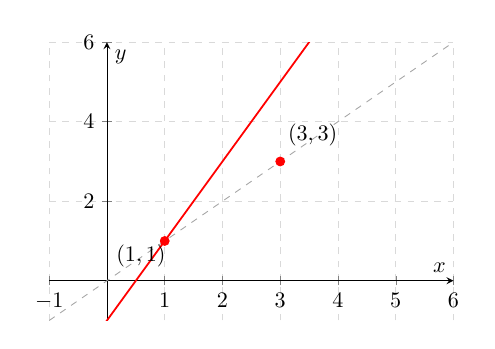
\begin{tikzpicture}[scale=0.8]
    \begin{axis}[
        axis lines = middle,
        xlabel = $x$,
        ylabel = $y$,
        xmin = -1, xmax = 6,
        ymin = -1, ymax = 6,
        grid = major,
        grid style = {dashed, gray!30},
        width = 8cm,
        height = 6cm,
    ]
    \addplot[domain=-1:6, dashed, gray!70, thin] {x};
    
    \addplot[domain=-1:5, thick, red] {2*x-1};
    \addplot[mark=*, mark size=2pt, red] coordinates {(1,1)};
    \addplot[mark=*, mark size=2pt, red] coordinates {(3,3)};
    \node[anchor=south west] at (axis cs:3,3.2) {$(3,3)$};
    \node[anchor=north east] at (axis cs:1.15,1.1) {$(1,1)$};
    \end{axis}
\end{tikzpicture}
\end{figure}}
\vspace{3cm}



\FloatBarrier

% Exercise ID: MAT_P4FUNCOE_4FIN_GRA_002
% Exercise ID: MAT_P4FUNCOE_4FIN_GRA_002
% Module: MÓDULO P4 - Funções | Concept: Função Inversa | Type: Determinação Gráfica
% Difficulty: 2/5 (Fácil) | Type: desenvolvimento
% Points: 10 | Time: 10 min
% Tags: inversa, grafico, simetria, funcao_quadratica
% Author: Professor | Date: 2025-11-18
% Status: active
% Description: Dado o gráfico de ramos de funções, desenhar o gráfico da inversa

\exercicio
Na figura está representado o gráfico de uma função $h$ definida em $]-\infty, 0]$. Represente, no referencial dado, o gráfico da função inversa $h^{-1}$.

\begin{figure}[ht]
\centering
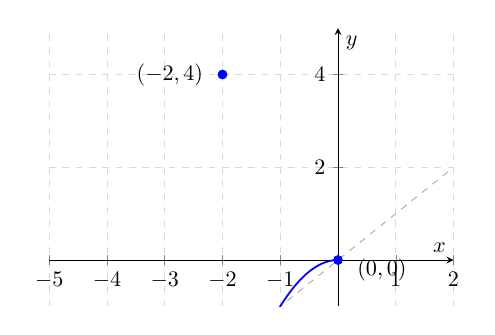
\begin{tikzpicture}[scale=0.8]
    \begin{axis}[
        axis lines = middle,
        xlabel = $x$,
        ylabel = $y$,
        xmin = -5, xmax = 2,
        ymin = -1, ymax = 5,
        grid = major,
        grid style = {dashed, gray!30},
        width = 8cm,
        height = 6cm,
    ]
    \addplot[domain=-5:5, dashed, gray!70, thin] {x};
    
    \addplot[domain=-4:0, samples=100, thick, blue] {-x^2};
    \addplot[mark=*, mark size=2pt, blue] coordinates {(0,0)};
    \addplot[mark=*, mark size=2pt, blue] coordinates {(-2,4)};
    \node[anchor=east] at (axis cs:-2.2,4) {$(-2,4)$};
    \node[anchor=north west] at (axis cs:0.2,0.2) {$(0,0)$};
    \end{axis}
\end{tikzpicture}
\end{figure}

\bigskip

\exercicio
Na figura está representado o gráfico de uma função $k$ definida em $[1, 5]$. Represente, no referencial dado, o gráfico da função inversa $k^{-1}$.

\begin{figure}[H]
\centering
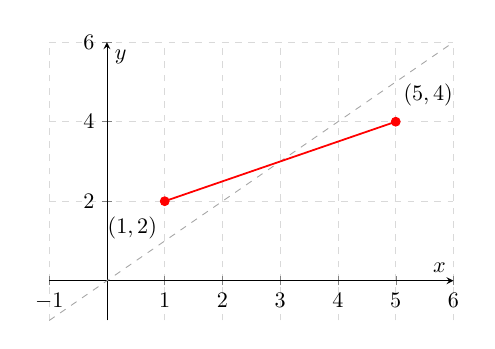
\begin{tikzpicture}[scale=0.8]
    \begin{axis}[
        axis lines = middle,
        xlabel = $x$,
        ylabel = $y$,
        xmin = -1, xmax = 6,
        ymin = -1, ymax = 6,
        grid = major,
        grid style = {dashed, gray!30},
        width = 8cm,
        height = 6cm,
    ]
    \addplot[domain=-1:6, dashed, gray!70, thin] {x};
    
    \addplot[domain=1:5, thick, red] {0.5*x+1.5};
    \addplot[mark=*, mark size=2pt, red] coordinates {(1,2)};
    \addplot[mark=*, mark size=2pt, red] coordinates {(5,4)};
    \node[anchor=south west] at (axis cs:5,4.2) {$(5,4)$};
    \node[anchor=north east] at (axis cs:1,1.8) {$(1,2)$};
    \end{axis}
\end{tikzpicture}
\end{figure}
\vspace{3cm}
}
\FloatBarrier

% Exercise ID: MAT_P4FUNCOE_4FIN_GRA_002
% Exercise ID: MAT_P4FUNCOE_4FIN_GRA_002
% Module: MÓDULO P4 - Funções | Concept: Função Inversa | Type: Determinação Gráfica
% Difficulty: 2/5 (Fácil) | Type: desenvolvimento
% Points: 10 | Time: 10 min
% Tags: inversa, grafico, simetria, funcao_quadratica
% Author: Professor | Date: 2025-11-18
% Status: active
% Description: Dado o gráfico de ramos de funções, desenhar o gráfico da inversa

\exercicio
Na figura está representado o gráfico de uma função $h$ definida em $]-\infty, 0]$. Represente, no referencial dado, o gráfico da função inversa $h^{-1}$.

\begin{figure}[ht]
\centering
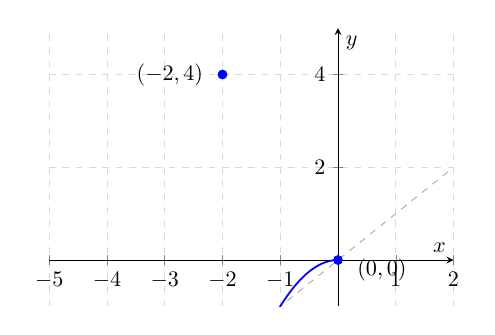
\begin{tikzpicture}[scale=0.8]
    \begin{axis}[
        axis lines = middle,
        xlabel = $x$,
        ylabel = $y$,
        xmin = -5, xmax = 2,
        ymin = -1, ymax = 5,
        grid = major,
        grid style = {dashed, gray!30},
        width = 8cm,
        height = 6cm,
    ]
    \addplot[domain=-5:5, dashed, gray!70, thin] {x};
    
    \addplot[domain=-4:0, samples=100, thick, blue] {-x^2};
    \addplot[mark=*, mark size=2pt, blue] coordinates {(0,0)};
    \addplot[mark=*, mark size=2pt, blue] coordinates {(-2,4)};
    \node[anchor=east] at (axis cs:-2.2,4) {$(-2,4)$};
    \node[anchor=north west] at (axis cs:0.2,0.2) {$(0,0)$};
    \end{axis}
\end{tikzpicture}
\end{figure}

\bigskip

\exercicio
Na figura está representado o gráfico de uma função $k$ definida em $[1, 5]$. Represente, no referencial dado, o gráfico da função inversa $k^{-1}$.

\begin{figure}[H]
\centering
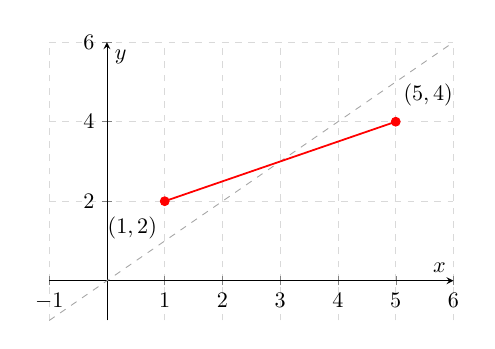
\begin{tikzpicture}[scale=0.8]
    \begin{axis}[
        axis lines = middle,
        xlabel = $x$,
        ylabel = $y$,
        xmin = -1, xmax = 6,
        ymin = -1, ymax = 6,
        grid = major,
        grid style = {dashed, gray!30},
        width = 8cm,
        height = 6cm,
    ]
    \addplot[domain=-1:6, dashed, gray!70, thin] {x};
    
    \addplot[domain=1:5, thick, red] {0.5*x+1.5};
    \addplot[mark=*, mark size=2pt, red] coordinates {(1,2)};
    \addplot[mark=*, mark size=2pt, red] coordinates {(5,4)};
    \node[anchor=south west] at (axis cs:5,4.2) {$(5,4)$};
    \node[anchor=north east] at (axis cs:1,1.8) {$(1,2)$};
    \end{axis}
\end{tikzpicture}
\end{figure
\vspace{3cm}
}

\FloatBarrier

% Exercise ID: MAT_P4FUNCOE_4FIN_GRA_002
% Exercise ID: MAT_P4FUNCOE_4FIN_GRA_002
% Module: MÓDULO P4 - Funções | Concept: Função Inversa | Type: Determinação Gráfica
% Difficulty: 2/5 (Fácil) | Type: desenvolvimento
% Points: 10 | Time: 10 min
% Tags: inversa, grafico, simetria, funcao_quadratica
% Author: Professor | Date: 2025-11-18
% Status: active
% Description: Dado o gráfico de ramos de funções, desenhar o gráfico da inversa

\exercicio
Na figura está representado o gráfico de uma função $h$ definida em $]-\infty, 0]$. Represente, no referencial dado, o gráfico da função inversa $h^{-1}$.

\begin{figure}[ht]
\centering
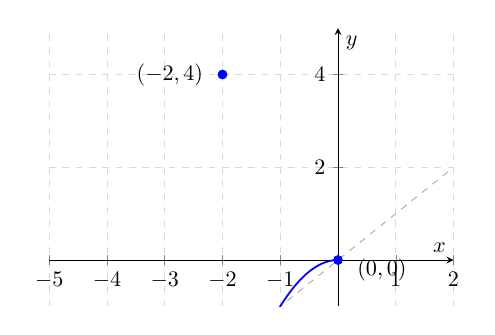
\begin{tikzpicture}[scale=0.8]
    \begin{axis}[
        axis lines = middle,
        xlabel = $x$,
        ylabel = $y$,
        xmin = -5, xmax = 2,
        ymin = -1, ymax = 5,
        grid = major,
        grid style = {dashed, gray!30},
        width = 8cm,
        height = 6cm,
    ]
    \addplot[domain=-5:5, dashed, gray!70, thin] {x};
    
    \addplot[domain=-4:0, samples=100, thick, blue] {-x^2};
    \addplot[mark=*, mark size=2pt, blue] coordinates {(0,0)};
    \addplot[mark=*, mark size=2pt, blue] coordinates {(-2,4)};
    \node[anchor=east] at (axis cs:-2.2,4) {$(-2,4)$};
    \node[anchor=north west] at (axis cs:0.2,0.2) {$(0,0)$};
    \end{axis}
\end{tikzpicture}
\end{figure}

\bigskip

\exercicio
Na figura está representado o gráfico de uma função $k$ definida em $[1, 5]$. Represente, no referencial dado, o gráfico da função inversa $k^{-1}$.

\begin{figure}[H]
\centering
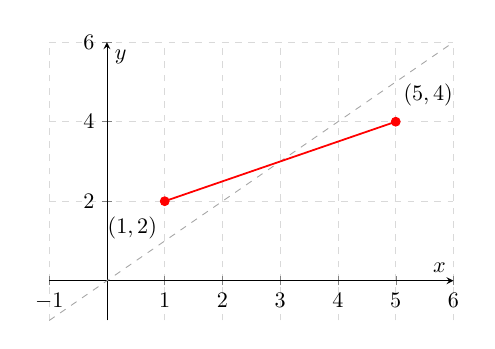
\begin{tikzpicture}[scale=0.8]
    \begin{axis}[
        axis lines = middle,
        xlabel = $x$,
        ylabel = $y$,
        xmin = -1, xmax = 6,
        ymin = -1, ymax = 6,
        grid = major,
        grid style = {dashed, gray!30},
        width = 8cm,
        height = 6cm,
    ]
    \addplot[domain=-1:6, dashed, gray!70, thin] {x};
    
    \addplot[domain=1:5, thick, red] {0.5*x+1.5};
    \addplot[mark=*, mark size=2pt, red] coordinates {(1,2)};
    \addplot[mark=*, mark size=2pt, red] coordinates {(5,4)};
    \node[anchor=south west] at (axis cs:5,4.2) {$(5,4)$};
    \node[anchor=north east] at (axis cs:1,1.8) {$(1,2)$};
    \end{axis}
\end{tikzpicture}
\end{figure}
\vspace{3cm}



\FloatBarrier

% Exercise ID: MAT_P4FUNCOE_4FIN_GRA_003
% Exercise ID: MAT_P4FUNCOE_4FIN_GRA_003
% Module: MÓDULO P4 - Funções | Concept: Função Inversa | Type: Determinação Gráfica
% Difficulty: 2/5 (Fácil) | Type: desenvolvimento
% Points: 10 | Time: 10 min
% Tags: inversa, grafico, simetria, funcao_quadratica
% Author: Professor | Date: 2025-11-18
% Status: active
% Description: Dado o gráfico de ramos de funções, desenhar o gráfico da inversa

\exercicio
Na figura está representado o gráfico de uma função $f$ definida em $[0, +\infty[$. Represente, no referencial dado, o gráfico da função inversa $f^{-1}$.

\begin{figure}[ht]
\centering
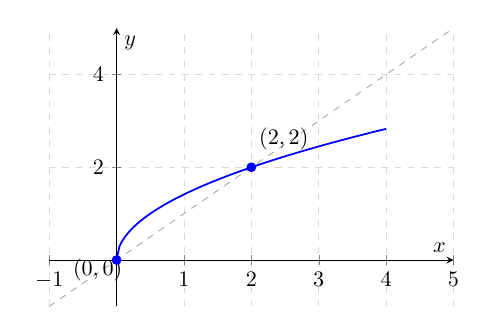
\begin{tikzpicture}[scale=0.8]
    \begin{axis}[
        axis lines = middle,
        xlabel = $x$,
        ylabel = $y$,
        xmin = -1, xmax = 5,
        ymin = -1, ymax = 5,
        grid = major,
        grid style = {dashed, gray!30},
        width = 8cm,
        height = 6cm,
    ]
    \addplot[domain=-1:5, dashed, gray!70, thin] {x};
    
    \addplot[domain=0:4, samples=100, thick, blue] {sqrt(2*x)};
    \addplot[mark=*, mark size=2pt, blue] coordinates {(0,0)};
    \addplot[mark=*, mark size=2pt, blue] coordinates {(2,2)};
    \node[anchor=south west] at (axis cs:2,2.2) {$(2,2)$};
    \node[anchor=north east] at (axis cs:0.2,0.2) {$(0,0)$};
    \end{axis}
\end{tikzpicture}
\end{figure}

\bigskip

\exercicio
Na figura está representado o gráfico de uma função $g$ definida em $[-1, 3]$. Represente, no referencial dado, o gráfico da função inversa $g^{-1}$.

\begin{figure}[H]
\centering
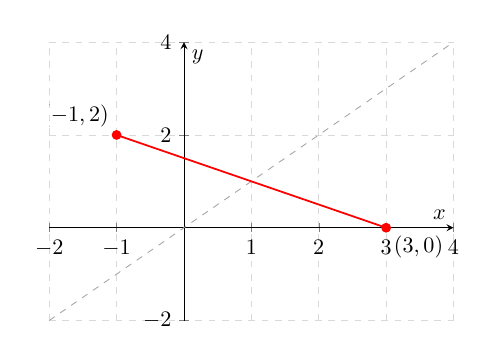
\begin{tikzpicture}[scale=0.8]
    \begin{axis}[
        axis lines = middle,
        xlabel = $x$,
        ylabel = $y$,
        xmin = -2, xmax = 4,
        ymin = -2, ymax = 4,
        grid = major,
        grid style = {dashed, gray!30},
        width = 8cm,
        height = 6cm,
    ]
    \addplot[domain=-2:4, dashed, gray!70, thin] {x};
    
    \addplot[domain=-1:3, thick, red] {-0.5*x+1.5};
    \addplot[mark=*, mark size=2pt, red] coordinates {(-1,2)};
    \addplot[mark=*, mark size=2pt, red] coordinates {(3,0)};
    \node[anchor=south east] at (axis cs:-1,2) {$(-1,2)$};
    \node[anchor=north west] at (axis cs:3,0) {$(3,0)$};
    \end{axis}
\end{tikzpicture}
\end{figure}
\vspace{3cm}
}
\FloatBarrier

% Exercise ID: MAT_P4FUNCOE_4FIN_GRA_003
% Exercise ID: MAT_P4FUNCOE_4FIN_GRA_003
% Module: MÓDULO P4 - Funções | Concept: Função Inversa | Type: Determinação Gráfica
% Difficulty: 2/5 (Fácil) | Type: desenvolvimento
% Points: 10 | Time: 10 min
% Tags: inversa, grafico, simetria, funcao_quadratica
% Author: Professor | Date: 2025-11-18
% Status: active
% Description: Dado o gráfico de ramos de funções, desenhar o gráfico da inversa

\exercicio
Na figura está representado o gráfico de uma função $f$ definida em $[0, +\infty[$. Represente, no referencial dado, o gráfico da função inversa $f^{-1}$.

\begin{figure}[ht]
\centering
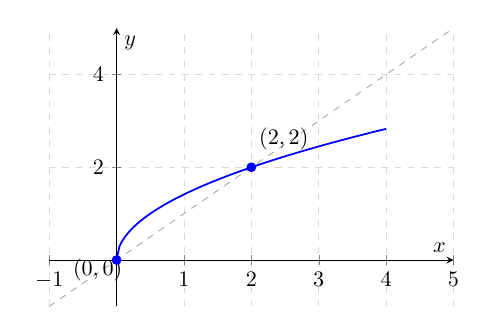
\begin{tikzpicture}[scale=0.8]
    \begin{axis}[
        axis lines = middle,
        xlabel = $x$,
        ylabel = $y$,
        xmin = -1, xmax = 5,
        ymin = -1, ymax = 5,
        grid = major,
        grid style = {dashed, gray!30},
        width = 8cm,
        height = 6cm,
    ]
    \addplot[domain=-1:5, dashed, gray!70, thin] {x};
    
    \addplot[domain=0:4, samples=100, thick, blue] {sqrt(2*x)};
    \addplot[mark=*, mark size=2pt, blue] coordinates {(0,0)};
    \addplot[mark=*, mark size=2pt, blue] coordinates {(2,2)};
    \node[anchor=south west] at (axis cs:2,2.2) {$(2,2)$};
    \node[anchor=north east] at (axis cs:0.2,0.2) {$(0,0)$};
    \end{axis}
\end{tikzpicture}
\end{figure}

\bigskip

\exercicio
Na figura está representado o gráfico de uma função $g$ definida em $[-1, 3]$. Represente, no referencial dado, o gráfico da função inversa $g^{-1}$.

\begin{figure}[H]
\centering
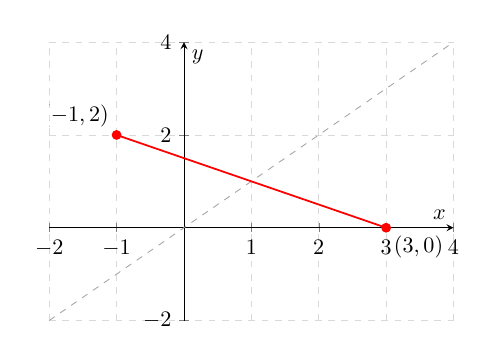
\begin{tikzpicture}[scale=0.8]
    \begin{axis}[
        axis lines = middle,
        xlabel = $x$,
        ylabel = $y$,
        xmin = -2, xmax = 4,
        ymin = -2, ymax = 4,
        grid = major,
        grid style = {dashed, gray!30},
        width = 8cm,
        height = 6cm,
    ]
    \addplot[domain=-2:4, dashed, gray!70, thin] {x};
    
    \addplot[domain=-1:3, thick, red] {-0.5*x+1.5};
    \addplot[mark=*, mark size=2pt, red] coordinates {(-1,2)};
    \addplot[mark=*, mark size=2pt, red] coordinates {(3,0)};
    \node[anchor=south east] at (axis cs:-1,2) {$(-1,2)$};
    \node[anchor=north west] at (axis cs:3,0) {$(3,0)$};
    \end{axis}
\end{tikzpicture}
\end{figure
\vspace{3cm}
}

\FloatBarrier

% Exercise ID: MAT_P4FUNCOE_4FIN_GRA_003
% Exercise ID: MAT_P4FUNCOE_4FIN_GRA_003
% Module: MÓDULO P4 - Funções | Concept: Função Inversa | Type: Determinação Gráfica
% Difficulty: 2/5 (Fácil) | Type: desenvolvimento
% Points: 10 | Time: 10 min
% Tags: inversa, grafico, simetria, funcao_quadratica
% Author: Professor | Date: 2025-11-18
% Status: active
% Description: Dado o gráfico de ramos de funções, desenhar o gráfico da inversa

\exercicio{
Na figura está representado o gráfico de uma função $f$ definida em $[0, +\infty[$. Represente, no referencial dado, o gráfico da função inversa $f^{-1}$.

\begin{figure}[ht]
\centering
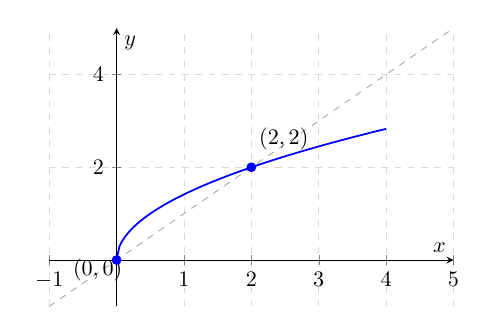
\begin{tikzpicture}[scale=0.8]
    \begin{axis}[
        axis lines = middle,
        xlabel = $x$,
        ylabel = $y$,
        xmin = -1, xmax = 5,
        ymin = -1, ymax = 5,
        grid = major,
        grid style = {dashed, gray!30},
        width = 8cm,
        height = 6cm,
    ]
    \addplot[domain=-1:5, dashed, gray!70, thin] {x};
    
    \addplot[domain=0:4, samples=100, thick, blue] {sqrt(2*x)};
    \addplot[mark=*, mark size=2pt, blue] coordinates {(0,0)};
    \addplot[mark=*, mark size=2pt, blue] coordinates {(2,2)};
    \node[anchor=south west] at (axis cs:2,2.2) {$(2,2)$};
    \node[anchor=north east] at (axis cs:0.2,0.2) {$(0,0)$};
    \end{axis}
\end{tikzpicture}
\end{figure}}

\bigskip

\exercicio{
Na figura está representado o gráfico de uma função $g$ definida em $[-1, 3]$. Represente, no referencial dado, o gráfico da função inversa $g^{-1}$.

\begin{figure}[H]
\centering
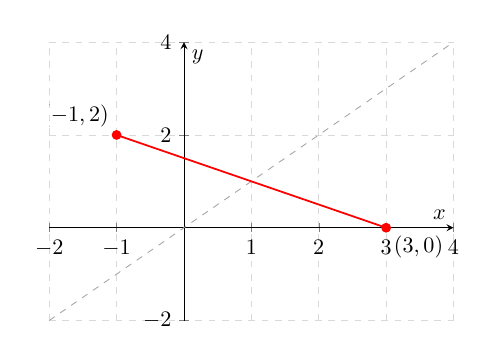
\begin{tikzpicture}[scale=0.8]
    \begin{axis}[
        axis lines = middle,
        xlabel = $x$,
        ylabel = $y$,
        xmin = -2, xmax = 4,
        ymin = -2, ymax = 4,
        grid = major,
        grid style = {dashed, gray!30},
        width = 8cm,
        height = 6cm,
    ]
    \addplot[domain=-2:4, dashed, gray!70, thin] {x};
    
    \addplot[domain=-1:3, thick, red] {-0.5*x+1.5};
    \addplot[mark=*, mark size=2pt, red] coordinates {(-1,2)};
    \addplot[mark=*, mark size=2pt, red] coordinates {(3,0)};
    \node[anchor=south east] at (axis cs:-1,2) {$(-1,2)$};
    \node[anchor=north west] at (axis cs:3,0) {$(3,0)$};
    \end{axis}
\end{tikzpicture}
\end{figure}}

\vspace{3cm}
\FloatBarrier

% Exercise ID: MAT_P4FUNCOE_4FIN_GRA_004
% Exercise ID: MAT_P4FUNCOE_4FIN_GRA_004
% Module: MÓDULO P4 - Funções | Concept: Função Inversa | Type: Determinação Gráfica
% Difficulty: 2/5 (Fácil) | Type: desenvolvimento
% Points: 10 | Time: 10 min
% Tags: inversa, grafico, simetria, funcao_quadratica
% Author: Professor | Date: 2025-11-18
% Status: active
% Description: Dado o gráfico de ramos de funções, desenhar o gráfico da inversa

\exercicio
Na figura está representado o gráfico de uma função $f$ definida em $[1, 4]$. Represente, no referencial dado, o gráfico da função inversa $f^{-1}$.

\begin{figure}[ht]
\centering
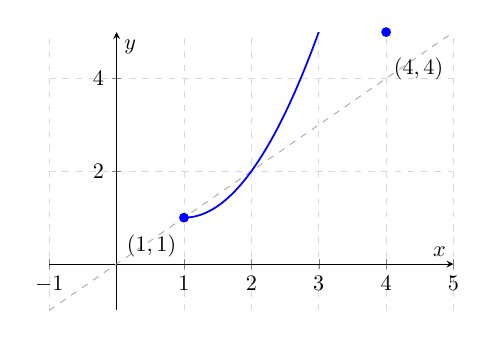
\begin{tikzpicture}[scale=0.8]
    \begin{axis}[
        axis lines = middle,
        xlabel = $x$,
        ylabel = $y$,
        xmin = -1, xmax = 5,
        ymin = -1, ymax = 5,
        grid = major,
        grid style = {dashed, gray!30},
        width = 8cm,
        height = 6cm,
    ]
    \addplot[domain=-1:5, dashed, gray!70, thin] {x};
    
    \addplot[domain=1:4, samples=100, thick, blue] {(x-1)^2 + 1};
    \addplot[mark=*, mark size=2pt, blue] coordinates {(1,1)};
    \addplot[mark=*, mark size=2pt, blue] coordinates {(4,10/2)};
    \node[anchor=west] at (axis cs:4,4.2) {$(4,4)$};
    \node[anchor=north east] at (axis cs:1,0.8) {$(1,1)$};
    \end{axis}
\end{tikzpicture}
\end{figure}

\bigskip

\exercicio
Na figura está representado o gráfico de uma função $g$ definida em $]0, 4]$. Represente, no referencial dado, o gráfico da função inversa $g^{-1}$.

\begin{figure}[H]
\centering
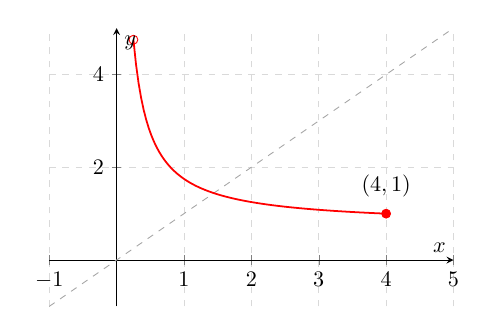
\begin{tikzpicture}[scale=0.8]
    \begin{axis}[
        axis lines = middle,
        xlabel = $x$,
        ylabel = $y$,
        xmin = -1, xmax = 5,
        ymin = -1, ymax = 5,
        grid = major,
        grid style = {dashed, gray!30},
        width = 8cm,
        height = 6cm,
    ]
    \addplot[domain=-1:5, dashed, gray!70, thin] {x};
    
    \addplot[domain=0.25:4, samples=100, thick, red] {1/x + 0.75};
    \addplot[mark=o, mark size=2pt, red] coordinates {(0.25,4.75)};
    \addplot[mark=*, mark size=2pt, red] coordinates {(4,1)};
    \node[anchor=south] at (axis cs:4,1.2) {$(4,1)$};
    \end{axis}
\end{tikzpicture}
\end{figure}
\vspace{3cm}
}
\FloatBarrier

% Exercise ID: MAT_P4FUNCOE_4FIN_GRA_004
% Exercise ID: MAT_P4FUNCOE_4FIN_GRA_004
% Module: MÓDULO P4 - Funções | Concept: Função Inversa | Type: Determinação Gráfica
% Difficulty: 2/5 (Fácil) | Type: desenvolvimento
% Points: 10 | Time: 10 min
% Tags: inversa, grafico, simetria, funcao_quadratica
% Author: Professor | Date: 2025-11-18
% Status: active
% Description: Dado o gráfico de ramos de funções, desenhar o gráfico da inversa

\exercicio
Na figura está representado o gráfico de uma função $f$ definida em $[1, 4]$. Represente, no referencial dado, o gráfico da função inversa $f^{-1}$.

\begin{figure}[ht]
\centering
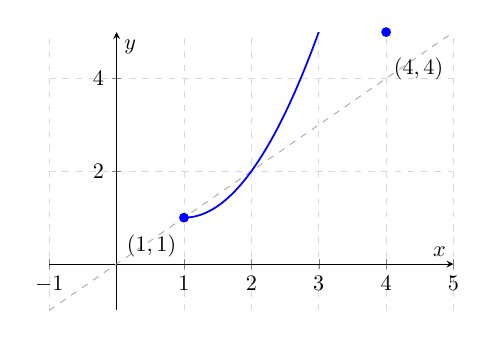
\begin{tikzpicture}[scale=0.8]
    \begin{axis}[
        axis lines = middle,
        xlabel = $x$,
        ylabel = $y$,
        xmin = -1, xmax = 5,
        ymin = -1, ymax = 5,
        grid = major,
        grid style = {dashed, gray!30},
        width = 8cm,
        height = 6cm,
    ]
    \addplot[domain=-1:5, dashed, gray!70, thin] {x};
    
    \addplot[domain=1:4, samples=100, thick, blue] {(x-1)^2 + 1};
    \addplot[mark=*, mark size=2pt, blue] coordinates {(1,1)};
    \addplot[mark=*, mark size=2pt, blue] coordinates {(4,10/2)};
    \node[anchor=west] at (axis cs:4,4.2) {$(4,4)$};
    \node[anchor=north east] at (axis cs:1,0.8) {$(1,1)$};
    \end{axis}
\end{tikzpicture}
\end{figure}

\bigskip

\exercicio
Na figura está representado o gráfico de uma função $g$ definida em $]0, 4]$. Represente, no referencial dado, o gráfico da função inversa $g^{-1}$.

\begin{figure}[H]
\centering
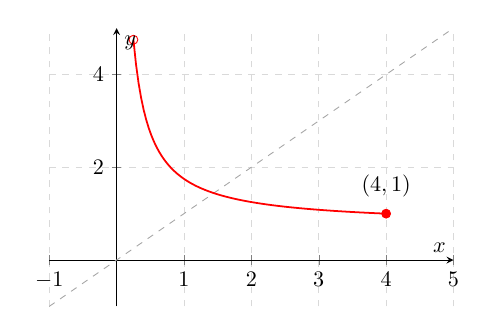
\begin{tikzpicture}[scale=0.8]
    \begin{axis}[
        axis lines = middle,
        xlabel = $x$,
        ylabel = $y$,
        xmin = -1, xmax = 5,
        ymin = -1, ymax = 5,
        grid = major,
        grid style = {dashed, gray!30},
        width = 8cm,
        height = 6cm,
    ]
    \addplot[domain=-1:5, dashed, gray!70, thin] {x};
    
    \addplot[domain=0.25:4, samples=100, thick, red] {1/x + 0.75};
    \addplot[mark=o, mark size=2pt, red] coordinates {(0.25,4.75)};
    \addplot[mark=*, mark size=2pt, red] coordinates {(4,1)};
    \node[anchor=south] at (axis cs:4,1.2) {$(4,1)$};
    \end{axis}
\end{tikzpicture}
\end{figure
\vspace{3cm}
}

\FloatBarrier

% Exercise ID: MAT_P4FUNCOE_4FIN_GRA_004
% Exercise ID: MAT_P4FUNCOE_4FIN_GRA_004
% Module: MÓDULO P4 - Funções | Concept: Função Inversa | Type: Determinação Gráfica
% Difficulty: 2/5 (Fácil) | Type: desenvolvimento
% Points: 10 | Time: 10 min
% Tags: inversa, grafico, simetria, funcao_quadratica
% Author: Professor | Date: 2025-11-18
% Status: active
% Description: Dado o gráfico de ramos de funções, desenhar o gráfico da inversa

\exercicio
Na figura está representado o gráfico de uma função $f$ definida em $[1, 4]$. Represente, no referencial dado, o gráfico da função inversa $f^{-1}$.

\begin{figure}[ht]
\centering
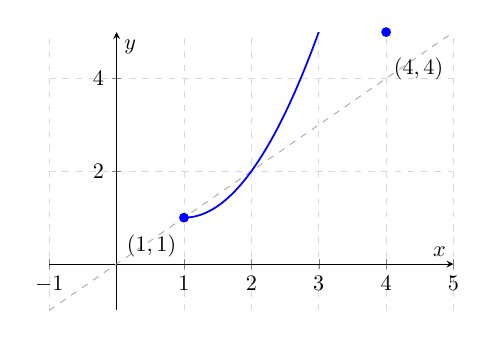
\begin{tikzpicture}[scale=0.8]
    \begin{axis}[
        axis lines = middle,
        xlabel = $x$,
        ylabel = $y$,
        xmin = -1, xmax = 5,
        ymin = -1, ymax = 5,
        grid = major,
        grid style = {dashed, gray!30},
        width = 8cm,
        height = 6cm,
    ]
    \addplot[domain=-1:5, dashed, gray!70, thin] {x};
    
    \addplot[domain=1:4, samples=100, thick, blue] {(x-1)^2 + 1};
    \addplot[mark=*, mark size=2pt, blue] coordinates {(1,1)};
    \addplot[mark=*, mark size=2pt, blue] coordinates {(4,10/2)};
    \node[anchor=west] at (axis cs:4,4.2) {$(4,4)$};
    \node[anchor=north east] at (axis cs:1,0.8) {$(1,1)$};
    \end{axis}
\end{tikzpicture}
\end{figure}

\bigskip

\exercicio
Na figura está representado o gráfico de uma função $g$ definida em $]0, 4]$. Represente, no referencial dado, o gráfico da função inversa $g^{-1}$.

\begin{figure}[H]
\centering
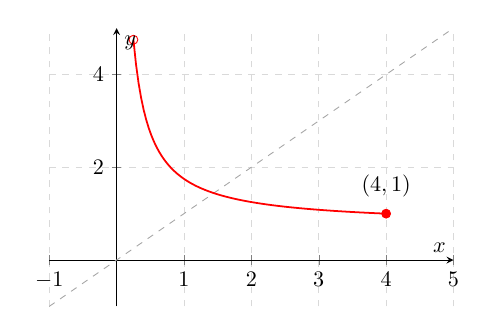
\begin{tikzpicture}[scale=0.8]
    \begin{axis}[
        axis lines = middle,
        xlabel = $x$,
        ylabel = $y$,
        xmin = -1, xmax = 5,
        ymin = -1, ymax = 5,
        grid = major,
        grid style = {dashed, gray!30},
        width = 8cm,
        height = 6cm,
    ]
    \addplot[domain=-1:5, dashed, gray!70, thin] {x};
    
    \addplot[domain=0.25:4, samples=100, thick, red] {1/x + 0.75};
    \addplot[mark=o, mark size=2pt, red] coordinates {(0.25,4.75)};
    \addplot[mark=*, mark size=2pt, red] coordinates {(4,1)};
    \node[anchor=south] at (axis cs:4,1.2) {$(4,1)$};
    \end{axis}
\end{tikzpicture}
\end{figure}
\vspace{3cm}



\FloatBarrier

% Exercise ID: MAT_P4FUNCOE_4FIN_GRA_005
% Exercise ID: MAT_P4FUNCOE_4FIN_GRA_005
% Module: MÓDULO P4 - Funções | Concept: Função Inversa | Type: Determinação Gráfica
% Difficulty: 2/5 (Fácil) | Type: desenvolvimento
% Points: 10 | Time: 10 min
% Tags: inversa, grafico, simetria, funcao_quadratica
% Author: Professor | Date: 2025-11-18
% Status: active
% Description: Dado o gráfico de ramos de funções, desenhar o gráfico da inversa

\exercicio
Na figura está representado o gráfico de uma função $f$ definida em $[-2, 2]$. Represente, no referencial dado, o gráfico da função inversa $f^{-1}$.

\begin{figure}[ht]
\centering
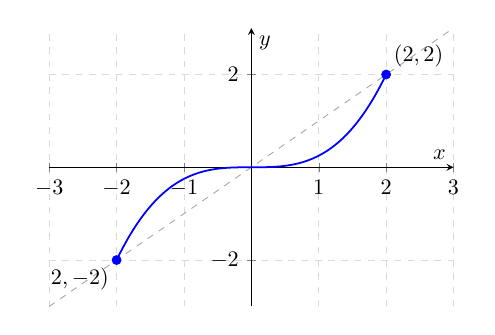
\begin{tikzpicture}[scale=0.8]
    \begin{axis}[
        axis lines = middle,
        xlabel = $x$,
        ylabel = $y$,
        xmin = -3, xmax = 3,
        ymin = -3, ymax = 3,
        grid = major,
        grid style = {dashed, gray!30},
        width = 8cm,
        height = 6cm,
    ]
    \addplot[domain=-3:3, dashed, gray!70, thin] {x};
    
    \addplot[domain=-2:2, samples=100, thick, blue] {x^3/4};
    \addplot[mark=*, mark size=2pt, blue] coordinates {(-2,-2)};
    \addplot[mark=*, mark size=2pt, blue] coordinates {(2,2)};
    \node[anchor=north east] at (axis cs:-2,-2) {$(-2,-2)$};
    \node[anchor=south west] at (axis cs:2,2) {$(2,2)$};
    \end{axis}
\end{tikzpicture}
\end{figure}

\bigskip

\exercicio
Na figura está representado o gráfico de uma função $g$ definida em $[0, 3]$. Represente, no referencial dado, o gráfico da função inversa $g^{-1}$.

\begin{figure}[H]
\centering
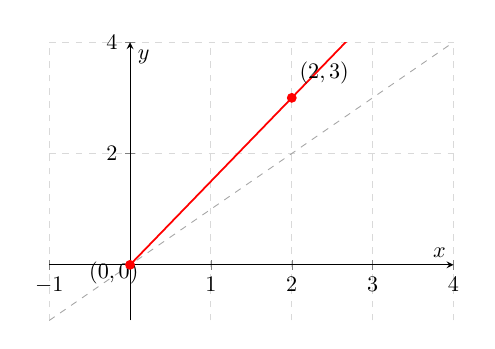
\begin{tikzpicture}[scale=0.8]
    \begin{axis}[
        axis lines = middle,
        xlabel = $x$,
        ylabel = $y$,
        xmin = -1, xmax = 4,
        ymin = -1, ymax = 4,
        grid = major,
        grid style = {dashed, gray!30},
        width = 8cm,
        height = 6cm,
    ]
    \addplot[domain=-1:4, dashed, gray!70, thin] {x};
    
    \addplot[domain=0:3, thick, red] {3*x/2};
    \addplot[mark=*, mark size=2pt, red] coordinates {(0,0)};
    \addplot[mark=*, mark size=2pt, red] coordinates {(2,3)};
    \node[anchor=south west] at (axis cs:2,3.1) {$(2,3)$};
    \node[anchor=north east] at (axis cs:0.2,0.2) {$(0,0)$};
    \end{axis}
\end{tikzpicture}
\end{figure}
\vspace{3cm}
}
\FloatBarrier

% Exercise ID: MAT_P4FUNCOE_4FIN_GRA_005
% Exercise ID: MAT_P4FUNCOE_4FIN_GRA_005
% Module: MÓDULO P4 - Funções | Concept: Função Inversa | Type: Determinação Gráfica
% Difficulty: 2/5 (Fácil) | Type: desenvolvimento
% Points: 10 | Time: 10 min
% Tags: inversa, grafico, simetria, funcao_quadratica
% Author: Professor | Date: 2025-11-18
% Status: active
% Description: Dado o gráfico de ramos de funções, desenhar o gráfico da inversa

\exercicio
Na figura está representado o gráfico de uma função $f$ definida em $[-2, 2]$. Represente, no referencial dado, o gráfico da função inversa $f^{-1}$.

\begin{figure}[ht]
\centering
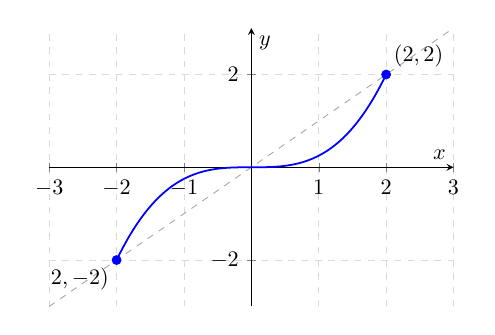
\begin{tikzpicture}[scale=0.8]
    \begin{axis}[
        axis lines = middle,
        xlabel = $x$,
        ylabel = $y$,
        xmin = -3, xmax = 3,
        ymin = -3, ymax = 3,
        grid = major,
        grid style = {dashed, gray!30},
        width = 8cm,
        height = 6cm,
    ]
    \addplot[domain=-3:3, dashed, gray!70, thin] {x};
    
    \addplot[domain=-2:2, samples=100, thick, blue] {x^3/4};
    \addplot[mark=*, mark size=2pt, blue] coordinates {(-2,-2)};
    \addplot[mark=*, mark size=2pt, blue] coordinates {(2,2)};
    \node[anchor=north east] at (axis cs:-2,-2) {$(-2,-2)$};
    \node[anchor=south west] at (axis cs:2,2) {$(2,2)$};
    \end{axis}
\end{tikzpicture}
\end{figure}

\bigskip

\exercicio
Na figura está representado o gráfico de uma função $g$ definida em $[0, 3]$. Represente, no referencial dado, o gráfico da função inversa $g^{-1}$.

\begin{figure}[H]
\centering
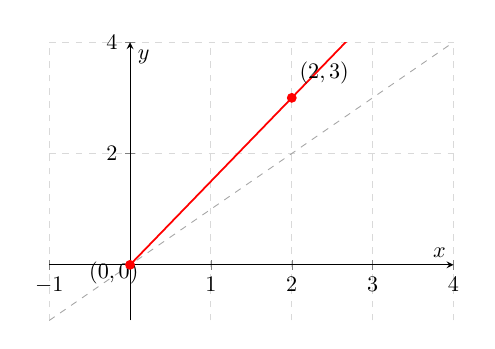
\begin{tikzpicture}[scale=0.8]
    \begin{axis}[
        axis lines = middle,
        xlabel = $x$,
        ylabel = $y$,
        xmin = -1, xmax = 4,
        ymin = -1, ymax = 4,
        grid = major,
        grid style = {dashed, gray!30},
        width = 8cm,
        height = 6cm,
    ]
    \addplot[domain=-1:4, dashed, gray!70, thin] {x};
    
    \addplot[domain=0:3, thick, red] {3*x/2};
    \addplot[mark=*, mark size=2pt, red] coordinates {(0,0)};
    \addplot[mark=*, mark size=2pt, red] coordinates {(2,3)};
    \node[anchor=south west] at (axis cs:2,3.1) {$(2,3)$};
    \node[anchor=north east] at (axis cs:0.2,0.2) {$(0,0)$};
    \end{axis}
\end{tikzpicture}
\end{figure
\vspace{3cm}
}

\FloatBarrier

% Exercise ID: MAT_P4FUNCOE_4FIN_GRA_005
% Exercise ID: MAT_P4FUNCOE_4FIN_GRA_005
% Module: MÓDULO P4 - Funções | Concept: Função Inversa | Type: Determinação Gráfica
% Difficulty: 2/5 (Fácil) | Type: desenvolvimento
% Points: 10 | Time: 10 min
% Tags: inversa, grafico, simetria, funcao_quadratica
% Author: Professor | Date: 2025-11-18
% Status: active
% Description: Dado o gráfico de ramos de funções, desenhar o gráfico da inversa

\exercicio
Na figura está representado o gráfico de uma função $f$ definida em $[-2, 2]$. Represente, no referencial dado, o gráfico da função inversa $f^{-1}$.

\begin{figure}[ht]
\centering
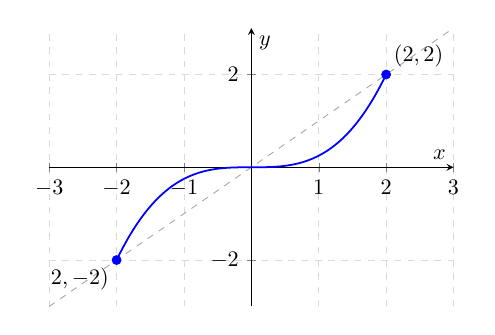
\begin{tikzpicture}[scale=0.8]
    \begin{axis}[
        axis lines = middle,
        xlabel = $x$,
        ylabel = $y$,
        xmin = -3, xmax = 3,
        ymin = -3, ymax = 3,
        grid = major,
        grid style = {dashed, gray!30},
        width = 8cm,
        height = 6cm,
    ]
    \addplot[domain=-3:3, dashed, gray!70, thin] {x};
    
    \addplot[domain=-2:2, samples=100, thick, blue] {x^3/4};
    \addplot[mark=*, mark size=2pt, blue] coordinates {(-2,-2)};
    \addplot[mark=*, mark size=2pt, blue] coordinates {(2,2)};
    \node[anchor=north east] at (axis cs:-2,-2) {$(-2,-2)$};
    \node[anchor=south west] at (axis cs:2,2) {$(2,2)$};
    \end{axis}
\end{tikzpicture}
\end{figure}

\bigskip

\exercicio
Na figura está representado o gráfico de uma função $g$ definida em $[0, 3]$. Represente, no referencial dado, o gráfico da função inversa $g^{-1}$.

\begin{figure}[H]
\centering
\begin{tikzpicture}[scale=0.8]
    \begin{axis}[
        axis lines = middle,
        xlabel = $x$,
        ylabel = $y$,
        xmin = -1, xmax = 4,
        ymin = -1, ymax = 4,
        grid = major,
        grid style = {dashed, gray!30},
        width = 8cm,
        height = 6cm,
    ]
    \addplot[domain=-1:4, dashed, gray!70, thin] {x};
    
    \addplot[domain=0:3, thick, red] {3*x/2};
    \addplot[mark=*, mark size=2pt, red] coordinates {(0,0)};
    \addplot[mark=*, mark size=2pt, red] coordinates {(2,3)};
    \node[anchor=south west] at (axis cs:2,3.1) {$(2,3)$};
    \node[anchor=north east] at (axis cs:0.2,0.2) {$(0,0)$};
    \end{axis}
\end{tikzpicture}
\end{figure}
\vspace{3cm}



\FloatBarrier

% Exercise ID: MAT_P4FUNCOE_4FX_DGX_001
% Module: MÓDULO P4 - Funções | Concept: Função Inversa | Type: Determinação Gráfica da Função Inversa
% Difficulty: 4/5 (Difícil) | Format: standard
% Tags: sobrejetividade, inversa, grafico, representacao_grafica, bissectriz, injetividade, simetria, grafico, simetria
% Author: Test Agent | Date: 2025-11-26
% Status: active

\exercicio{Determine graficamente a função inversa de f(x) = x^2 + 2, para x  0.}

\FloatBarrier

% Exercise ID: MAT_P4FUNCOE_4FIN_TRH_001
% Module: MÓDULO P4 - Funções | Concept: Função Inversa | Type: Teste da Reta Horizontal
% Difficulty: 2/5 (Fácil) | Type: desenvolvimento
% Points: 10 | Time: 10 min
% Tags: inversa, injetividade, teste_reta_horizontal, grafico
% Author: Professor | Date: 2025-11-18
% Status: active
% Description: Determinar quais funções são invertíveis usando teste da reta horizontal

\exercicio
Considere as funções representadas nas figuras seguintes:

\begin{figure}[H]
\centering
\begin{minipage}{0.45\textwidth}
\centering
\begin{tikzpicture}[scale=0.8]
    \begin{axis}[
        axis lines = middle,
        xlabel = $x$,
        ylabel = $y$,
        xmin = -3, xmax = 3,
        ymin = -1, ymax = 4,
        grid = major,
        grid style = {dashed, gray!30},
        width = 8cm,
        height = 6cm,
        title = {Função A},
        title style = {font=\bfseries},
    ]
    \addplot[domain=-2.5:2.5, samples=100, thick, red] {x^2};
    \end{axis}
\end{tikzpicture}
\end{minipage}
\hfill
\begin{minipage}{0.45\textwidth}
\centering
\begin{tikzpicture}[scale=0.8]
    \begin{axis}[
        axis lines = middle,
        xlabel = $x$,
        ylabel = $y$,
        xmin = -1, xmax = 4,
        ymin = -1, ymax = 4,
        grid = major,
        grid style = {dashed, gray!30},
        width = 8cm,
        height = 6cm,
        title = {Função B},
        title style = {font=\bfseries},
    ]
    \addplot[domain=0:3, samples=100, thick, blue] {x};
    \addplot[mark=*, mark size=2pt, blue] coordinates {(0,0)};
    \addplot[mark=*, mark size=2pt, blue] coordinates {(3,3)};
    \end{axis}
\end{tikzpicture}
\end{minipage}
\end{figure}

Quais das duas funções são invertíveis (isto é, cuja inversa também é uma função)? Justifique usando o teste da reta horizontal.

\vspace{3cm}
\FloatBarrier

% Exercise ID: MAT_P4FUNCOE_4FIN_TRH_001
% Module: MÓDULO P4 - Funções | Concept: Função Inversa | Type: Teste da Reta Horizontal
% Difficulty: 2/5 (Fácil) | Type: desenvolvimento
% Points: 10 | Time: 10 min
% Tags: inversa, injetividade, teste_reta_horizontal, grafico
% Author: Professor | Date: 2025-11-18
% Status: active
% Description: Determinar quais funções são invertíveis usando teste da reta horizontal

\exercicio
Considere as funções representadas nas figuras seguintes:

\begin{figure}[H]
\centering
\begin{minipage}{0.45\textwidth}
\centering
\begin{tikzpicture}[scale=0.8]
    \begin{axis}[
        axis lines = middle,
        xlabel = $x$,
        ylabel = $y$,
        xmin = -3, xmax = 3,
        ymin = -1, ymax = 4,
        grid = major,
        grid style = {dashed, gray!30},
        width = 8cm,
        height = 6cm,
        title = {Função A},
        title style = {font=\bfseries},
    ]
    \addplot[domain=-2.5:2.5, samples=100, thick, red] {x^2};
    \end{axis}
\end{tikzpicture}
\end{minipage}
\hfill
\begin{minipage}{0.45\textwidth}
\centering
\begin{tikzpicture}[scale=0.8]
    \begin{axis}[
        axis lines = middle,
        xlabel = $x$,
        ylabel = $y$,
        xmin = -1, xmax = 4,
        ymin = -1, ymax = 4,
        grid = major,
        grid style = {dashed, gray!30},
        width = 8cm,
        height = 6cm,
        title = {Função B},
        title style = {font=\bfseries},
    ]
    \addplot[domain=0:3, samples=100, thick, blue] {x};
    \addplot[mark=*, mark size=2pt, blue] coordinates {(0,0)};
    \addplot[mark=*, mark size=2pt, blue] coordinates {(3,3)};
    \end{axis}
\end{tikzpicture}
\end{minipage}
\end{figure}

Quais das duas funções são invertíveis (isto é, cuja inversa também é uma função)? Justifique usando o teste da reta horizontal.

\vspace{3cm}

\FloatBarrier

% Exercise ID: MAT_P4FUNCOE_4FIN_TRH_001
% Module: MÓDULO P4 - Funções | Concept: Função Inversa | Type: Teste da Reta Horizontal
% Difficulty: 2/5 (Fácil) | Type: desenvolvimento
% Points: 10 | Time: 10 min
% Tags: inversa, injetividade, teste_reta_horizontal, grafico
% Author: Professor | Date: 2025-11-18
% Status: active
% Description: Determinar quais funções são invertíveis usando teste da reta horizontal

\exercicio
Considere as funções representadas nas figuras seguintes:

\begin{figure}[H]
\centering
\begin{minipage}{0.45\textwidth}
\centering
\begin{tikzpicture}[scale=0.8]
    \begin{axis}[
        axis lines = middle,
        xlabel = $x$,
        ylabel = $y$,
        xmin = -3, xmax = 3,
        ymin = -1, ymax = 4,
        grid = major,
        grid style = {dashed, gray!30},
        width = 8cm,
        height = 6cm,
        title = {Função A},
        title style = {font=\bfseries},
    ]
    \addplot[domain=-2.5:2.5, samples=100, thick, red] {x^2};
    \end{axis}
\end{tikzpicture}
\end{minipage}
\hfill
\begin{minipage}{0.45\textwidth}
\centering
\begin{tikzpicture}[scale=0.8]
    \begin{axis}[
        axis lines = middle,
        xlabel = $x$,
        ylabel = $y$,
        xmin = -1, xmax = 4,
        ymin = -1, ymax = 4,
        grid = major,
        grid style = {dashed, gray!30},
        width = 8cm,
        height = 6cm,
        title = {Função B},
        title style = {font=\bfseries},
    ]
    \addplot[domain=0:3, samples=100, thick, blue] {x};
    \addplot[mark=*, mark size=2pt, blue] coordinates {(0,0)};
    \addplot[mark=*, mark size=2pt, blue] coordinates {(3,3)};
    \end{axis}
\end{tikzpicture}
\end{minipage}
\end{figure}

Quais das duas funções são invertíveis (isto é, cuja inversa também é uma função)? Justifique usando o teste da reta horizontal.

\vspace{3cm}

\FloatBarrier

% Exercise ID: MAT_P4FUNCOE_4FIN_TRH_002
% Exercise ID: MAT_P4FUNCOE_4FIN_TRH_002
% Module: MÓDULO P4 - Funções | Concept: Função Inversa | Type: Teste da Reta Horizontal
% Difficulty: 2/5 (Fácil) | Type: desenvolvimento
% Points: 10 | Time: 10 min
% Tags: inversa, injetividade, teste_reta_horizontal, grafico
% Author: Professor | Date: 2025-11-18
% Status: active
% Description: Determinar quais funções são invertíveis usando teste da reta horizontal

\exercicio
Considere as funções representadas nas figuras seguintes:

\begin{figure}[H]
\centering
\begin{minipage}{0.45\textwidth}
\centering
\begin{tikzpicture}[scale=0.8]
    \begin{axis}[
        axis lines = middle,
        xlabel = $x$,
        ylabel = $y$,
        xmin = -3, xmax = 3,
        ymin = -2, ymax = 4,
        grid = major,
        grid style = {dashed, gray!30},
        width = 8cm,
        height = 6cm,
        title = {Função C},
        title style = {font=\bfseries},
    ]
    \addplot[domain=-2:2, samples=100, thick, red] {x^2-4};
    \end{axis}
\end{tikzpicture}
\end{minipage}
\hfill
\begin{minipage}{0.45\textwidth}
\centering
\begin{tikzpicture}[scale=0.8]
    \begin{axis}[
        axis lines = middle,
        xlabel = $x$,
        ylabel = $y$,
        xmin = -1, xmax = 4,
        ymin = -1, ymax = 5,
        grid = major,
        grid style = {dashed, gray!30},
        width = 8cm,
        height = 6cm,
        title = {Função D},
        title style = {font=\bfseries},
    ]
    \addplot[domain=0:3.5, samples=100, thick, blue] {sqrt(x)};
    \addplot[mark=*, mark size=2pt, blue] coordinates {(0,0)};
    \end{axis}
\end{tikzpicture}
\end{minipage}
\end{figure}



Quais das duas funções são invertíveis (isto é, cuja inversa também é uma função)? Justifique usando o teste da reta horizontal.

\vspace{3cm}
\FloatBarrier

% Exercise ID: MAT_P4FUNCOE_4FIN_TRH_002
% Exercise ID: MAT_P4FUNCOE_4FIN_TRH_002
% Module: MÓDULO P4 - Funções | Concept: Função Inversa | Type: Teste da Reta Horizontal
% Difficulty: 2/5 (Fácil) | Type: desenvolvimento
% Points: 10 | Time: 10 min
% Tags: inversa, injetividade, teste_reta_horizontal, grafico
% Author: Professor | Date: 2025-11-18
% Status: active
% Description: Determinar quais funções são invertíveis usando teste da reta horizontal

\exercicio
Considere as funções representadas nas figuras seguintes:

\begin{figure}[H]
\centering
\begin{minipage}{0.45\textwidth}
\centering
\begin{tikzpicture}[scale=0.8]
    \begin{axis}[
        axis lines = middle,
        xlabel = $x$,
        ylabel = $y$,
        xmin = -3, xmax = 3,
        ymin = -2, ymax = 4,
        grid = major,
        grid style = {dashed, gray!30},
        width = 8cm,
        height = 6cm,
        title = {Função C},
        title style = {font=\bfseries},
    ]
    \addplot[domain=-2:2, samples=100, thick, red] {x^2-4};
    \end{axis}
\end{tikzpicture}
\end{minipage}
\hfill
\begin{minipage}{0.45\textwidth}
\centering
\begin{tikzpicture}[scale=0.8]
    \begin{axis}[
        axis lines = middle,
        xlabel = $x$,
        ylabel = $y$,
        xmin = -1, xmax = 4,
        ymin = -1, ymax = 5,
        grid = major,
        grid style = {dashed, gray!30},
        width = 8cm,
        height = 6cm,
        title = {Função D},
        title style = {font=\bfseries},
    ]
    \addplot[domain=0:3.5, samples=100, thick, blue] {sqrt(x)};
    \addplot[mark=*, mark size=2pt, blue] coordinates {(0,0)};
    \end{axis}
\end{tikzpicture}
\end{minipage}
\end{figure}



Quais das duas funções são invertíveis (isto é, cuja inversa também é uma função)? Justifique usando o teste da reta horizontal.

\vspace{3cm}

\FloatBarrier

% Exercise ID: MAT_P4FUNCOE_4FIN_TRH_002
% Exercise ID: MAT_P4FUNCOE_4FIN_TRH_002
% Module: MÓDULO P4 - Funções | Concept: Função Inversa | Type: Teste da Reta Horizontal
% Difficulty: 2/5 (Fácil) | Type: desenvolvimento
% Points: 10 | Time: 10 min
% Tags: inversa, injetividade, teste_reta_horizontal, grafico
% Author: Professor | Date: 2025-11-18
% Status: active
% Description: Determinar quais funções são invertíveis usando teste da reta horizontal

\exercicio{
Considere as funções representadas nas figuras seguintes:

\begin{figure}[H]
\centering
\begin{minipage}{0.45\textwidth}
\centering
\begin{tikzpicture}[scale=0.8]
    \begin{axis}[
        axis lines = middle,
        xlabel = $x$,
        ylabel = $y$,
        xmin = -3, xmax = 3,
        ymin = -2, ymax = 4,
        grid = major,
        grid style = {dashed, gray!30},
        width = 8cm,
        height = 6cm,
        title = {Função C},
        title style = {font=\bfseries},
    ]
    \addplot[domain=-2:2, samples=100, thick, red] {x^2-1};
    \end{axis}
\end{tikzpicture}
\end{minipage}
\hfill
\begin{minipage}{0.45\textwidth}
\centering
\begin{tikzpicture}[scale=0.8]
    \begin{axis}[
        axis lines = middle,
        xlabel = $x$,
        ylabel = $y$,
        xmin = -1, xmax = 4,
        ymin = -1, ymax = 5,
        grid = major,
        grid style = {dashed, gray!30},
        width = 8cm,
        height = 6cm,
        title = {Função D},
        title style = {font=\bfseries},
    ]
    \addplot[domain=0:3.5, samples=100, thick, blue] {sqrt(x)};
    \addplot[mark=*, mark size=2pt, blue] coordinates {(0,0)};
    \end{axis}
\end{tikzpicture}
\end{minipage}
\end{figure}



Quais das duas funções são invertíveis (isto é, cuja inversa também é uma função)? Justifique usando o teste da reta horizontal.}
\vspace{3cm}

\FloatBarrier

% Exercise ID: MAT_P4FUNCOE_4FIN_TRH_003
% Exercise ID: MAT_P4FUNCOE_4FIN_TRH_003
% Module: MÓDULO P4 - Funções | Concept: Função Inversa | Type: Teste da Reta Horizontal
% Difficulty: 2/5 (Fácil) | Type: desenvolvimento
% Points: 10 | Time: 10 min
% Tags: inversa, injetividade, teste_reta_horizontal, grafico
% Author: Professor | Date: 2025-11-18
% Status: active
% Description: Determinar quais funções são invertíveis usando teste da reta horizontal

\exercicio
Considere as funções representadas nas figuras seguintes:

\begin{figure}[H]
\centering
\begin{minipage}{0.45\textwidth}
\centering
\begin{tikzpicture}[scale=0.8]
    \begin{axis}[
        axis lines = middle,
        xlabel = $x$,
        ylabel = $y$,
        xmin = -4, xmax = 4,
        ymin = -2, ymax = 2,
        grid = major,
        grid style = {dashed, gray!30},
        width = 8cm,
        height = 6cm,
        title = {Função E},
        title style = {font=\bfseries},
    ]
    \addplot[domain=-3.14:3.14, samples=200, thick, red] {sin(deg(x))};
    \end{axis}
\end{tikzpicture}
\end{minipage}
\hfill
\begin{minipage}{0.45\textwidth}
\centering
\begin{tikzpicture}[scale=0.8]
    \begin{axis}[
        axis lines = middle,
        xlabel = $x$,
        ylabel = $y$,
        xmin = -1, xmax = 4,
        ymin = -1, ymax = 4,
        grid = major,
        grid style = {dashed, gray!30},
        width = 8cm,
        height = 6cm,
        title = {Função F},
        title style = {font=\bfseries},
    ]
    \addplot[domain=0:3, thick, blue] {2*x};
    \addplot[mark=*, mark size=2pt, blue] coordinates {(0,0)};
    \addplot[mark=*, mark size=2pt, blue] coordinates {(3,6)};
    \end{axis}
\end{tikzpicture}
\end{minipage}
\end{figure}



Quais das duas funções são invertíveis (isto é, cuja inversa também é uma função)? Justifique usando o teste da reta horizontal.

\vspace{3cm}
\FloatBarrier

% Exercise ID: MAT_P4FUNCOE_4FIN_TRH_003
% Exercise ID: MAT_P4FUNCOE_4FIN_TRH_003
% Module: MÓDULO P4 - Funções | Concept: Função Inversa | Type: Teste da Reta Horizontal
% Difficulty: 2/5 (Fácil) | Type: desenvolvimento
% Points: 10 | Time: 10 min
% Tags: inversa, injetividade, teste_reta_horizontal, grafico
% Author: Professor | Date: 2025-11-18
% Status: active
% Description: Determinar quais funções são invertíveis usando teste da reta horizontal

\exercicio
Considere as funções representadas nas figuras seguintes:

\begin{figure}[H]
\centering
\begin{minipage}{0.45\textwidth}
\centering
\begin{tikzpicture}[scale=0.8]
    \begin{axis}[
        axis lines = middle,
        xlabel = $x$,
        ylabel = $y$,
        xmin = -4, xmax = 4,
        ymin = -2, ymax = 2,
        grid = major,
        grid style = {dashed, gray!30},
        width = 8cm,
        height = 6cm,
        title = {Função E},
        title style = {font=\bfseries},
    ]
    \addplot[domain=-3.14:3.14, samples=200, thick, red] {sin(deg(x))};
    \end{axis}
\end{tikzpicture}
\end{minipage}
\hfill
\begin{minipage}{0.45\textwidth}
\centering
\begin{tikzpicture}[scale=0.8]
    \begin{axis}[
        axis lines = middle,
        xlabel = $x$,
        ylabel = $y$,
        xmin = -1, xmax = 4,
        ymin = -1, ymax = 4,
        grid = major,
        grid style = {dashed, gray!30},
        width = 8cm,
        height = 6cm,
        title = {Função F},
        title style = {font=\bfseries},
    ]
    \addplot[domain=0:3, thick, blue] {2*x};
    \addplot[mark=*, mark size=2pt, blue] coordinates {(0,0)};
    \addplot[mark=*, mark size=2pt, blue] coordinates {(3,6)};
    \end{axis}
\end{tikzpicture}
\end{minipage}
\end{figure}



Quais das duas funções são invertíveis (isto é, cuja inversa também é uma função)? Justifique usando o teste da reta horizontal.

\vspace{3cm}

\FloatBarrier

% Exercise ID: MAT_P4FUNCOE_4FIN_TRH_003
% Exercise ID: MAT_P4FUNCOE_4FIN_TRH_003
% Module: MÓDULO P4 - Funções | Concept: Função Inversa | Type: Teste da Reta Horizontal
% Difficulty: 2/5 (Fácil) | Type: desenvolvimento
% Points: 10 | Time: 10 min
% Tags: inversa, injetividade, teste_reta_horizontal, grafico
% Author: Professor | Date: 2025-11-18
% Status: active
% Description: Determinar quais funções são invertíveis usando teste da reta horizontal

\exercicio
Considere as funções representadas nas figuras seguintes:

\begin{figure}[H]
\centering
\begin{minipage}{0.45\textwidth}
\centering
\begin{tikzpicture}[scale=0.8]
    \begin{axis}[
        axis lines = middle,
        xlabel = $x$,
        ylabel = $y$,
        xmin = -4, xmax = 4,
        ymin = -2, ymax = 2,
        grid = major,
        grid style = {dashed, gray!30},
        width = 8cm,
        height = 6cm,
        title = {Função E},
        title style = {font=\bfseries},
    ]
    \addplot[domain=-3.14:3.14, samples=200, thick, red] {sin(deg(x))};
    \end{axis}
\end{tikzpicture}
\end{minipage}
\hfill
\begin{minipage}{0.45\textwidth}
\centering
\begin{tikzpicture}[scale=0.8]
    \begin{axis}[
        axis lines = middle,
        xlabel = $x$,
        ylabel = $y$,
        xmin = -1, xmax = 4,
        ymin = -1, ymax = 4,
        grid = major,
        grid style = {dashed, gray!30},
        width = 8cm,
        height = 6cm,
        title = {Função F},
        title style = {font=\bfseries},
    ]
    \addplot[domain=0:3, thick, blue] {2*x};
    \addplot[mark=*, mark size=2pt, blue] coordinates {(0,0)};
    \addplot[mark=*, mark size=2pt, blue] coordinates {(3,6)};
    \end{axis}
\end{tikzpicture}
\end{minipage}
\end{figure}



Quais das duas funções são invertíveis (isto é, cuja inversa também é uma função)? Justifique usando o teste da reta horizontal.

\vspace{3cm}

\FloatBarrier

% Exercise ID: MAT_P4FUNCOE_4FIN_TRH_004
% Exercise ID: MAT_P4FUNCOE_4FIN_TRH_004
% Module: MÓDULO P4 - Funções | Concept: Função Inversa | Type: Teste da Reta Horizontal
% Difficulty: 2/5 (Fácil) | Type: desenvolvimento
% Points: 10 | Time: 10 min
% Tags: inversa, injetividade, teste_reta_horizontal, grafico
% Author: Professor | Date: 2025-11-18
% Status: active
% Description: Determinar quais funções são invertíveis usando teste da reta horizontal

\exercicio
Considere as funções representadas nas figuras seguintes:

\begin{figure}[H]
\centering
\begin{minipage}{0.45\textwidth}
\centering
\begin{tikzpicture}[scale=0.8]
    \begin{axis}[
        axis lines = middle,
        xlabel = $x$,
        ylabel = $y$,
        xmin = -1, xmax = 5,
        ymin = -1, ymax = 5,
        grid = major,
        grid style = {dashed, gray!30},
        width = 8cm,
        height = 6cm,
        title = {Função G},
        title style = {font=\bfseries},
    ]
    \addplot[domain=0:4, samples=100, thick, red] {abs(x-2)+1};
    \end{axis}
\end{tikzpicture}
\end{minipage}
\hfill
\begin{minipage}{0.45\textwidth}
\centering
\begin{tikzpicture}[scale=0.8]
    \begin{axis}[
        axis lines = middle,
        xlabel = $x$,
        ylabel = $y$,
        xmin = -1, xmax = 4,
        ymin = -1, ymax = 4,
        grid = major,
        grid style = {dashed, gray!30},
        width = 8cm,
        height = 6cm,
        title = {Função H},
        title style = {font=\bfseries},
    ]
    \addplot[domain=-0.5:3.5, samples=100, thick, blue] {x^(3)/20};
    \end{axis}
\end{tikzpicture}
\end{minipage}
\end{figure}



Quais das duas funções são invertíveis (isto é, cuja inversa também é uma função)? Justifique usando o teste da reta horizontal.

\vspace{3cm}
\FloatBarrier

% Exercise ID: MAT_P4FUNCOE_4FIN_TRH_004
% Exercise ID: MAT_P4FUNCOE_4FIN_TRH_004
% Module: MÓDULO P4 - Funções | Concept: Função Inversa | Type: Teste da Reta Horizontal
% Difficulty: 2/5 (Fácil) | Type: desenvolvimento
% Points: 10 | Time: 10 min
% Tags: inversa, injetividade, teste_reta_horizontal, grafico
% Author: Professor | Date: 2025-11-18
% Status: active
% Description: Determinar quais funções são invertíveis usando teste da reta horizontal

\exercicio
Considere as funções representadas nas figuras seguintes:

\begin{figure}[H]
\centering
\begin{minipage}{0.45\textwidth}
\centering
\begin{tikzpicture}[scale=0.8]
    \begin{axis}[
        axis lines = middle,
        xlabel = $x$,
        ylabel = $y$,
        xmin = -1, xmax = 5,
        ymin = -1, ymax = 5,
        grid = major,
        grid style = {dashed, gray!30},
        width = 8cm,
        height = 6cm,
        title = {Função G},
        title style = {font=\bfseries},
    ]
    \addplot[domain=0:4, samples=100, thick, red] {abs(x-2)+1};
    \end{axis}
\end{tikzpicture}
\end{minipage}
\hfill
\begin{minipage}{0.45\textwidth}
\centering
\begin{tikzpicture}[scale=0.8]
    \begin{axis}[
        axis lines = middle,
        xlabel = $x$,
        ylabel = $y$,
        xmin = -1, xmax = 4,
        ymin = -1, ymax = 4,
        grid = major,
        grid style = {dashed, gray!30},
        width = 8cm,
        height = 6cm,
        title = {Função H},
        title style = {font=\bfseries},
    ]
    \addplot[domain=-0.5:3.5, samples=100, thick, blue] {x^(3)/20};
    \end{axis}
\end{tikzpicture}
\end{minipage}
\end{figure}



Quais das duas funções são invertíveis (isto é, cuja inversa também é uma função)? Justifique usando o teste da reta horizontal.

\vspace{3cm}

\FloatBarrier

% Exercise ID: MAT_P4FUNCOE_4FIN_TRH_004
% Exercise ID: MAT_P4FUNCOE_4FIN_TRH_004
% Module: MÓDULO P4 - Funções | Concept: Função Inversa | Type: Teste da Reta Horizontal
% Difficulty: 2/5 (Fácil) | Type: desenvolvimento
% Points: 10 | Time: 10 min
% Tags: inversa, injetividade, teste_reta_horizontal, grafico
% Author: Professor | Date: 2025-11-18
% Status: active
% Description: Determinar quais funções são invertíveis usando teste da reta horizontal

\exercicio
Considere as funções representadas nas figuras seguintes:

\begin{figure}[H]
\centering
\begin{minipage}{0.45\textwidth}
\centering
\begin{tikzpicture}[scale=0.8]
    \begin{axis}[
        axis lines = middle,
        xlabel = $x$,
        ylabel = $y$,
        xmin = -1, xmax = 5,
        ymin = -1, ymax = 5,
        grid = major,
        grid style = {dashed, gray!30},
        width = 8cm,
        height = 6cm,
        title = {Função G},
        title style = {font=\bfseries},
    ]
    \addplot[domain=0:4, samples=100, thick, red] {abs(x-2)+1};
    \end{axis}
\end{tikzpicture}
\end{minipage}
\hfill
\begin{minipage}{0.45\textwidth}
\centering
\begin{tikzpicture}[scale=0.8]
    \begin{axis}[
        axis lines = middle,
        xlabel = $x$,
        ylabel = $y$,
        xmin = -1, xmax = 4,
        ymin = -1, ymax = 4,
        grid = major,
        grid style = {dashed, gray!30},
        width = 8cm,
        height = 6cm,
        title = {Função H},
        title style = {font=\bfseries},
    ]
    \addplot[domain=-0.5:3.5, samples=100, thick, blue] {x^(3)/20};
    \end{axis}
\end{tikzpicture}
\end{minipage}
\end{figure}



Quais das duas funções são invertíveis (isto é, cuja inversa também é uma função)? Justifique usando o teste da reta horizontal.

\vspace{3cm}

\FloatBarrier

% Exercise ID: MAT_P4FUNCOE_4FIN_TRH_005
% Exercise ID: MAT_P4FUNCOE_4FIN_TRH_005
% Module: MÓDULO P4 - Funções | Concept: Função Inversa | Type: Teste da Reta Horizontal
% Difficulty: 2/5 (Fácil) | Type: desenvolvimento
% Points: 10 | Time: 10 min
% Tags: inversa, injetividade, teste_reta_horizontal, grafico
% Author: Professor | Date: 2025-11-18
% Status: active
% Description: Determinar quais funções são invertíveis usando teste da reta horizontal

\exercicio
Considere as funções representadas nas figuras seguintes:

\begin{figure}[H]
\centering
\begin{minipage}{0.45\textwidth}
\centering
\begin{tikzpicture}[scale=0.8]
    \begin{axis}[
        axis lines = middle,
        xlabel = $x$,
        ylabel = $y$,
        xmin = -1, xmax = 5,
        ymin = -1, ymax = 5,
        grid = major,
        grid style = {dashed, gray!30},
        width = 8cm,
        height = 6cm,
        title = {Função I},
        title style = {font=\bfseries},
    ]
    \addplot[domain=0:4, samples=100, thick, red] {(x-2)^2};
    \addplot[mark=*, mark size=2pt, red] coordinates {(0,0)};
    \end{axis}
\end{tikzpicture}
\end{minipage}
\hfill
\begin{minipage}{0.45\textwidth}
\centering
\begin{tikzpicture}[scale=0.8]
    \begin{axis}[
        axis lines = middle,
        xlabel = $x$,
        ylabel = $y$,
        xmin = -1, xmax = 5,
        ymin = -3, ymax = 1,
        grid = major,
        grid style = {dashed, gray!30},
        width = 8cm,
        height = 6cm,
        title = {Função J},
        title style = {font=\bfseries},
    ]
    \addplot[domain=0:4, samples=100, thick, blue] {-sqrt(x)};
    \addplot[mark=*, mark size=2pt, blue] coordinates {(0,0)};
    \end{axis}
\end{tikzpicture}
\end{minipage}
\end{figure}



Quais das duas funções são invertíveis (isto é, cuja inversa também é uma função)? Justifique usando o teste da reta horizontal.

\vspace{3cm}
\FloatBarrier

% Exercise ID: MAT_P4FUNCOE_4FIN_TRH_005
% Exercise ID: MAT_P4FUNCOE_4FIN_TRH_005
% Module: MÓDULO P4 - Funções | Concept: Função Inversa | Type: Teste da Reta Horizontal
% Difficulty: 2/5 (Fácil) | Type: desenvolvimento
% Points: 10 | Time: 10 min
% Tags: inversa, injetividade, teste_reta_horizontal, grafico
% Author: Professor | Date: 2025-11-18
% Status: active
% Description: Determinar quais funções são invertíveis usando teste da reta horizontal

\exercicio
Considere as funções representadas nas figuras seguintes:

\begin{figure}[H]
\centering
\begin{minipage}{0.45\textwidth}
\centering
\begin{tikzpicture}[scale=0.8]
    \begin{axis}[
        axis lines = middle,
        xlabel = $x$,
        ylabel = $y$,
        xmin = -1, xmax = 5,
        ymin = -1, ymax = 5,
        grid = major,
        grid style = {dashed, gray!30},
        width = 8cm,
        height = 6cm,
        title = {Função I},
        title style = {font=\bfseries},
    ]
    \addplot[domain=0:4, samples=100, thick, red] {(x-2)^2};
    \addplot[mark=*, mark size=2pt, red] coordinates {(0,0)};
    \end{axis}
\end{tikzpicture}
\end{minipage}
\hfill
\begin{minipage}{0.45\textwidth}
\centering
\begin{tikzpicture}[scale=0.8]
    \begin{axis}[
        axis lines = middle,
        xlabel = $x$,
        ylabel = $y$,
        xmin = -1, xmax = 5,
        ymin = -3, ymax = 1,
        grid = major,
        grid style = {dashed, gray!30},
        width = 8cm,
        height = 6cm,
        title = {Função J},
        title style = {font=\bfseries},
    ]
    \addplot[domain=0:4, samples=100, thick, blue] {-sqrt(x)};
    \addplot[mark=*, mark size=2pt, blue] coordinates {(0,0)};
    \end{axis}
\end{tikzpicture}
\end{minipage}
\end{figure}



Quais das duas funções são invertíveis (isto é, cuja inversa também é uma função)? Justifique usando o teste da reta horizontal.

\vspace{3cm}

\FloatBarrier

% Exercise ID: MAT_P4FUNCOE_4FIN_TRH_005
% Exercise ID: MAT_P4FUNCOE_4FIN_TRH_005
% Module: MÓDULO P4 - Funções | Concept: Função Inversa | Type: Teste da Reta Horizontal
% Difficulty: 2/5 (Fácil) | Type: desenvolvimento
% Points: 10 | Time: 10 min
% Tags: inversa, injetividade, teste_reta_horizontal, grafico
% Author: Professor | Date: 2025-11-18
% Status: active
% Description: Determinar quais funções são invertíveis usando teste da reta horizontal

\exercicio
Considere as funções representadas nas figuras seguintes:

\begin{figure}[H]
\centering
\begin{minipage}{0.45\textwidth}
\centering
\begin{tikzpicture}[scale=0.8]
    \begin{axis}[
        axis lines = middle,
        xlabel = $x$,
        ylabel = $y$,
        xmin = -1, xmax = 5,
        ymin = -1, ymax = 5,
        grid = major,
        grid style = {dashed, gray!30},
        width = 8cm,
        height = 6cm,
        title = {Função I},
        title style = {font=\bfseries},
    ]
    \addplot[domain=0:4, samples=100, thick, red] {(x-2)^2};
    \addplot[mark=*, mark size=2pt, red] coordinates {(0,0)};
    \end{axis}
\end{tikzpicture}
\end{minipage}
\hfill
\begin{minipage}{0.45\textwidth}
\centering
\begin{tikzpicture}[scale=0.8]
    \begin{axis}[
        axis lines = middle,
        xlabel = $x$,
        ylabel = $y$,
        xmin = -1, xmax = 5,
        ymin = -3, ymax = 1,
        grid = major,
        grid style = {dashed, gray!30},
        width = 8cm,
        height = 6cm,
        title = {Função J},
        title style = {font=\bfseries},
    ]
    \addplot[domain=0:4, samples=100, thick, blue] {-sqrt(x)};
    \addplot[mark=*, mark size=2pt, blue] coordinates {(0,0)};
    \end{axis}
\end{tikzpicture}
\end{minipage}
\end{figure}



Quais das duas funções são invertíveis (isto é, cuja inversa também é uma função)? Justifique usando o teste da reta horizontal.

\vspace{3cm}

\FloatBarrier

% Exercise ID: MAT_P4FUNCOE_4FX_TRH_006
% Created: 2025-11-26
% Difficulty: 3/5

\exercicio{Verifique se a função f(x) = x + 1 é bijetiva aplicando o teste da reta horizontal.}

\FloatBarrier


\newpage


\end{document}
